\documentclass[12pt]{article}
\usepackage[papersize={8.5in,11in},margin=0.8in]{geometry}
\usepackage{setspace}
\singlespacing
\usepackage{cite}
\usepackage{graphicx}
\usepackage{pdfpages}
\usepackage{epstopdf}
\usepackage{caption}
\usepackage{amsmath,accents}
\captionsetup[figure]{font=footnotesize}
\usepackage[labelfont={small}, font={normal}]{subfig}
\usepackage{amssymb}
\usepackage{lineno}
\usepackage{enumitem}
\usepackage[utf8]{inputenc}
\usepackage{sectsty}
\usepackage{soul}

\sectionfont{\fontsize{15}{18}\selectfont}
\subsectionfont{\fontsize{12}{15}\selectfont}

\newcommand{\pa}{\partial}
\def\bibsection{\section*{References}}
\setlist[itemize]{leftmargin=*}
\captionsetup[subfigure]{position=top,textfont=normalfont,singlelinecheck=off,justification=raggedright}

\begin{document}
	
	\begin{center}
		\large{\textbf{Machine Learning Moist Physics in DIMSWE: Effects of Physical Representation, Discrete Consistency, and Recursive Training}}
	\end{center}	
	\section{Introduction}
	We report the findings from a controlled set of machine-learning studies performed with DIMSWE, a moist shallow-water solver. The goal is to determine how different learning objectives affect the learned embedded physics and to isolate the contributions of deployment consistency and recursive model-state feedback that are often grouped together under the broad label of online	training. In particular, deployment consistency accounts for the numerical discretization and the state at which the learned physics is evaluated within	the deployed timestep, whereas genuine recursive feedback arises when the learned model is evaluated on states that have themselves been influenced by earlier model predictions. Exact training with such recursive model-state	feedback generally requires propagation through the deployed solver, i.e. solver-in-the-loop training. Related LES work has demonstrated the importance of explicitly accounting for the deployed discretization and model--data consistency during closure learning, and has shown that full solver-in-the-loop training is not always necessary to achieve stable and accurate deployment in the settings considered \cite{agdestein2025discretize}. Recursive solver feedback may also be approximated without differentiating through the complete numerical solver; for example, approximate online-gradient	methods have been proposed for hybrid modeling systems \cite{ouala2024online}.
		
	In section \ref{sec:Mathematics}, we begin with the continuous governing equations solved within DIMSWE, followed by a brief description of the numerical discretization and timestep. We then introduce three different machine-learning representations of the moist physics. We have also considered six different learning objectives, which are described next. The section concludes with the neural-network architecture and training details. In section \ref{sec:PhysicalSims}, we describe the ground-truth numerical simulations and their physical evolution. The results obtained from the various combinations of learned-physics representations and training objectives are presented in section \ref{sec:MLResults}, primarily using machine-learning and process-level metrics. The corresponding hybrid simulations are examined from a physical and dynamical perspective in section \ref{sec:HybridSims}. Finally, the main findings and broader implications are summarized in section \ref{sec:Conclusions}.
	

	\section{Mathematical and Numerical Formulation}\label{sec:Mathematics}
	
	\subsection{Governing equations and moist-physics parameterization of the DIMSWE model}
	DIMSWE solves a moist thermal shallow-water model in which the resolved shallow-water dynamics are coupled to a simplified representation of phase changes and conversions between water vapor, cloud water, and rain water. The formulation used here follows the moist shallow-water framework of \cite{hartney2026exploring}. The prognostic state is
	\begin{equation}
		X =
		\left(
		\mathbf{v},\,h,\,S,\,Q_v,\,Q_c,\,Q_r
		\right),
		\label{eq:state}
	\end{equation}
	where,
	\begin{equation}
		S = hb,
		\qquad
		Q_v = hq_v,
		\qquad
		Q_c = hq_c,
		\qquad
		Q_r = hq_r.
		\label{eq:specific_variables}
	\end{equation}
	Here, $\mathbf{v}=(u,v)^T$ is the horizontal velocity, $h$ is the fluid-layer depth, and $b=S/h$ is the buoyancy (thermal) variable. The quantities 	$q_v$, $q_c$, and $q_r$ denote the specific vapor, cloud-water, and 	rain-water mixing ratios, respectively, while
	$Q_i=hq_i$ are the corresponding depth-integrated moisture variables. The bottom topography is denoted by $B$. In this report $B=0$. 
	The state is governed by
	\begin{align}
		\frac{\partial \mathbf{v}}{\partial t}
		+(\mathbf{v}\cdot\nabla)\mathbf{v}
		+f\mathcal{R}(\mathbf{v})
		+\nabla B
		+b\nabla h
		+\frac{h}{2}\nabla b
		&=
		-\mu\nabla^4\mathbf{v},
		\label{eq:momentum}
		\\
		%
		\frac{\partial h}{\partial t}
		+\nabla\cdot(h\mathbf{v})
		&=
		-\mu\nabla^4 h,
		\label{eq:depth}
		\\
		%
		\frac{\partial S}{\partial t}
		+\nabla\cdot(S\mathbf{v})
		&=
		-\mu\nabla^4 S
		+h\beta_2 A,
		\label{eq:thermal}
		\\
		%
		\frac{\partial Q_v}{\partial t}
		+\nabla\cdot(Q_v\mathbf{v})
		&=
		hA,
		\label{eq:vapor}
		\\
		%
		\frac{\partial Q_c}{\partial t}
		+\nabla\cdot(Q_c\mathbf{v})
		&=
		-h(A+R),
		\label{eq:cloud}
		\\
		%
		\frac{\partial Q_r}{\partial t}
		+\nabla\cdot(Q_r\mathbf{v})
		&=
		hR.
		\label{eq:rain}
	\end{align}
	Here, 
\begin{equation}
	\mathcal{R}(\mathbf{v})
	=
	\begin{bmatrix}
		-v\\
		u
	\end{bmatrix},
	\label{eq:rotation}
\end{equation}
	is the 90$^\circ$ rotation associated with the Coriolis effect. The biharmonic terms proportional to $\mu$ provide numerical
	hyperviscosity and parity with HOMME. Moist processes enter the thermal and moisture equations through two scalar rates. The signed vapor--cloud phase-change rate is
	\begin{equation}
		A=E-C,
		\label{eq:A}
	\end{equation}
	where $C$ and $E$ denote condensation and evaporation, respectively. The cloud-to-rain conversion rate is
	 \begin{equation}
	 	R
	 	=
	 	\max\left[
	 	0,\,
	 	\gamma_r
	 	\frac{q_c-q_{\mathrm{precip}}}{\tau_r}
	 	\right].
	 	\label{eq:rainrate}
	 \end{equation}
	 where $q_{\mathrm{precip}}$ is the prescribed cloud-water threshold for rain formation, $\tau_r$ is the prescribed cloud-to-rain conversion timescale and $\gamma_r$ is the corresponding conversion coefficient.
	 
	  The condensation and evaporation rates are given by 
	\begin{align}
		C
		&=
		\max\left(
		0,\,
		\gamma_v
		\frac{q_v-q_{\mathrm{sat}}}{\tau_v}
		\right),
		\label{eq:condensation}
		\\
		E
		&=
		\min\left[
		\frac{q_c}{\Delta t},
		\,
		\max\left(
		0,\,
		\gamma_v
		\frac{q_{\mathrm{sat}}-q_v}{\tau_v}
		\right)
		\right].
		\label{eq:evaporation}
	\end{align}
	  The vapor field is relaxed toward the local saturation state over the  timescale $\tau_v$. With the sign convention in \eqref{eq:A},
	  $A<0$ corresponds to net condensation, and therefore conversion of water vapor into cloud liquid, whereas $A>0$ corresponds to net evaporation and conversion of cloud liquid into water vapor. The saturation mixing ratio is
	  \begin{equation}
	  	q_{\mathrm{sat}}
	  	=
	  	q_0\frac{H_0}{h+B}
	  	\exp\left[
	  	20\left(1-\frac{b}{g}\right)
	  	\right],
	  	\label{eq:qsat}
	  \end{equation}
	 and 
	 \begin{equation}
	 	\gamma_v
	 	=
	 	\frac{1}
	 	{1+20q_{\mathrm{sat}}\beta_2/g},
	 	\qquad
	 	\beta_2=gL.
	 	\label{eq:gammav}
	 \end{equation}
	 The upper bound $q_c/\Delta t$ in the evaporation rate prevents the evaporation step from removing more cloud water than is locally available during a single timestep. Thus, although the model is written above in continuum form, this limiter introduces an explicit dependence of the moist parameterization on the numerical timestep.
	 
	 
	 The rate $R$ provides a simplified parameterization of the conversion of cloud liquid to rain liquid. It is nonnegative and becomes active only when the cloud-water mixing ratio exceeds the prescribed threshold $q_{\mathrm{precip}}$. Condensation can contribute indirectly to rain formation by increasing $q_c$ and thereby driving the system above this threshold. The detailed evolution of the droplet size distribution and the effects of condensation, turbulence, and collision--coalescence on the
	 eventual formation and growth of rain are not resolved individually; their aggregate effect on the cloud-to-rain conversion is represented here by the threshold and conversion timescale in \eqref{eq:rainrate}. The parameterization contains no reverse rain-to-cloud conversion and does not explicitly represent droplet breakup or other size-redistribution processes.
	 
	 Importantly, the moist source terms in \eqref{eq:vapor}--\eqref{eq:rain} exactly balance. Defining the total depth-integrated water content as
\begin{equation}
	Q_w = Q_v + Q_c + Q_r,
	\label{eq:totalwater}
\end{equation}
and summing the three moisture equations gives
\begin{equation}
	\frac{\partial Q_w}{\partial t}
	+
	\nabla\cdot(Q_w\mathbf{v})=
	hA-h(A+R)+hR=0.
	\label{eq:totalwater_conservation}
\end{equation}
	Thus the moist processes only redistribute water among vapor, cloud liquid, and rain liquid; they do not create or destroy total water. For the doubly periodic 2D domains considered here, integration of \eqref{eq:totalwater_conservation} over the domain therefore yields global conservation of total water. In models containing precipitation fallout or open boundaries, the corresponding water fluxes would additionally enter the global budget. In addition to conserving total water, the prescribed moist source
	terms satisfy an exact coupling between the thermodynamic and vapor
	tendencies,
	\begin{equation}
		\left(\frac{\partial S}{\partial t}\right)_{\mathrm{moist}}
		-
		\beta_2
		\left(\frac{\partial Q_v}{\partial t}\right)_{\mathrm{moist}}
		=0.
		\label{eq:thermal_moist_identity}
	\end{equation}
	This identity represents the prescribed thermodynamic response associated with vapor--cloud phase change and plays the role of latent-heating coupling in this reduced shallow-water model.
	
\subsection{Numerical discretization and timestep}
DIMSWE uses a compatible finite-element spatial discretization. The horizontal velocity, layer depth, and thermal variable are represented using continuous higher-order finite elements,
\begin{equation}
	\mathbf{v}\in[CG_3]^2,
	\qquad
	h,S\in CG_3,
\end{equation}
whereas the depth-integrated moisture variables are represented using discontinuous elements,
\begin{equation}
	Q_v,Q_c,Q_r\in DG_1.
\end{equation}
The moisture variables are transported using an upwind discontinuous-Galerkin scheme. We omit the detailed finite-element weak forms here and focus on the time integration, which is particularly important for the machine-learning objectives considered below.

One DIMSWE timestep is composed of four sequential pieces: evolution of the dry shallow-water dynamics ($\Phi_{\mathrm{dry}}^{\mathrm{RK4}}$), application of hyperviscosity ($\Phi_{\mathrm{HV}}^{E}$), transport of the moisture variables ($\Phi_{\mathrm{DG}}^{\mathrm{SSPRK43}}$), and finally application of the local moist-physics source ($\Phi_{\mathrm{moist}}^{E}$).
\begin{equation}
	\begin{split}
		X^{n+1}
		=
		\Phi_{\mathrm{moist}}^{E}(\Delta t)
		\circ
		\left[
		\Phi_{\mathrm{DG}}^{\mathrm{SSPRK43}}
		\left(\frac{\Delta t}{2}\right)
		\right]^2
		\circ
		\Phi_{\mathrm{HV}}^{E}(\Delta t)
		\circ
		\left[
		\Phi_{\mathrm{dry}}^{\mathrm{RK4}}
		\left(\frac{\Delta t}{2}\right)
		\right]^2
		(X^n).
		\label{eq:dimswe_timestep}
	\end{split}
\end{equation}
Here, the dry dynamics are advanced using two RK4 half steps, hyperviscosity is applied with a forward-Euler step, and moisture transport is advanced using two SSPRK(4,3) half steps. The moist source terms are then applied through a final forward-Euler update over $\Delta t$. 

For the discussion of learned moist physics, it is useful to collect all operations preceding the moist-physics update into a prefix operator,
\begin{equation}
	P
	=
	\left[
	\Phi_{\mathrm{DG}}^{\mathrm{SSPRK43}}
	\left(\frac{\Delta t}{2}\right)
	\right]^2
	\circ
	\Phi_{\mathrm{HV}}^{E}(\Delta t)
	\circ
	\left[
	\Phi_{\mathrm{dry}}^{\mathrm{RK4}}
	\left(\frac{\Delta t}{2}\right)
	\right]^2.
	\label{eq:prefix_operator}
\end{equation}
The state immediately before evaluation of the moist physics is therefore
\begin{equation}
	Y^n=P(X^n).
	\label{eq:postprefix_state}
\end{equation}
Thus, $Y^n$, rather than the timestep-boundary state $X^n$, is the state actually seen by the moist-physics parameterization. The overall time step is therefore schematically represented as
\begin{equation}
	\resizebox{\textwidth}{!}{$
		X^n
		\xrightarrow[\Delta t/2]{\mathrm{Dry\ RK4}}
		\xrightarrow[\Delta t/2]{\mathrm{Dry\ RK4}}
		\xrightarrow[\Delta t]{\mathrm{Hypervisc.\ Euler}}
		\xrightarrow[\Delta t/2]{\mathrm{DG\ SSPRK43}}
		\xrightarrow[\Delta t/2]{\mathrm{DG\ SSPRK43}}
		Y^n
		\xrightarrow[\Delta t]{\mathrm{Moist\ Euler}}
		X^{n+1}
		$}.
	\label{eq:timestep_schematic}
\end{equation}
Each split component is integrated using the indicated step size, but these step sizes should not be summed to determine the elapsed physical time. The operators represent separate contributions to the DIMSWE tendency and are composed as a splitting approximation over a single physical timestep $\Delta t$. Thus, $X^n$ and $X^{n+1}$ correspond to $t^n$ and $t^{n+1}=t^n+\Delta t$.

At $Y^n$, the local moist source density for the variables
$(S,Q_v,Q_c,Q_r)$ is
\begin{equation}
	\mathbf{s}_{\mathrm{moist}}(Y^n)
	=
	\begin{pmatrix}
		h\beta_2 A(Y^n)\\
		hA(Y^n)\\
		-h\left[A(Y^n)+R(Y^n)\right]\\
		hR(Y^n)
	\end{pmatrix},
	\label{eq:local_moist_source}
\end{equation}
where all state-dependent quantities, including $h$, $A$, and $R$, are evaluated at $Y^n$. 

The source density is mapped to the discrete finite-element tendency through the corresponding weak form. Writing $M$ for the corresponding block finite-element mass operator and $\mathcal{B}$ for assembly of the moist-source weak form,
\begin{equation}
	\mathbf{F}_{\mathrm{moist}}
	=
	M^{-1}
	\mathcal{B}\!\left(
	\mathbf{s}_{\mathrm{moist}}(Y^n)
	\right).
	\label{eq:discrete_moist_source}
\end{equation}
The resulting four-component discrete tendency acts on $(S,Q_v,Q_c,Q_r)$. Embedding it into the complete DIMSWE state gives
\begin{equation}
	\widehat{\mathbf{F}}_{\mathrm{moist}}
	=
	\begin{pmatrix}
		\mathbf{0}\\
		0\\
		\mathbf{F}_{\mathrm{moist}}
	\end{pmatrix},
	\label{eq:full_moist_tendency}
\end{equation}
where $\mathbf{0}$ and $0$ denote the unchanged velocity and layer-depth components.
The final moist-physics update is therefore
\begin{equation}
	X^{n+1}
	=
	Y^n+\Delta t\,
	\widehat{\mathbf{F}}_{\mathrm{moist}}(Y^n).
	\label{eq:moist_euler_update}
\end{equation}
This distinction between the local physical laws $A$ and $R$, their discrete source-to-tendency mapping in \eqref{eq:discrete_moist_source}, and the actual evaluation state $Y^n$ is central to the learning objectives considered below. In particular, an objective that evaluates the moist physics directly at the timestep-boundary state $X^n$ does not exactly reproduce the conditions under which that physics is deployed. Because the moist-physics update is the final child of the timestep, the
prefix operator $P$ contains no learned moist-physics evaluation. Therefore, for a truth-initialized one-step window, the state $Y^n=P(X^n)$ is independent of the learned model (in explicit sense) and may be computed and stored offline. This property will allow the one-step solver-in-the-loop objective introduced below to be written exactly as an offline deployment-consistent objective.


Because the moist-physics update is the final child of the timestep, for a truth-initialized one-step window the pre-moist-physics state $Y^n=P(X^n)$ is independent of the learned moist model and may therefore be computed and stored offline. This property will allow the one-step solver-in-the-loop objective introduced below to be written exactly as an offline deployment-consistent objective.

\subsection{Learned-physics representations: network inputs, outputs, and coupling}

We consider three representations for learning the local moist-physics
forcings, i.e. the source terms appearing on the right-hand sides of
\eqref{eq:thermal}--\eqref{eq:rain} and represented discretely by
\eqref{eq:local_moist_source}. In all cases, the dry dynamics,
hyperviscosity, moisture transport, finite-element source mapping, and
timestep remain unchanged. The representations differ only in which part
of the local moist source is replaced by a learned model.

\subsubsection{Network inputs}

For all three learned-physics representations, the neural network is evaluated
using a five-component local feature vector,
\begin{equation}
	\boldsymbol{\eta}(Z)
	=
	\begin{pmatrix}
		h\\
		S\\
		Q_v\\
		Q_c\\
		B
	\end{pmatrix}_{Z},
	\label{eq:current_network_inputs}
\end{equation}
where $Z$ denotes the state at which the particular learning objective
evaluates the moist physics. 

The rain-water variable $Q_r$ is not supplied to the network. This is
consistent with the analytical moist-physics laws that are independent of $Q_r$. The layer depth $h$, however, is
provided explicitly. Thus, the network inputs contain sufficient
local information to construct
\begin{equation}
	b=\frac{S}{h},
	\qquad
	q_v=\frac{Q_v}{h},
	\qquad
	q_c=\frac{Q_c}{h},
\end{equation}
and therefore to evaluate the analytical moist-physics mappings used in the
present study. For the flat DoubleVortex cases considered here, $B=0$, so
the varying physical information in the feature vector is effectively
$(h,S,Q_v,Q_c)$.

\subsubsection{Representation A: learned $A_\theta$ with analytical $R$}

In the first representation, the neural network learns only the signed
vapor--cloud phase-change rate,
\begin{equation}
	A^\star(Z)
	\approx
	A_\theta\!\left(\boldsymbol{\eta}(Z)\right),
	\label{eq:repA_mapping}
\end{equation}
while the analytical rain-conversion law $R^\star(Z)$ given by
\eqref{eq:rainrate} is retained.
The analytical physical rate to be recovered is
\begin{equation}
	A^\star(Z)
	=
	\min\left[
	\frac{q_c}{\Delta t},
	\,
	\max\left(
	0,\,
	\gamma_v
	\frac{q_{\mathrm{sat}}-q_v}{\tau_v}
	\right)
	\right]
	-
	\max\left(
	0,\,
	\gamma_v
	\frac{q_v-q_{\mathrm{sat}}}{\tau_v}
	\right).
	\label{eq:A_theta}
\end{equation}
Here $q_v=Q_v/h$ and $q_c=Q_c/h$, while $q_{\mathrm{sat}}$ and
$\gamma_v$ are themselves prescribed functions of the local state through
\eqref{eq:qsat} and \eqref{eq:gammav}. The remaining quantities entering \eqref{eq:A_theta} are prescribed model
constants whose combined effect must be represented implicitly by the fitted
network.

Thus, the physical mapping being learned in Representation A is not an
intrinsically complicated unknown closure: its exact analytical form is
known and consists primarily of state-dependent algebraic operations,
thresholding, and prescribed scalar parameters. The purpose of the study is
therefore not to discover an unknown physical law, but to examine how
different learning objectives recover and deploy a known law within the
numerical model.

The corresponding local moist source is explicitly assembled from the
network output,
\begin{equation}
	\mathbf{s}_{A,\theta}(Z)
	=
	h
	\begin{pmatrix}
		\beta_2 A_\theta(\boldsymbol{\eta}(Z))\\
		A_\theta(\boldsymbol{\eta}(Z))\\
		-\left[A_\theta(\boldsymbol{\eta}(Z))+R^\star(Z)\right]\\
		R^\star(Z)
	\end{pmatrix}.
	\label{eq:representation_A}
\end{equation}
Thus the learned model replaces only one physical rate while retaining the
analytical rain law and the prescribed moist-source structure.

\subsubsection{Representation B: learned $(A_\theta,R_\theta)$}

In the second representation, both scalar moist-process rates are learned
according to,
\begin{equation}
	\left(
	A_\theta(\boldsymbol{\eta}(Z)),
	R_\theta(\boldsymbol{\eta}(Z))
	\right)
	=
	\mathcal{N}_\theta\!\left(\boldsymbol{\eta}(Z)\right),
\end{equation}
In addition to recovering the phase-change law in
\eqref{eq:A_theta}, the network is therefore asked to reproduce the
analytical cloud-to-rain conversion law
\begin{equation}
	R^\star(Z)
	=
	\max\left[
	0,\,
	\gamma_r
	\frac{q_c-q_{\mathrm{precip}}}{\tau_r}
	\right].
	\label{eq:R_theta_target}
\end{equation}
This is again a relatively simple algebraic mapping: $q_c=Q_c/h$ is
state-dependent, while $q_{\mathrm{precip}}$, $\gamma_r$, and $\tau_r$
are prescribed model parameters. The learned model is nevertheless not
explicitly informed of the threshold or non-negativity structure in
\eqref{eq:R_theta_target}.

The two network outputs are then assembled manually through the prescribed
moist-source structure,
\begin{equation}
	\mathbf{s}_{B,\theta}(Z)
	=
	h
	\begin{pmatrix}
		\beta_2 A_\theta(\boldsymbol{\eta}(Z))\\
		A_\theta(\boldsymbol{\eta}(Z))\\
		-\left[
		A_\theta(\boldsymbol{\eta}(Z))
		+
		R_\theta(\boldsymbol{\eta}(Z))
		\right]\\
		R_\theta(\boldsymbol{\eta}(Z))
	\end{pmatrix}.
	\label{eq:representation_B}
\end{equation}
Thus, even when the learned rates themselves are inaccurate, the
resulting source vector continues to satisfy the prescribed total-water and
thermodynamic identities. However, the unconstrained learned rate
$R_\theta$ is not guaranteed to recover the non-negativity or threshold
activation of the analytical rain law. Because the true mapping is simple
and known, departures from these properties provide a particularly useful
diagnostic of whether accurate hybrid-state evolution also implies recovery
of the underlying physical process.

\subsubsection{Representation C: learned moist-source vector}
The third representation removes the explicit $A$--$R$ decomposition and
learns the four moist-source components directly,
\begin{equation}
	\mathbf{s}_{C,\theta}
	\!\left(\boldsymbol{\eta}(Z)\right)
	=
	\mathcal{N}_\theta
	\!\left(\boldsymbol{\eta}(Z)\right)
	=
	\begin{pmatrix}
		T_{S,\theta}\\
		T_{v,\theta}\\
		T_{c,\theta}\\
		T_{r,\theta}
	\end{pmatrix}.\label{eq:representation_C}
\end{equation}
Unlike Representations A and B, no algebraic constraint forces these four
learned components to satisfy the source relations in
\eqref{eq:local_moist_source}, total-water conservation, or the prescribed
thermodynamic coupling. Representation C therefore tests whether these
relationships are recovered from training alone rather than imposed through
the model representation. The target mappings in Representation C are nevertheless not intrinsically
complicated. Relative to the scalar rates learned in Representations A and B,
the four target source components are obtained through simple state-dependent
multiplications and linear combinations,
\begin{equation}
	T_S^\star = h\beta_2 A^\star,\qquad
	T_v^\star = hA^\star,\qquad
	T_c^\star = -h(A^\star+R^\star),\qquad
	T_r^\star = hR^\star.
\end{equation}
Thus Representation C does not present the network with a fundamentally more
complicated unknown physical law; rather, it removes the known low-dimensional
structure relating the four tendencies.

The analytical source vector is completely determined by only two scalar rates,
$A$ and $R$, since
\begin{equation}
	\mathbf{s}_{\mathrm{moist}}^\star
	=
	hA^\star
	\begin{pmatrix}
		\beta_2\\
		1\\
		-1\\
		0
	\end{pmatrix}
	+
	hR^\star
	\begin{pmatrix}
		0\\
		0\\
		-1\\
		1
	\end{pmatrix}.
	\label{eq:moist_source_subspace}
\end{equation}
Thus, although the moist source has four components, the physically admissible
source vectors occupy only a two-dimensional subspace of this four-dimensional
output space, since they are completely determined by the two scalar rates
$A$ and $R$. Representations A and B enforce this low-dimensional structure
by construction, whereas Representation C predicts the four source components
independently. Therefore, Representation C has sufficient freedom to
produce source tendencies that cannot be associated with any pair of physical
rates $(A,R)$ and that may violate the total-water and thermodynamic identities
derived above. The comparison therefore tests whether the training objective
alone is sufficient to recover this known physical structure when it is not
imposed explicitly.

\subsubsection{Notes on improving training later}
Although the current feature vector contains sufficient information to
evaluate the analytical moist-physics laws, the network is supplied with the
conservative variables $(h,S,Q_v,Q_c,B)$ rather than the specific variables
in which those laws are naturally expressed. It must therefore represent the
transformations
\begin{equation}
	b=\frac{S}{h},
	\qquad
	q_v=\frac{Q_v}{h},
	\qquad
	q_c=\frac{Q_c}{h}
\end{equation}
internally before approximating the analytical phase-change and rain laws.

A useful follow-on comparison is therefore between the present feature map
\begin{equation}
	(h,S,Q_v,Q_c,B)
\end{equation}
and the physically transformed feature map
\begin{equation}
	(h,b,q_v,q_c,B).
\end{equation}
These feature sets contain equivalent local physical information for the
present parameterization, but their numerical conditioning and ease of
function approximation may differ. For the flat DoubleVortex cases,
$B=0$ in both representations.

\subsection{Machine-learning objectives: training loss functions}

We consider four training objectives that progressively incorporate more of the
numerical evolution surrounding the learned moist-physics parameterization.
Denoting the trusted timestep-boundary trajectory by $X_n^\star$ and the state
immediately before the moist-physics update by
\begin{equation}
	Y_n^\star=P(X_n^\star),
\end{equation}
the objectives are:
\begin{enumerate}
	\item M1-Y: direct regression of the analytical moist-physics law at
	$Y_n^\star$;
	\item M2-Y/H1: one-step training against the discrete effect of the moist
	physics at $Y_n^\star$;
	\item H2: two-step recursive training; and
	\item H5: five-step recursive training.
\end{enumerate}

Because the moist-physics update is the final component of the split DIMSWE
timestep, $Y_n^\star=P(X_n^\star)$ can be computed independently of the
learned model. Consequently, both M1-Y and M2-Y/H1 can be formulated entirely
from stored truth-derived states. H2 is the first objective for which a state
modified by an earlier learned-physics prediction is subsequently supplied to
the network, while H5 extends this recursive feedback over five timesteps.


\subsubsection{M1-Y: direct physical-law regression}

M1-Y trains the network directly against the known analytical moist physics at
the state where the parameterization is evaluated. Let
$\mathbf{z}^\star(Z)$ denote the analytical quantity corresponding to the
selected learned-physics representation,
\begin{equation}
	\mathbf{z}^\star(Z)
	=
	\begin{cases}
		A^\star(Z),
		& \text{Representation A},\\[1mm]
		\left(A^\star(Z),R^\star(Z)\right)^T,
		& \text{Representation B},\\[1mm]
		\mathbf{s}_{\mathrm{moist}}^\star(Z),
		& \text{Representation C}.
	\end{cases}
\end{equation}
The direct-regression loss is
\begin{equation}
	\mathcal{L}_{\mathrm{M1-Y}}(\theta)
	=
	\frac{1}{N}
	\sum_{n=1}^{N}
	\left\|
	\mathbf{z}_\theta
	\!\left(\boldsymbol{\eta}(Y_n^\star)\right)
	-
	\mathbf{z}^\star(Y_n^\star)
	\right\|^2.
	\label{eq:M1Y_loss}
\end{equation}
Thus M1-Y is a conventional offline regression of the local physical law,
evaluated at the same pre-moist state on which the network acts during the
numerical timestep.


\subsubsection{M2-Y / H1: one-step discrete training}

M2-Y/H1 retains the same pre-moist truth state $Y_n^\star$ but changes the
quantity being fitted. Because the moist Euler update is the final component
of the timestep, the discrete moist tendency required to reproduce the trusted
one-step transition is
\begin{equation}
	\widehat{\mathbf F}_{n,\mathrm{target}}^{\,Y}
	=
	\frac{X_{n+1}^\star-Y_n^\star}{\Delta t}.
	\label{eq:M2Y_target}
\end{equation}
The corresponding tendency-based objective is
\begin{equation}
	\mathcal{L}_{\mathrm{M2-Y}}(\theta)
	=
	\frac{1}{N}
	\sum_{n=1}^{N}
	\left\|
	\widehat{\mathbf F}_{\mathrm{moist},\theta}(Y_n^\star)
	-
	\frac{X_{n+1}^\star-Y_n^\star}{\Delta t}
	\right\|^2.
	\label{eq:M2Y_loss}
\end{equation}

The same training problem can be written as a one-step state-prediction
objective. Starting from $X_n^\star$, the timestep prefix produces
$Y_n^\star$, after which the learned moist update gives
\begin{equation}
	\widehat X_{n+1}
	=
	Y_n^\star
	+
	\Delta t\,
	\widehat{\mathbf F}_{\mathrm{moist},\theta}(Y_n^\star).
	\label{eq:H1_prediction}
\end{equation}
The H1 loss is therefore
\begin{equation}
	\mathcal{L}_{\mathrm{H1}}(\theta)
	=
	\frac{1}{N}
	\sum_{n=1}^{N}
	\left\|
	Y_n^\star
	+
	\Delta t\,
	\widehat{\mathbf F}_{\mathrm{moist},\theta}(Y_n^\star)
	-
	X_{n+1}^\star
	\right\|^2.
	\label{eq:H1_loss}
\end{equation}
Using \eqref{eq:M2Y_target}, the two losses satisfy
\begin{equation}
	\mathcal{L}_{\mathrm{H1}}
	=
	\Delta t^2\,
	\mathcal{L}_{\mathrm{M2-Y}},
	\label{eq:H1_M2Y_equivalence}
\end{equation}
provided the same fixed state-component scaling is used. M2-Y and H1
therefore define the same optimization problem up to a constant factor.

H1 contains no recursive model-state dependence. Since
$Y_n^\star=P(X_n^\star)$ is independent of the network parameters,
\begin{equation}
	\frac{\partial \widehat X_{n+1}}{\partial\theta}
	=
	\Delta t\,
	\frac{\partial
		\widehat{\mathbf F}_{\mathrm{moist},\theta}(Y_n^\star)}
	{\partial\theta}.
	\label{eq:H1_parameter_derivative}
\end{equation}
The one-step problem can therefore be constructed entirely offline from stored
$Y_n^\star$ and $X_{n+1}^\star$. We use M2-Y to denote this offline
tendency formulation and H1 to denote the equivalent one-step state
formulation.


\subsubsection{H2 and H5: recursive rollout objectives}

To define the recursive objectives, write the complete learned DIMSWE timestep
as
\begin{equation}
	\mathcal{F}_\theta(X)
	=
	P(X)
	+
	\Delta t\,
	\widehat{\mathbf F}_{\mathrm{moist},\theta}
	\!\left(P(X)\right).
	\label{eq:learned_full_step}
\end{equation}
For a training window beginning from a trusted state,
\begin{equation}
	\widehat X_{n,0}=X_n^\star,
	\qquad
	\widehat X_{n,j+1}
	=
	\mathcal{F}_\theta(\widehat X_{n,j}),
	\qquad
	j=0,\ldots,H-1.
	\label{eq:recursive_rollout}
\end{equation}
The accumulated rollout objective is
\begin{equation}
	\mathcal{L}_{H}(\theta)
	=
	\frac{1}{N_H}
	\sum_n
	\sum_{j=1}^{H}
	\left\|
	\widehat X_{n,j}
	-
	X_{n+j}^\star
	\right\|^2,
	\label{eq:recursive_horizon_loss}
\end{equation}
where fixed normalization factors used in the implemented loss are suppressed
for clarity, with
\begin{equation}
	H=2 \quad\text{for H2},
	\qquad
	H=5 \quad\text{for H5}.
\end{equation}

For the first step of every training window,
\begin{equation}
	P(\widehat X_{n,0})
	=
	P(X_n^\star)
	=
	Y_n^\star,
\end{equation}
so the first network evaluation is performed on a fixed truth-derived state.
After the first learned moist update, however, $\widehat X_{n,1}$ depends on
$\theta$. Subsequent parameter sensitivities therefore satisfy
\begin{equation}
	\frac{d\widehat X_{n,j+1}}{d\theta}
	=
	\frac{\partial \mathcal{F}_\theta}{\partial X}
	(\widehat X_{n,j})
	\frac{d\widehat X_{n,j}}{d\theta}
	+
	\frac{\partial \mathcal{F}_\theta}{\partial\theta}
	(\widehat X_{n,j}),
	\label{eq:recursive_parameter_sensitivity}
\end{equation}
with
\begin{equation}
	\frac{d\widehat X_{n,0}}{d\theta}=0.
\end{equation}
Thus H2 is the first objective for which the network is trained on a state
that has already been modified by an earlier learned-physics prediction.
H5 applies the same construction over five successive timesteps and therefore
exposes the network to a longer sequence of model-generated states.

\begin{center}
	\begin{tabular}{l|l}
		Training objective & Information included in the loss \\
		\hline
		M1-Y & local analytical moist physics at $Y^\star$ \\
		M2-Y / H1 & discrete one-step state effect \\
		H2 & two-step recursive model-state feedback \\
		H5 & five-step recursive model-state feedback
	\end{tabular}
\end{center}

The progression from M1-Y to M2-Y/H1 therefore isolates the additional effect
of fitting the discrete one-step state response rather than the local
analytical physical law. H2 and H5 then introduce the qualitatively new
ingredient of recursive model-state feedback over progressively longer
rollouts.

\subsection{Neural-network architecture and training details}\label{sec:TrainDetail}

All learned-physics representations use local fully connected neural networks
that act independently at each deployed spatial point. The common raw input
vector is
\begin{equation}
	\boldsymbol{\eta}
	=
	\left(h,S,Q_v,Q_c,B\right)^T,
\end{equation}
as introduced above. Prior to evaluation by the network, each input component
is normalized as
\begin{equation}
	\widetilde{\eta}_k
	=
	\frac{\eta_k-\mu_k}{\sigma_k},
	\label{eq:input_normalization}
\end{equation}
where the offsets $\mu_k$ and scales $\sigma_k$ are computed once from the
ground-truth states used for training using carrier-mass-weighted population
statistics. These values are then held fixed throughout training and
deployment. During deployment, the evolving DIMSWE state is normalized using
these same constants before being supplied to the neural network. For the
constant topography input $B=0$, the offset is zero and the scale is set to
unity, so this component is unchanged by normalization.

The neural network has two fully connected hidden layers with hyperbolic
tangent activations and a linear output layer,
\begin{equation}
	\mathcal{N}_\theta(\widetilde{\boldsymbol{\eta}})
	=
	W_3
	\tanh\!\left[
	W_2
	\tanh\!\left(
	W_1\widetilde{\boldsymbol{\eta}}+\mathbf b_1
	\right)
	+\mathbf b_2
	\right]
	+\mathbf b_3.
	\label{eq:network_architecture}
\end{equation}
The architectures are
\begin{center}
	\begin{tabular}{c|c|c}
		Representation & Network architecture & Number of parameters \\
		\hline
		A & $5\!-\!32\!-\!32\!-\!1$ & 1281 \\
		B & $5\!-\!32\!-\!32\!-\!2$ & 1314 \\
		C & $5\!-\!32\!-\!32\!-\!4$ & 1380
	\end{tabular}
\end{center}
The output dimension therefore changes with the learned-physics
representation, while the input and hidden-layer architecture are held fixed.
All networks use double precision. The three representations consequently have
similar total parameter counts despite predicting different numbers of
physical quantities. This common architecture provides a simple controlled
comparison, but does not guarantee that the representations are matched in
effective expressive capacity. Sensitivity to network width and capacity is
left for future study.

Initial weights are generated using a seed-zero Glorot-uniform initialization
independently for each layer, with all biases initialized to zero.

The learned outputs are also scaled when evaluating the optimization
objectives. No output centering is applied. For a learned quantity $z_j$, the
corresponding normalized residual is
\begin{equation}
	r_j
	=
	\frac{
		z_{\theta,j}-z_j^\star
	}{
		\sigma_{z_j}
	}.
	\label{eq:output_normalization}
\end{equation}
Representation A uses
\begin{equation}
	\sigma_A = 9.0522\times10^{-8}.
\end{equation}
Representation B uses the same scale for $A$ and
\begin{equation}
	\sigma_R = 1.9903\times10^{-11}
\end{equation}
for the rain rate. The latter is computed from the rain-active portion of the
training data, although samples for which $R^\star=0$ remain in the training
loss. Representation C uses separate scales for its four source components,
in the ordering $(S,Q_v,Q_c,Q_r)$,
\begin{equation}
	\boldsymbol{\sigma}_C
	=
	\begin{pmatrix}
		6.6715\times10^{-3} \\
		6.8034\times10^{-5} \\
		6.8034\times10^{-5} \\
		1.5076\times10^{-8}
	\end{pmatrix}.
\end{equation}

Optimization is performed through the ROL/PyROL interface using a
line-search limited-memory BFGS method with a maximum secant storage of 20.
Parameter derivatives are supplied through the JAX-based learned-physics
implementation together with the discrete differentiation required by the
corresponding objective. Hessian-vector-product machinery was also developed
and verified but is not used in the optimizations considered here.

M1-Y is initialized directly from the common seed-zero network and is trained
for a maximum of $10{,}000$ iterations. The H1 calculation was performed
before M1-Y was introduced and was initialized from the direct-regression
model available at that stage of the study. H2 is initialized from the
corresponding H1 model, and H5 is subsequently initialized from H2.
Consequently, H1, H2, and H5 form a sequential optimization sequence, while
M1-Y is an independently initialized direct-regression fit.

The prescribed optimization budgets are
\begin{center}
	\begin{tabular}{l|l|r}
		Training objective & Initialization & Maximum iteration budget \\
		\hline
		M1-Y & seed zero & 10000 \\
		H1 / M2-Y & previous direct-regression model & 5000 \\
		H2 & H1 & 20 \\
		H5 & H2 & 20
	\end{tabular}
\end{center}

Thus comparisons among M1-Y, H1, H2, and H5 should account for both the
different training objectives and their different optimization histories.
In particular, H2 and H5 are short continuation stages rather than
independently initialized fits.

\section{Ground-Truth DoubleVortex Simulations}\label{sec:PhysicalSims}

The learning studies are based on two trusted DoubleVortex simulations in
which the moist-physics parameterization is evaluated analytically rather than
replaced by a neural network. These simulations provide both the trajectories
used for training and the reference solutions against which the learned models
are evaluated. The two cases share the same underlying vortex construction and
physical parameters, but differ in spatial resolution and initial moisture
state. Test~2A provides a relatively simple non-raining regime, whereas
Test~2B is designed to evolve through condensation, cloud-water production,
and subsequent rain formation (Test 1 was the hyperviscosity exercise).


\subsection{Initial and boundary conditions}

Both DoubleVortex cases are posed on a flat, doubly periodic square domain,
\begin{equation}
	\Omega=[0,L_x)\times[0,L_y),
	\qquad
	L_x=L_y=L=5000~\mathrm{km},
\end{equation}
with zero bottom topography,
\begin{equation}
	B=0.
\end{equation}
The reference layer depth is
\begin{equation}
	H_0=750~\mathrm{m},
\end{equation}
and the depth-perturbation scale is
\begin{equation}
	\Delta h=75~\mathrm{m}.
\end{equation}
The two vortex centers are located at
\begin{equation}
	(x_1,y_1)=(2000,2000)~\mathrm{km},
	\qquad
	(x_2,y_2)=(3000,3000)~\mathrm{km},
\end{equation}
and the Gaussian width parameters are
\begin{equation}
	\sigma_x=\sigma_y=375~\mathrm{km}.
\end{equation}
The simulations use
\begin{equation}
	g=9.80616~\mathrm{m\,s^{-2}},
	\qquad
	f=6.147\times10^{-5}~\mathrm{s^{-1}},
\end{equation}
and a timestep
\begin{equation}
	\Delta t=100~\mathrm{s}.
\end{equation}
Each ground-truth trajectory is integrated for 160 timesteps to
$t_f=16000~\mathrm{s}$, with the state stored every timestep, giving 161
stored states including the initial condition.


\subsubsection{DoubleVortex construction and geostrophic flow}

The two vortices are constructed using a smooth periodicization of the
horizontal coordinates. For vortex $i=1,2$, define
\begin{equation}
	X_i(x)
	=
	\frac{L_x}{\pi\sigma_x}
	\sin\!\left(
	\frac{\pi(x-x_i)}{L_x}
	\right),
	\qquad
	Y_i(y)
	=
	\frac{L_y}{\pi\sigma_y}
	\sin\!\left(
	\frac{\pi(y-y_i)}{L_y}
	\right),
\end{equation}
with
\begin{equation}
	\sigma_x=\sigma_y=\frac{3}{40}L_x=375~\mathrm{km}.
\end{equation}
The corresponding periodicized Gaussian profiles are
\begin{equation}
	G_i(x,y)
	=
	\exp\!\left[
	-\frac{1}{2}
	\left(
	X_i^2+Y_i^2
	\right)
	\right].
	\label{eq:doublevortex_gaussians}
\end{equation}
Near each vortex center this reduces locally to the usual Gaussian form
$\exp[-r^2/(2\sigma^2)]$.

The initial layer depth is
\begin{equation}
	h_0(x,y)
	=
	H_0
	-
	\Delta h
	\left[
	G_1(x,y)+G_2(x,y)
	-
	\frac{4\pi\sigma_x\sigma_y}{L_xL_y}
	\right],
	\label{eq:doublevortex_height}
\end{equation}
so that the two vortices correspond to negative layer-depth anomalies. The final constant offset is part of the implemented DoubleVortex construction and shifts the background depth without affecting the analytical velocity, since its spatial gradient vanishes.

To write the analytical derivatives compactly, define
\begin{equation}
	\widetilde X_i(x)
	=
	\frac{L_x}{2\pi\sigma_x}
	\sin\!\left(
	\frac{2\pi(x-x_i)}{L_x}
	\right),
	\qquad
	\widetilde Y_i(y)
	=
	\frac{L_y}{2\pi\sigma_y}
	\sin\!\left(
	\frac{2\pi(y-y_i)}{L_y}
	\right).
\end{equation}
Then
\begin{equation}
	\frac{\partial h_0}{\partial x}
	=
	\frac{\Delta h}{\sigma_x}
	\sum_{i=1}^{2}
	\widetilde X_i G_i,
	\qquad
	\frac{\partial h_0}{\partial y}
	=
	\frac{\Delta h}{\sigma_y}
	\sum_{i=1}^{2}
	\widetilde Y_i G_i.
	\label{eq:doublevortex_height_derivatives}
\end{equation}

The initial velocity is constructed directly from these analytical
derivatives,
\begin{equation}
	u_0
	=
	-\frac{g}{f}
	\frac{\partial h_0}{\partial y},
	\qquad
	v_0
	=
	\frac{g}{f}
	\frac{\partial h_0}{\partial x}.
	\label{eq:doublevortex_velocity}
\end{equation}
Using the rotation operator
\begin{equation}
	\mathcal{R}(\mathbf{v})=(-v,u)^T,
\end{equation}
it follows immediately that
\begin{equation}
	f\mathcal{R}(\mathbf{v}_0)
	=
	-g\nabla h_0,
\end{equation}
and hence
\begin{equation}
	f\mathcal{R}(\mathbf{v}_0)
	+
	g\nabla h_0
	=
	0.
	\label{eq:doublevortex_geostrophic_balance}
\end{equation}
Thus the initial velocity and layer-depth perturbation are constructed to be
in exact geostrophic balance with respect to the constant-$g$ height-gradient
and Coriolis terms.

The specific thermal variable $b=S/h$ is initialized independently as
\begin{equation}
	b_0(x,y)
	=
	g\left[
	1
	+
	c
	\exp\!\left(
	-\frac{(x-L_x/2)^2+(y-L_y/2)^2}
	{a^2D^2}
	\right)
	\right],
	\label{eq:doublevortex_b}
\end{equation}
where
\begin{equation}
	c=0.05,
	\qquad
	a=\frac{1}{3},
	\qquad
	D=\frac{L_x}{2},
\end{equation}
and therefore
\begin{equation}
	S_0(x,y)=h_0(x,y)b_0(x,y).
\end{equation}
Unlike the layer-depth vortices, this thermal perturbation is constructed
directly from Cartesian distance to the center of the domain rather than from
the sine-periodicized coordinates used in Eq.~\eqref{eq:doublevortex_gaussians}.

With $B=0$, the initial saturation mixing ratio is
\begin{equation}
	q_{\mathrm{sat},0}
	=
	q_0\frac{H_0}{h_0}
	\exp\!\left[
	20\left(
	1-\frac{b_0}{g}
	\right)
	\right],
	\qquad q_0=0.002,
	\label{eq:doublevortex_qsat_initial}
\end{equation}
and the initial moisture fields are
\begin{equation}
	Q_{v,0}
	=
	h_0(1-\zeta)q_{\mathrm{sat},0},
	\qquad
	Q_{c,0}=Q_{r,0}=0.
	\label{eq:doublevortex_moisture_initial}
\end{equation}

Although Eq.~\eqref{eq:doublevortex_geostrophic_balance} is exact for the
Coriolis--constant-$g$ height-gradient pair, the complete moist thermal
shallow-water initial condition is not asserted to be a steady solution of
the full equations. The nonlinear and thermal terms, together with transport,
dissipation, and moist-physics processes, remain active during the subsequent
evolution.

The resulting common DoubleVortex initial state is shown in
Fig.~\ref{fig:doublevortex_initial}. The negative layer-depth anomalies are
associated with two compact positive-vorticity cores and circulating
geostrophic flow, while the thermal/buoyancy perturbation is broader and
centered between the two vortices. This dynamical and thermal structure is
common to Tests~2A and 2B; their different moisture initializations are
introduced below.
\begin{figure}[h!]
	\centering
	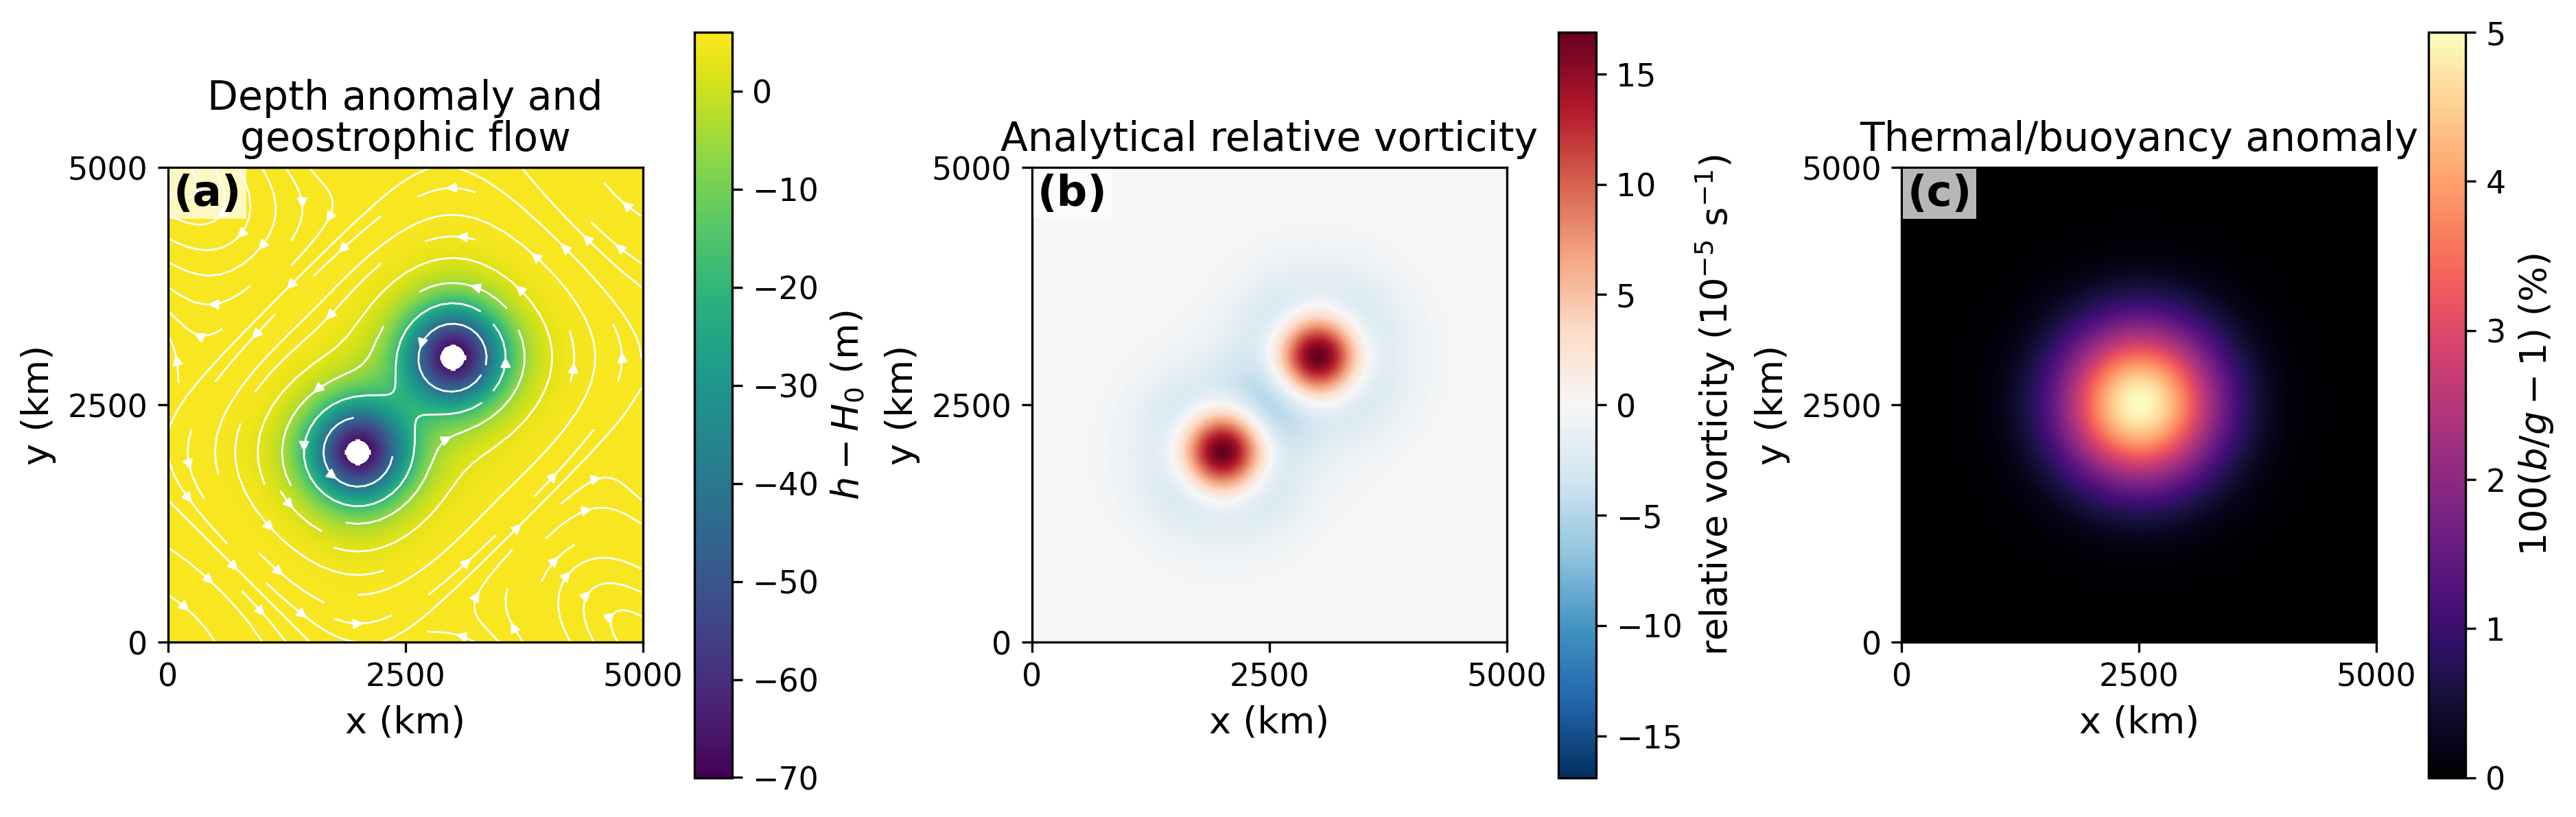
\includegraphics[width=0.98\textwidth]{figure1_doublevortex_initial_state.png}
	\caption{
		Common DoubleVortex initial condition.
		(a) Layer-depth anomaly $h-H_0$ with the analytically constructed
		geostrophic flow.
		(b) Corresponding analytical relative vorticity.
		(c) Central thermal/buoyancy anomaly $100(b/g-1)$, where $b=S/h$.
	}
	\label{fig:doublevortex_initial}
\end{figure}

\subsection{Test 2A: controlled non-raining case}

Test~2A uses a $16\times16$ horizontal mesh and initializes the vapor field at
saturation,
\begin{equation}
	\zeta=0,
	\qquad
	q_v(\mathbf{x},0)=q_{\mathrm{sat}}(\mathbf{x},0).
\end{equation}
The case provides a relatively inexpensive controlled setting in which
condensation and evaporation are active, while rain production does not become
dynamically important. It therefore provides a useful first test of learned
phase-change physics without the additional complication of an active
rain-production rate.


\subsection{Test 2B: rain-active case}

Test~2B increases the horizontal resolution to $64\times64$ cells and modifies
the initial vapor field to produce a modest supersaturation,
\begin{equation}
	\zeta=-0.06,
\end{equation}
so that
\begin{equation}
	q_v(\mathbf{x},0)
	=
	1.06\,q_{\mathrm{sat}}(\mathbf{x},0).
\end{equation}
All other principal DoubleVortex parameters are retained from Test~2A.
The enhanced initial moisture content drives stronger condensation and
cloud-water production, eventually activating the rain-conversion rate $R$.
Test~2B therefore provides the more complete moist-physics problem, in which
both the net phase-change rate $A=E-C$ and the rain-production rate $R$ are
dynamically relevant. It is therefore the principal case used for the
comparison of Representations A, B, and C.

\subsection{Ground-truth evolution and physical diagnostics}

Having established the common DoubleVortex flow and the distinct moisture
initializations of Tests~2A and 2B, we now examine how these differences affect
the subsequent moist evolution. Test~2A remains a non-raining phase-change
case, whereas Test~2B undergoes rapid condensation, cloud-water accumulation,
and eventual activation of the rain-production process. The temporal evolution
of both regimes is summarized in Fig.~\ref{fig:groundtruth_chronology}, followed
by the spatial development of the rain-active Test~2B case and the evolution of
its underlying vortex structure in Fig.~\ref{fig:test2b_gallery}.

Test~2A remains non-raining throughout
the calculation. Its maximum cloud-water mixing ratio is
$3.12\times10^{-5}~\mathrm{kg\,kg^{-1}}$, approximately $31\%$ of the
precipitation threshold
$q_{\mathrm{precip}}=10^{-4}~\mathrm{kg\,kg^{-1}}$, and therefore
$R=Q_r=0$ throughout. Test~2A nevertheless develops regions of both
condensation and evaporation as the vortex flow reorganizes the moisture
field, making it a useful controlled phase-change case without active
cloud-to-rain conversion.

Test~2B evolves very differently. The imposed $6\%$ supersaturation is
consumed rapidly because the condensation timescale is equal to the numerical
timestep, $\tau_v=\Delta t=100~\mathrm{s}$. The initial moist update therefore
converts a large fraction of the excess vapor directly into cloud water,
producing the nearly instantaneous increase in integrated cloud water visible
in Fig.~\ref{fig:groundtruth_chronology}(a). After this initial condensation
pulse, the vortex flow redistributes the cloud and vapor fields and produces
coexisting regions of condensation and evaporation.

The maximum local cloud water eventually reaches the precipitation threshold.
The rain production rate $R$ first becomes nonzero at
\begin{equation}
	t=5100~\mathrm{s}\approx1.42~\mathrm{h},
\end{equation}
and remains active thereafter (Fig.~\ref{fig:groundtruth_chronology}(b)). 
A sustained-rain interval is certified by
$t=6100~\mathrm{s}$. The largest local cloud-water concentration and local
rain-production rate occur near $t=8900~\mathrm{s}$, whereas the
domain-integrated rain-production rate reaches its maximum later, at
\begin{equation}
	t=12000~\mathrm{s}\approx3.33~\mathrm{h}.
\end{equation}
The distinction between these times emphasizes that the first rain event is a
local threshold crossing, whereas the later maximum in integrated rain
production reflects the spatial growth of the rain-producing region.

\begin{figure}[h!]
	\centering
	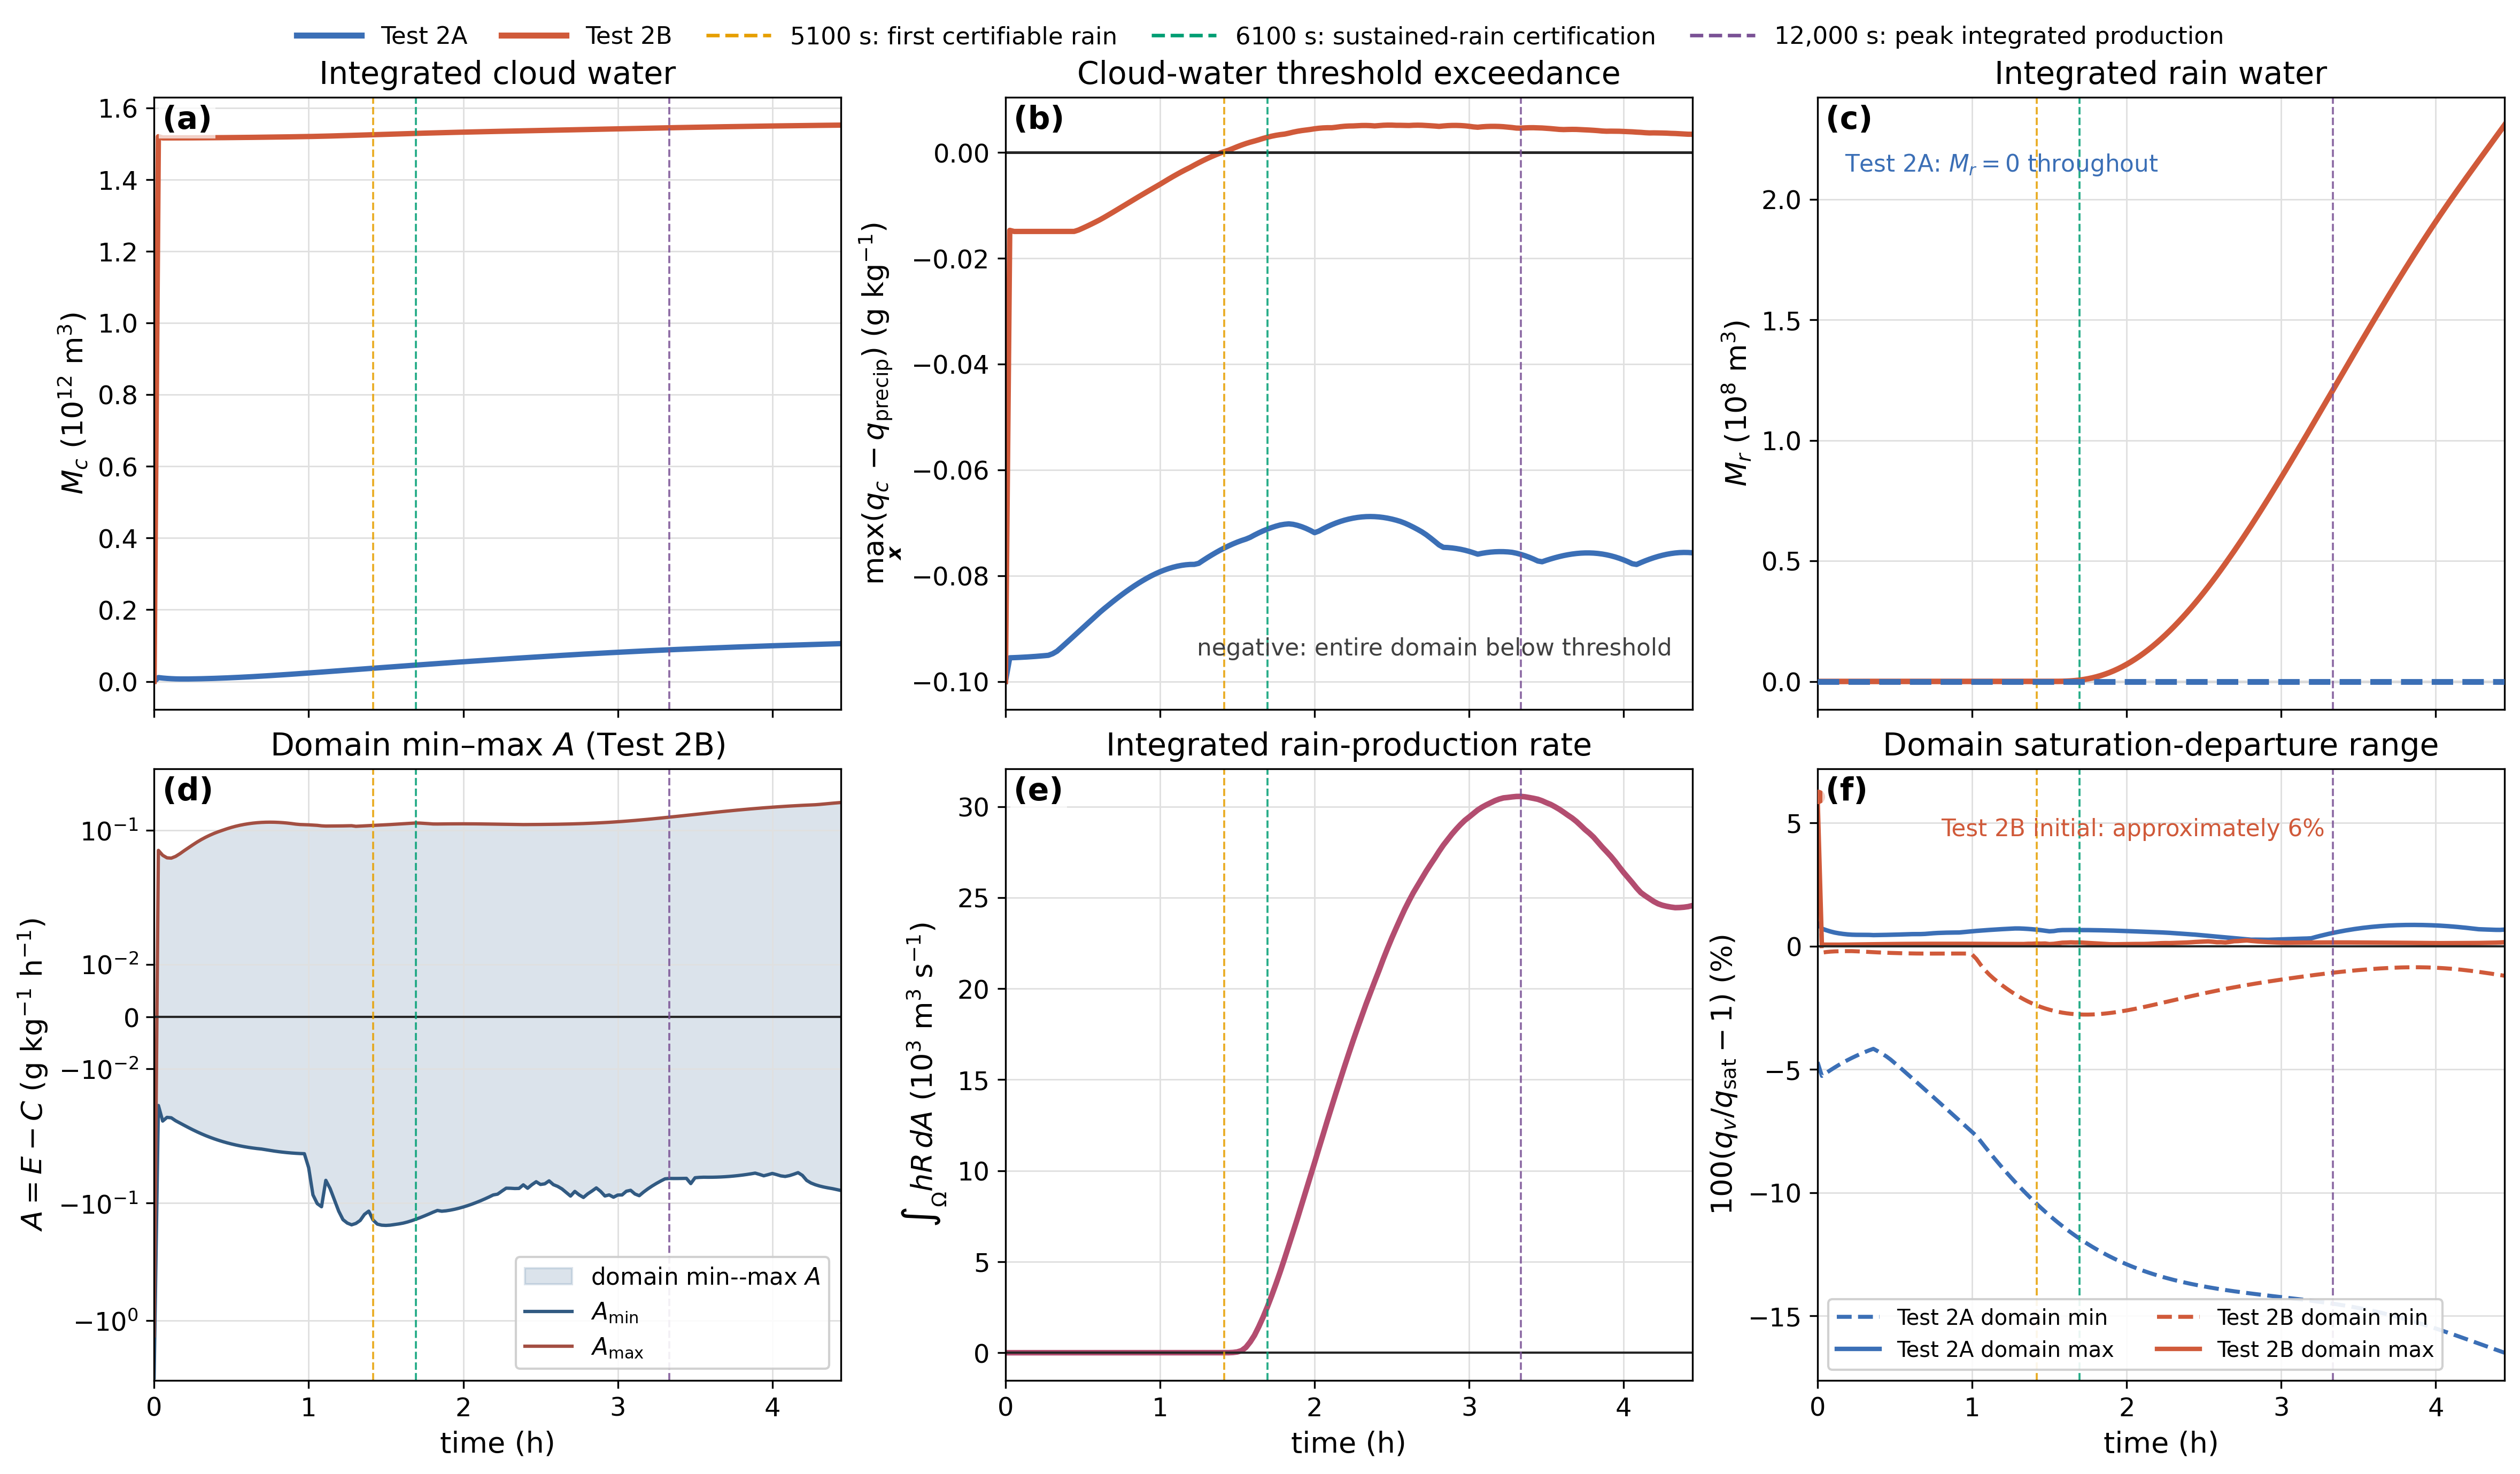
\includegraphics[width=\textwidth]
	{figure2_combined_chronology_regime_comparison.png}
	\caption{
		Ground-truth temporal diagnostics for Test~2A and Test~2B, with emphasis
		on the Test~2B transition to rain.
		(a) Integrated cloud-water reservoir $M_c$.
		(b) Maximum cloud-water threshold exceedance
		$\max_{\mathbf{x}}(q_c-q_{\mathrm{precip}})$; negative values indicate
		that the entire domain remains below the rain threshold.
		(c) Integrated rain-water reservoir $M_r$.
		(d) Domain minimum and maximum of the net phase-change rate
		$A=E-C$ for Test~2B.
		(e) Domain-integrated Test~2B rain-production rate
		$\int_\Omega hR\,dA$.
		(f) Domain minimum and maximum of the post-prefix saturation departure
		$100(q_v/q_{\mathrm{sat}}-1)$ for both cases.
		Vertical dashed lines mark first certifiable rain at $5100~\mathrm{s}$,
		sustained-rain certification at $6100~\mathrm{s}$, and peak integrated
		rain production at $12000~\mathrm{s}$.
		Test~2A and Test~2B differ in both initial vapor loading and spatial
		resolution, so their comparison characterizes distinct moist-physics
		regimes rather than constituting a grid-convergence study.
	}
	\label{fig:groundtruth_chronology}
\end{figure}

The corresponding spatial evolution of Test~2B is shown in
Fig.~\ref{fig:test2b_gallery}. Prior to rain onset, cloud water is
concentrated around the two vortex regions while $R$ remains zero. Once the
cloud-water threshold is crossed, rain production first appears in narrow
localized arcs. These regions are then stretched and wrapped by the vortex
flow into extended curved bands. By the mature-rain state at
$t=12000~\mathrm{s}$, substantial rain production occurs along two broad
spiral-like structures surrounding the vortex cores, while accumulated rain
water occupies a larger region downstream of the actively raining bands. The
final state retains this wrapped two-lobed structure even though the strongest
local rain-production rate has already decreased from its earlier maximum. 
This persistence is expected because the present moist-physics model contains
no rain-removal process such as fallout or rain re-evaporation; $Q_r$ is
therefore transported within the periodic domain once produced.

\begin{figure}[h!]
	\centering
	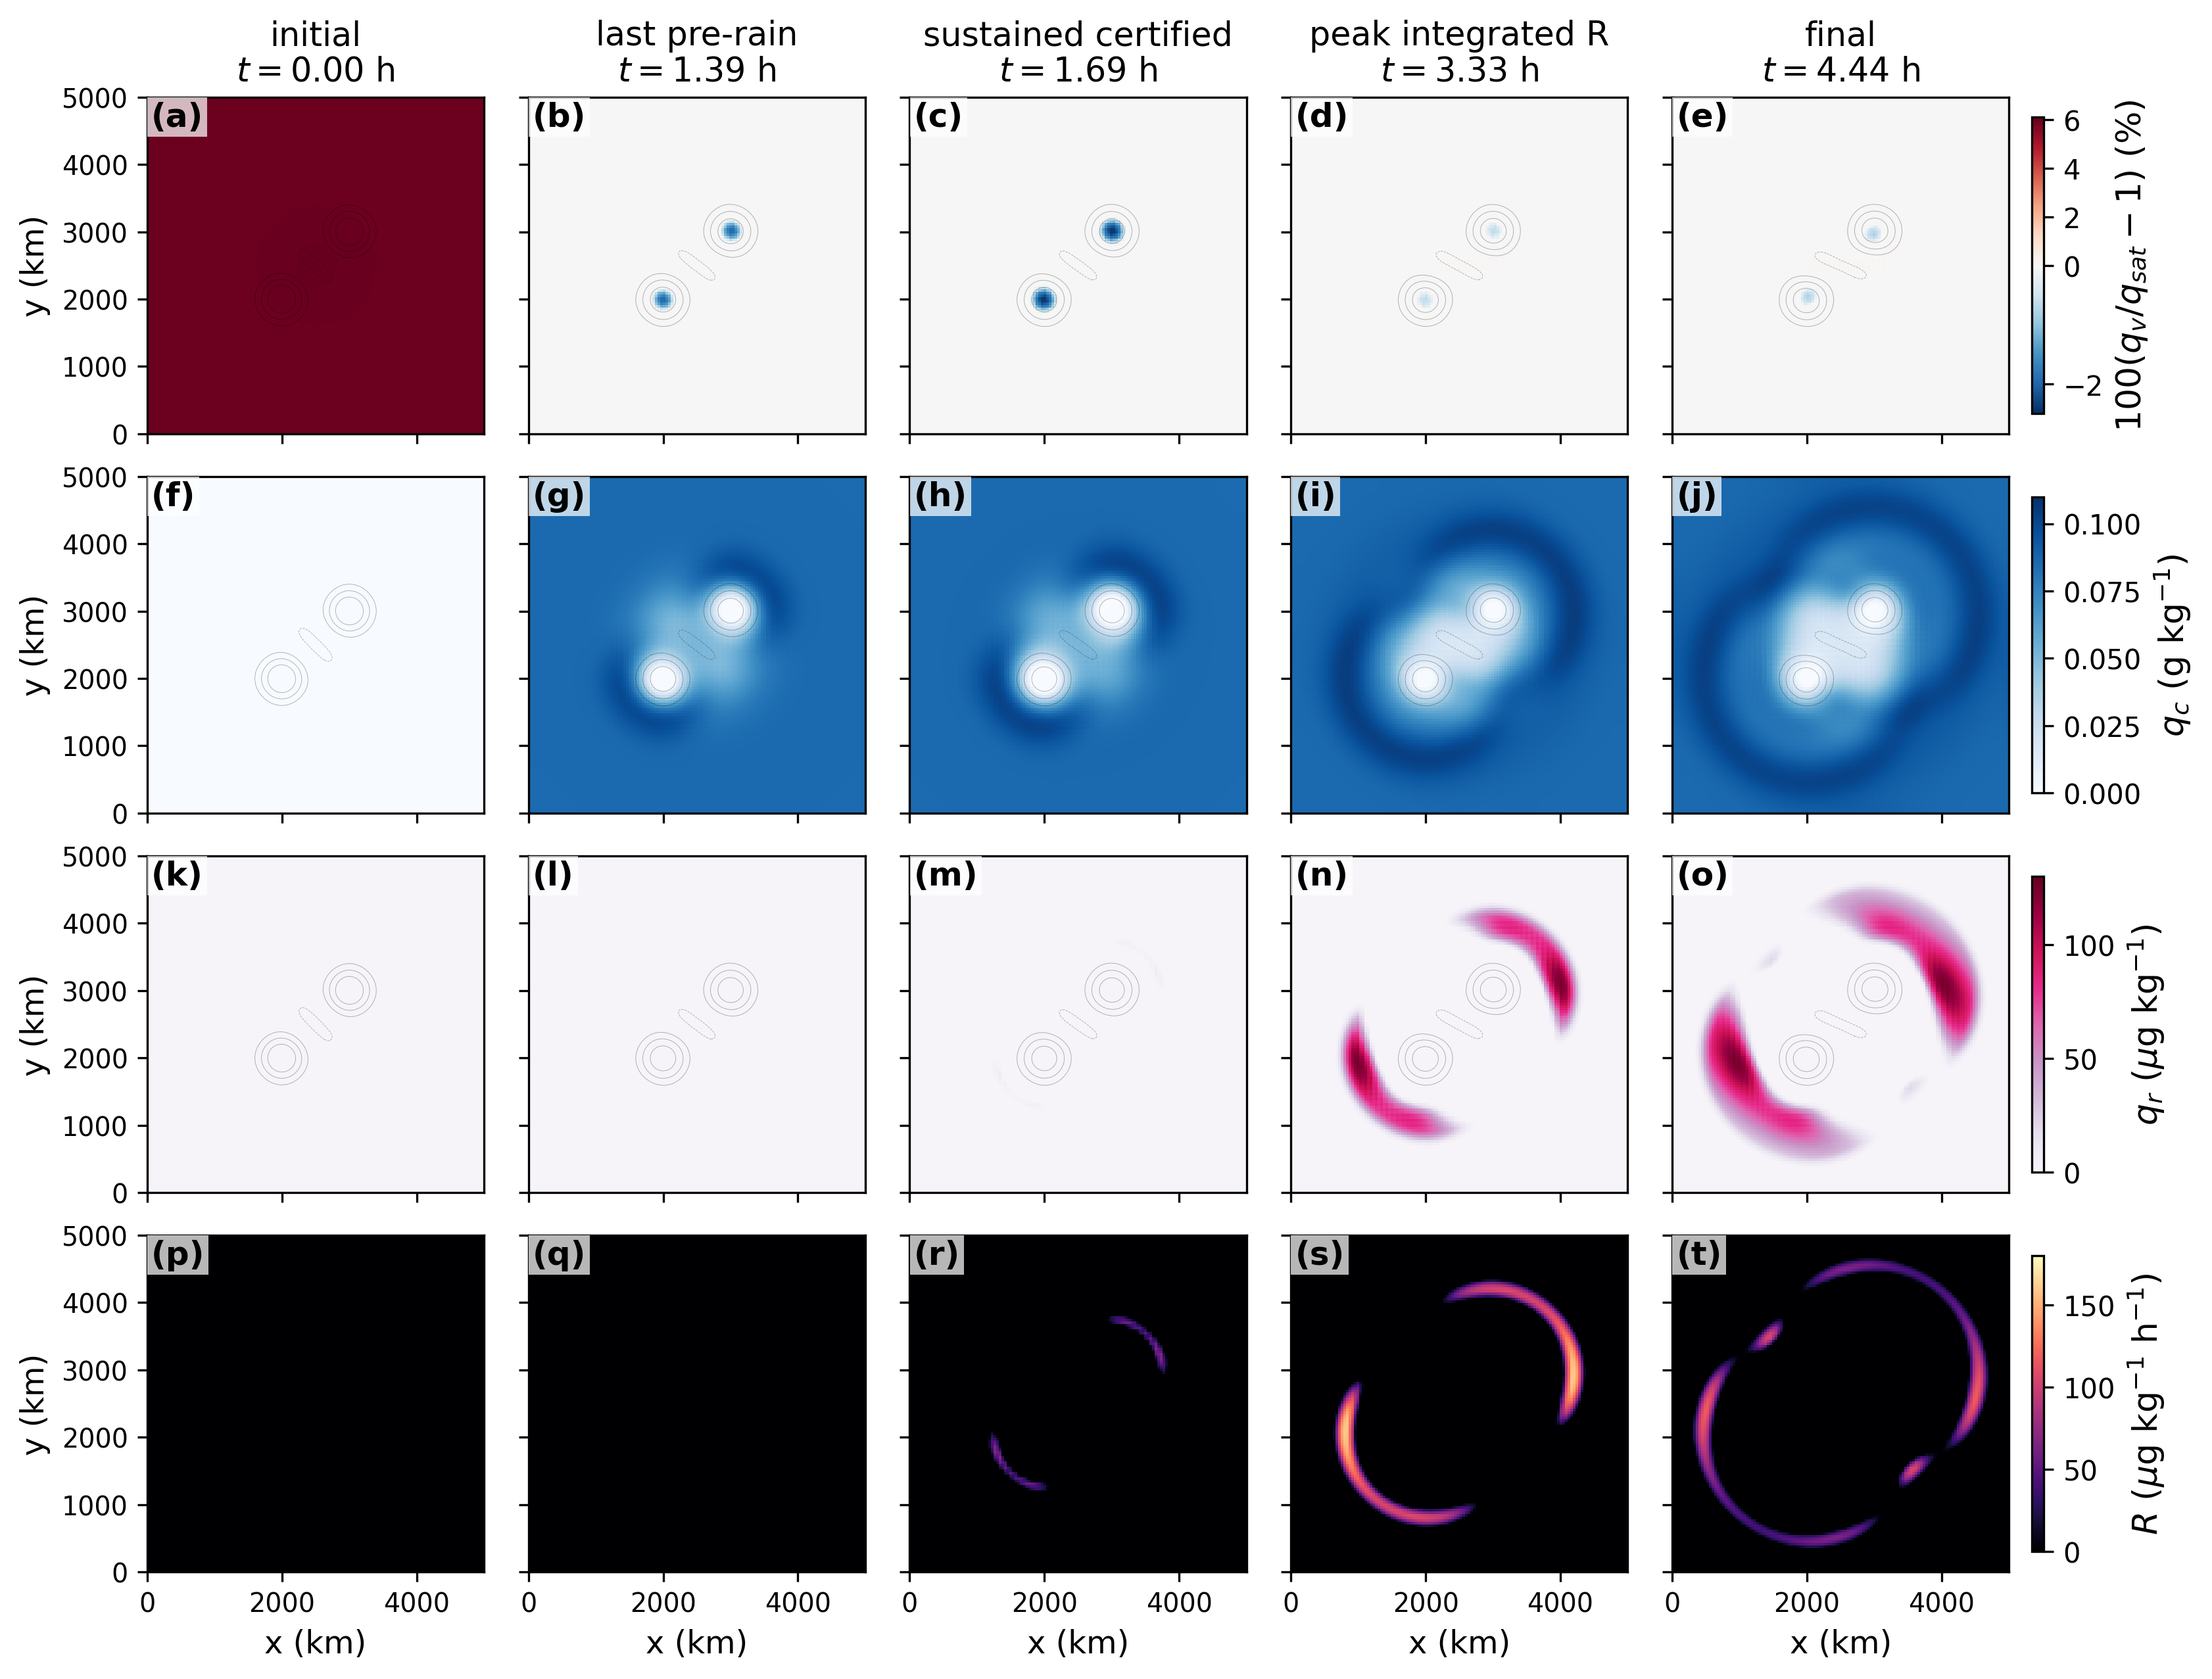
\includegraphics[width=\textwidth]{figure3_test2b_event_gallery.png}
	\caption{
		Spatial evolution of the Test~2B ground-truth solution at five
		physically selected times: the initial state, the last pre-rain state,
		the sustained-rain state, the state of peak integrated rain production,
		and the final state.
		Rows show the saturation departure $100(q_v/q_{\mathrm{sat}}-1)$,
		specific cloud water $q_c$, specific rain water $q_r$, and the
		rain-production rate $R$, respectively.
		Gray relative-vorticity contours indicate the locations of the two
		vortex cores.
		Rain production first develops in narrow arcs near regions of enhanced
		cloud water and is subsequently stretched into extended curved bands by
		the vortex flow.
	}
	\label{fig:test2b_gallery}
\end{figure}

The strong deformation visible in Fig.~\ref{fig:test2b_gallery} and in the
truth-evolution movie occurs with remarkably little translation of the
underlying vortex pair. Figure~\ref{fig:test2b_vortex_motion} tracks the two
positive-vorticity cores using continuously followed local
vorticity-weighted centroids. Over the full $16000~\mathrm{s}$ simulation,
the maximum displacement of either core is only $18.0~\mathrm{km}$, or
$0.36\%$ of the domain size and $4.8\%$ of the characteristic vortex width
$\sigma=375~\mathrm{km}$. The pair separation changes by approximately
$27~\mathrm{km}$ and its orientation by less than $1^\circ$, while the
pair midpoint remains fixed to numerical precision. Thus the dominant moist
evolution is material deformation and wrapping around an approximately
stationary vortex skeleton rather than bulk translation of the vortices.

\begin{figure}[h!]
	\centering
	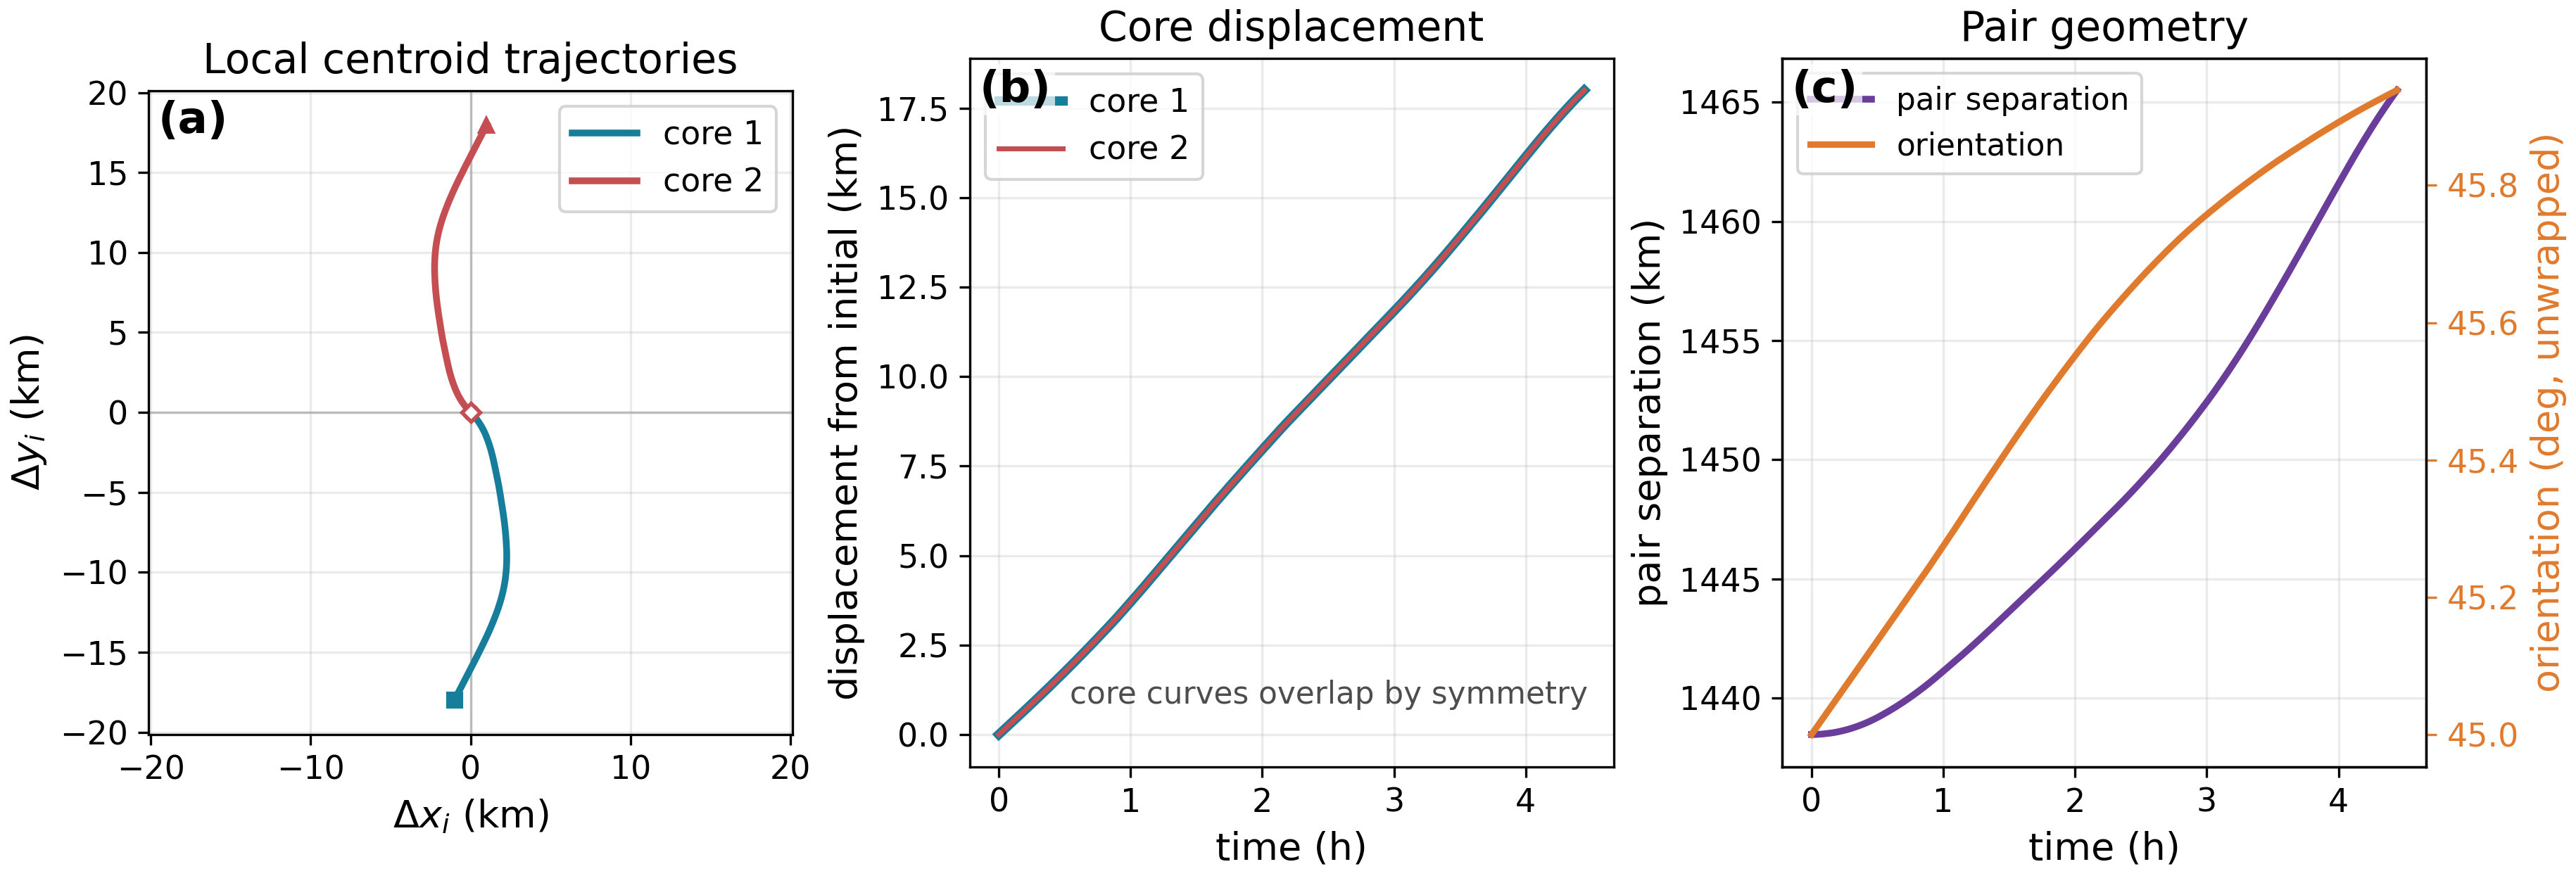
\includegraphics[width=0.98\textwidth]
	{figure5_test2b_vortex_core_motion.png}
	\caption{
		Motion of the two positive-vorticity cores during the Test~2B
		ground-truth simulation, measured using continuously tracked local
		vorticity-weighted centroids.
		(a) Core trajectories relative to their respective initial positions,
		shown as $(\Delta x_i,\Delta y_i)$.
		(b) Displacement magnitude of each core from its initial position; the
		two curves nearly overlap because of the symmetry of the vortex pair.
		(c) Separation and unwrapped orientation of the vortex pair.
		The maximum core displacement is only about $18~\mathrm{km}$, showing
		that the pronounced evolution of the cloud and rain fields is dominated
		by deformation and advection around a nearly stationary vortex pair.
	}
	\label{fig:test2b_vortex_motion}
\end{figure}


\section{Machine-Learning Results}\label{sec:MLResults}
\subsection{Training and evaluation data}

The machine-learning results presented below use the higher-resolution
$64\times64$ rain-active DoubleVortex trajectory described in
Sec.~\ref{sec:PhysicalSims}. The trajectory contains 161 stored states,
indexed from $0$ to $160$. States $0$--$80$ are used for training, while
states $81$--$160$ are reserved for evaluation after training. The latter
therefore assess temporal generalization beyond the portion of the trajectory
used for fitting.

Each stored state contributes $65{,}536$ local spatial samples
($64^2$ cells $\times\,4^2$ Gauss--Lobatto--Legendre quadrature points per
cell), giving $5{,}308{,}416$ ($65{,}536\times 81$) training samples across states $0$--$80$ and
$5{,}242{,}880$ evaluation samples across states $81$--$160$. Not all of them are active rain samples.

\subsection{Optimization of the training objectives}

Figure~\ref{fig:ml_optimization} shows the reduction of the M1-Y, H1,
H2, and H5 training objectives for the three learned-physics
representations. Because network parameters were retained only at selected
iterations, the curves show the objective at those saved points rather than
at every optimization iteration.

For all three representations, M1-Y reduces the direct physical-law
objective by several orders of magnitude over the $10{,}000$
iterations. In this initial exploratory investigation we set a maximum of $10{,}000$ for $M1-Y$ unless the objective falls below $10^{-8}$. Thus the we have not fully optimized the Network parmeters yet.

The H1/M2-Y objective also decreases throughout its $5{,}000$-iteration
optimization for all three representations. This is also stopped by a cutoff and hence H1 network could also be further optimized. H1 begins from an already trained
direct-regression model, and its one-step objective is therefore already
relatively small at the start of this optimization stage.

H2 is initialized from H1, and H5 is subsequently initialized from H2.
Each recursive stage is limited to 20 iterations. Only their initial and
final objective values are shown. These short continuation stages produce
little change for Representations A and B, whereas Representation C shows a
more noticeable reduction (it starts from a higher objective value than A and B). The H2 and H5 results should therefore be
interpreted together with their short optimization budgets and sequential
initialization.

The numerical values of M1-Y, H1, H2, and H5 are not directly comparable
because the objectives measure different quantities. Figure~\ref{fig:ml_optimization}
is therefore used only to assess the reduction achieved for each objective
during its own optimization.


\begin{figure}[h!]
	\centering
	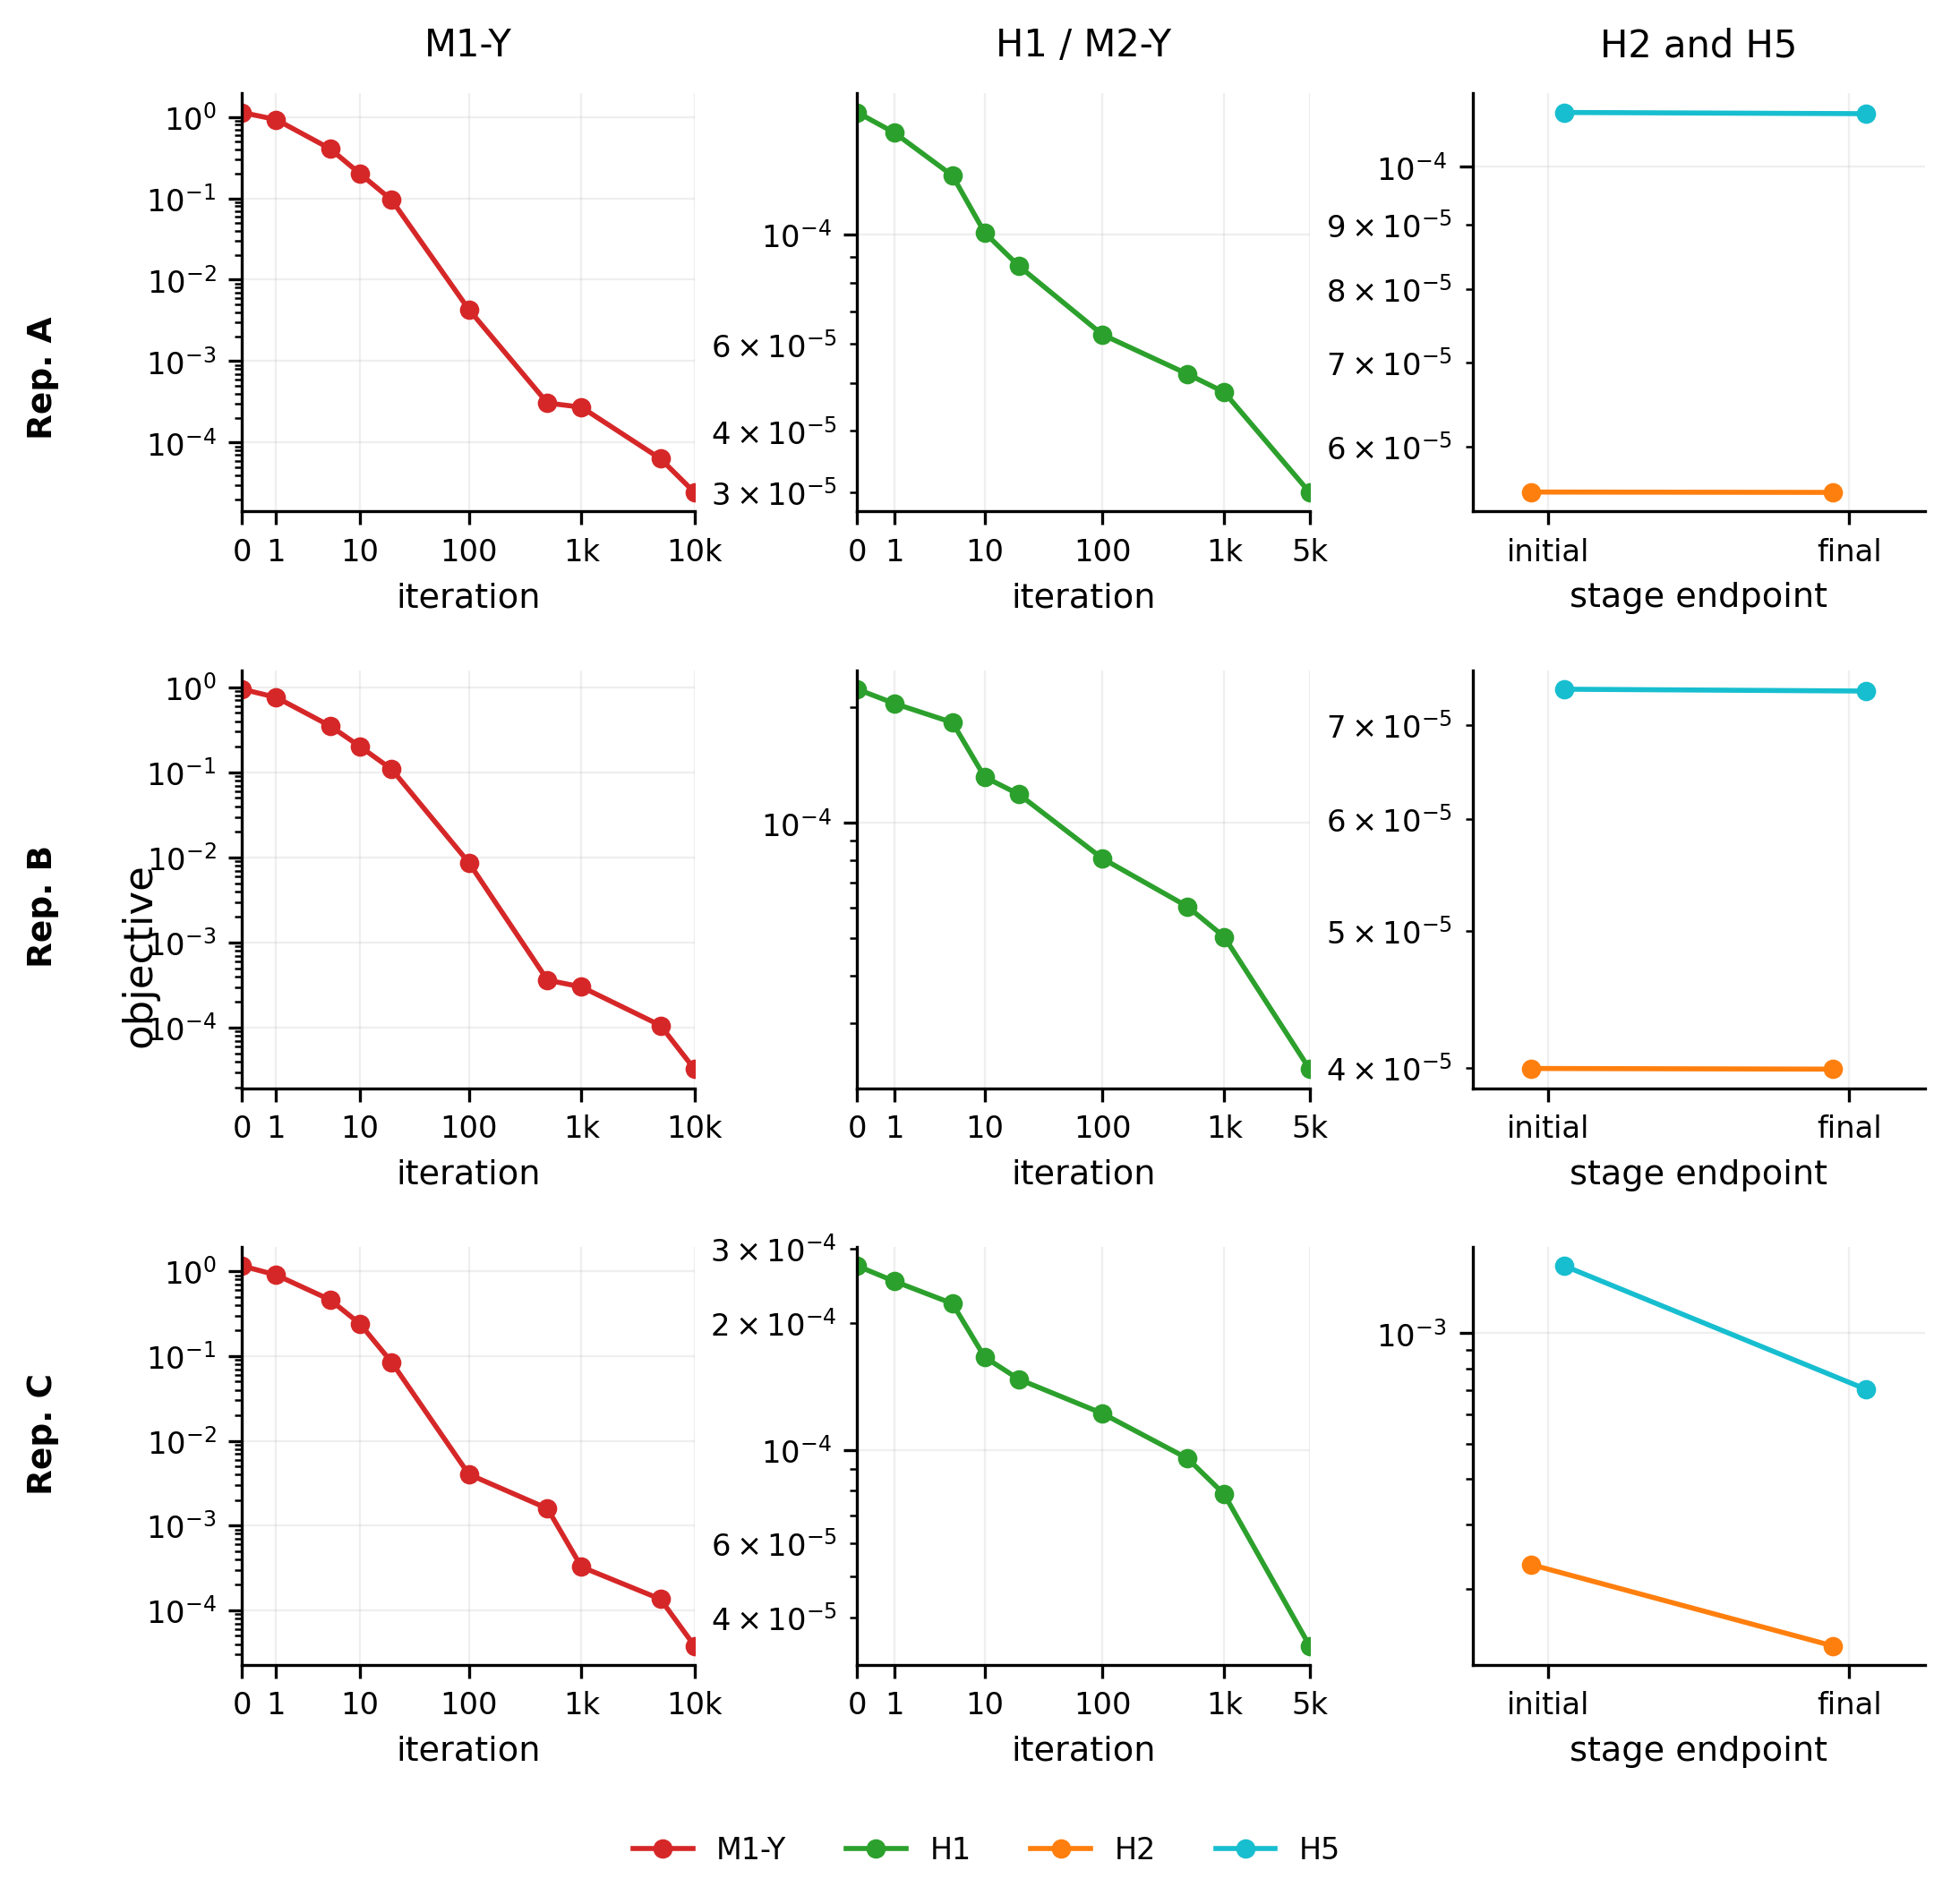
\includegraphics[width=\textwidth]
	{ML1_main_optimization.png}
	\caption{
		Optimization of the Test~2B training objectives for
		Representations A--C.
		The left column shows M1-Y, which fits the local analytical moist
		physics at the pre-moist state $Y^\star$.
		The middle column shows the one-step H1/M2-Y objective.
		The right column shows the initial and final values of the recursive
		H2 and H5 objectives.
		Markers in the M1-Y and H1 panels indicate iterations at which the
		network parameters were saved.
		H2 and H5 were each limited to 20 iterations, and only their initial
		and final objective values are shown.
		Because the objectives and their normalizations differ, numerical
		values should not be compared between different objective types or
		representations.
	}
	\label{fig:ml_optimization}
\end{figure}

\subsection{Training and evaluation errors}

We next examine whether the quantities minimized during training remain
accurate over the later portion of the DoubleVortex trajectory.
Figure~\ref{fig:ml_training_evaluation} compares each fitted objective over
the training states $0$--$80$ (solid curves) and the evaluation states $81$--$160$ (dashed curves). 

For M1-Y, the network is trained directly against the local analytical moist
physics at the pre-moist states $Y^\star$. The training objective decreases by
several orders of magnitude for all three representations. The corresponding
evaluation error remains substantially larger, however, indicating that the
accuracy obtained over the fitted portion of the trajectory does not extend
uniformly to its later evolution. The M1-Y training objective is still
decreasing at the end of the prescribed $10{,}000$ iterations, so additional
optimization could further improve the fit to the training data. Whether it
would also reduce the evaluation error is not established by the present
calculations.

A similar training--evaluation separation is observed for H1/M2-Y, but here
the quantity being minimized is the one-step state error rather than the local
moist-physics error. The state error becomes small over the training interval,
while the same one-step prediction problem remains considerably more difficult
over the evaluation interval.

The distinction between the two objectives is worth noting. In M1-Y the loss
acts directly on the quantities predicted by the network: $A$, $(A,R)$, or
the moist-source vector. In H1/M2-Y, the network outputs first pass through
the discrete source-to-state mapping before the loss is evaluated on the
resulting state increment. The M1-Y regression problem is therefore more
directly tied to the network outputs, whereas H1 asks the optimizer to infer
the local physics through its effect on the numerical state. The results in
Fig.~\ref{fig:ml_training_evaluation} suggest that the simpler direct
regression is easier to fit and generalize in the present configuration.
This conclusion is specific to the network size, training data, and
optimization budgets used here; greater model capacity or broader training
data could alter the comparison.

\begin{figure}[h!]
	\centering
	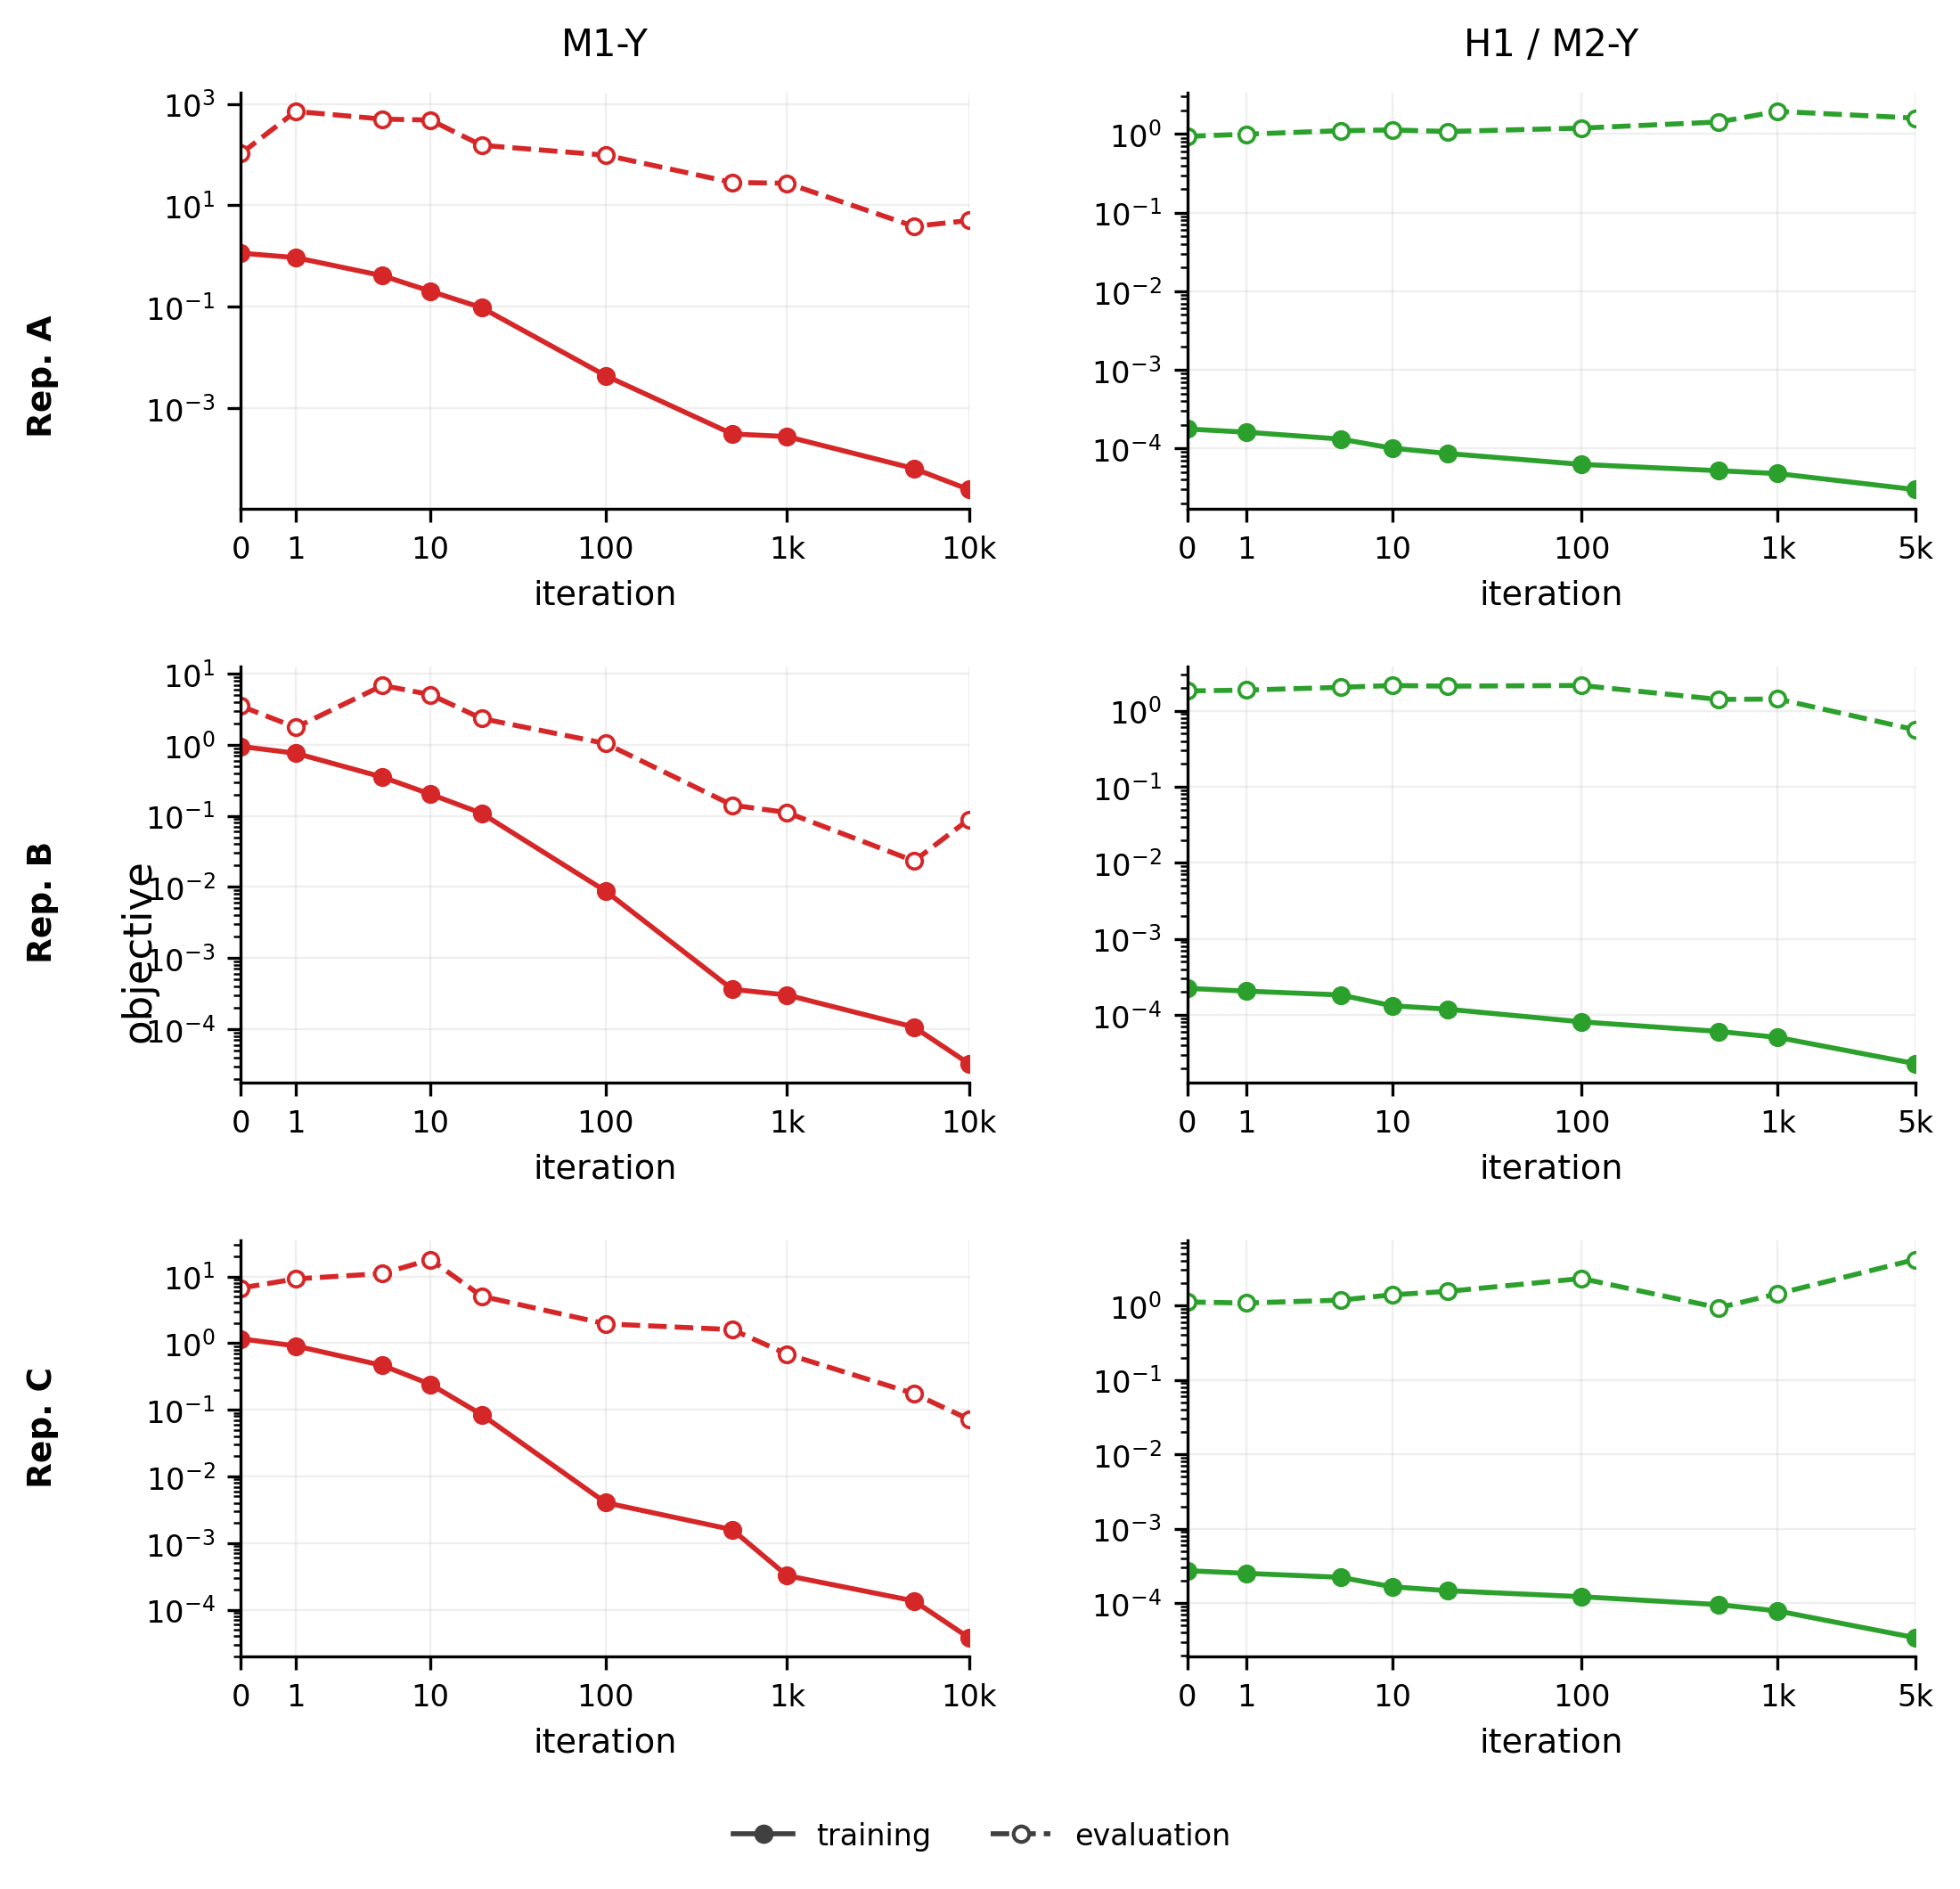
\includegraphics[width=\textwidth]
	{ML2_main_training_evaluation.png}
	\caption{
	Training and evaluation errors for M1-Y and H1/M2-Y in
	Representations A--C.
	The left column shows the M1-Y direct physical-law objective evaluated
	at the pre-moist states $Y^\star$, and the right column shows the
	H1/M2-Y one-step state objective.
	Solid curves show the objective over the training portion of the
	trajectory, while dashed curves with open symbols show the same
	objective over the later evaluation portion.
	The evaluation data do not influence the optimization.
	Objective normalizations differ among representations and between
	M1-Y and H1/M2-Y, so numerical values should be interpreted within
	each panel rather than compared directly across panels.
}

	\label{fig:ml_training_evaluation}
\end{figure}

The training--evaluation gap is substantial for both objectives and for all
three representations. Thus a small training error alone is not sufficient to
establish that the learned parameterization remains accurate as the system
moves into later portions of the trajectory. We next compare the final
networks using a common physical diagnostic: their ability to reproduce the
local moist physics at the pre-moist state $Y^\star$.
	
\subsection{Accuracy of the learned moist physics}

The preceding comparison measures each training method using the objective for
which it was optimized. We now compare the final networks using a common
physical measure: how accurately they reproduce the moist-physics forcing, or
the part of the forcing replaced by the network, when evaluated at the
truth-derived pre-moist state $Y^\star$. Figure~\ref{fig:ml_callsite_accuracy}
shows this comparison for the final M1-Y, H1, H2, and H5 networks, separately
over the training (filled symbols) and evaluation (open symbols) portions of
the trajectory.


For Representation A, all four models reproduce the phase-change rate $A$
accurately over the training interval, with relative RMS errors below
$10^{-2}$. The errors are substantially larger over the evaluation interval,
where none of the models retains the same level of accuracy. H1, H2, and H5
nevertheless give smaller evaluation errors in $A$ than M1-Y, with relative
RMS errors of about $1.3$ compared with approximately $2.24$ for M1-Y.
Thus, although H1 is not trained by directly minimizing the local error in
$A$, the resulting H1, H2, and H5 networks give smaller later-time errors in
this quantity than M1-Y. This comparison also illustrates why the objective
values in Fig.~\ref{fig:ml_training_evaluation} should not be used to rank
M1-Y and H1 directly: they measure different quantities, whereas the present
figure evaluates both networks using the same physical error in $A$.

A similar reduction in the evaluation error of $A$ is found for
Representation B. \textbf{The behavior of the learned rain rate $R$, however,
	is very different.} M1-Y reproduces the analytical rain law with relative RMS
errors of only a few percent on both the training and evaluation intervals.
In contrast, the H1, H2, and H5 models have errors of approximately $0.5$ over
the rain-active samples. Thus the models obtained from the state-based
objectives give smaller later-time errors in $A$ but substantially poorer
recovery of the thresholded rain process.

Representation C shows an even stronger distinction. M1-Y closely reproduces
the four-component moist source over the training interval and retains a
source-vector relative RMS error of approximately $0.27$ over the evaluation
interval. The H1, H2, and H5 models have considerably larger source-vector
errors, approximately $0.9$ on the evaluation interval. Thus, although these
models were trained to improve the evolution of the numerical state, they
recover the underlying four-component moist source considerably less
accurately than the direct physical-law regression.

These results show that reducing a state-based training objective does not
necessarily improve the fidelity of every local physical process represented
by the network. This distinction is particularly important for
Representations B and C, where the network is given additional freedom to
represent the rain process or the complete moist-source vector. We next examine
whether these differences in local physical accuracy lead to corresponding
differences when the learned parameterizations are actually deployed in the
DIMSWE simulation.

\begin{figure}[h!]
	\centering
	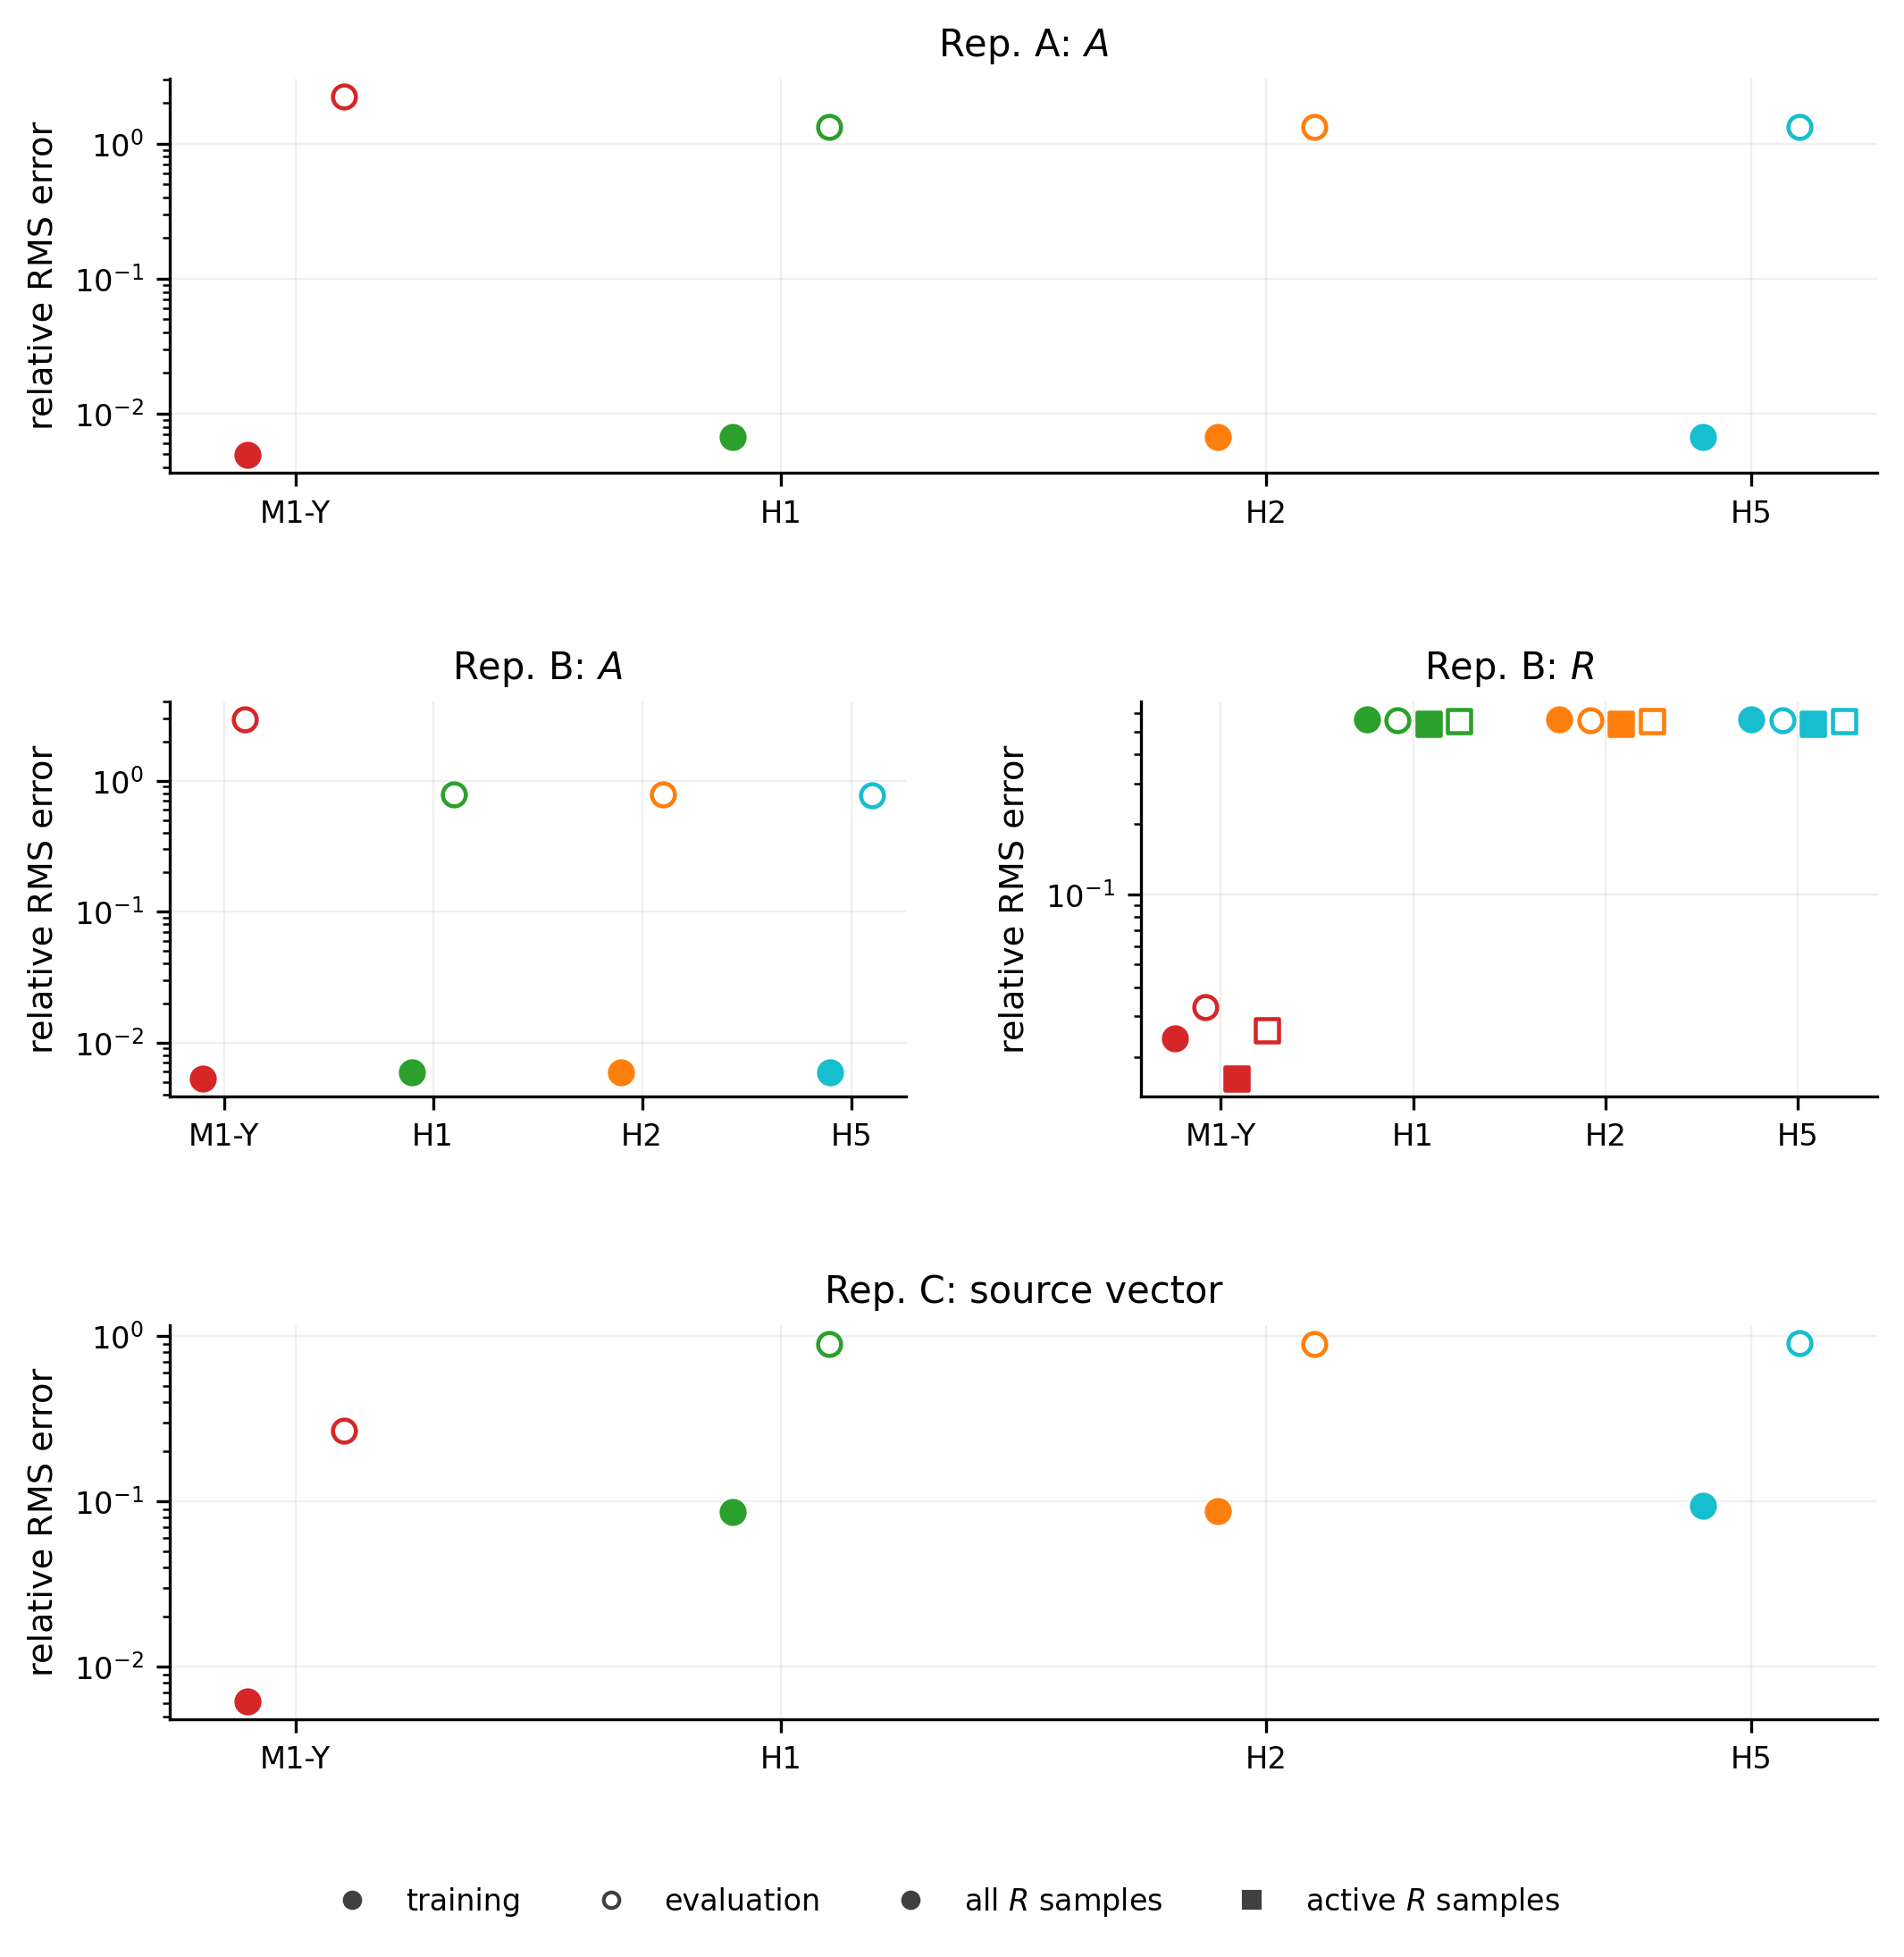
\includegraphics[width=\textwidth]
	{ML3_main_callsite_physical_accuracy.png}
	\caption{
		Accuracy of the final learned moist-physics models evaluated at the
		pre-moist truth states $Y^\star$.
		Filled symbols correspond to training states $0$--$80$ and open symbols
		to evaluation states $81$--$160$.
		For Representation A, the error is measured in the phase-change rate
		$A$.
		For Representation B, separate panels show errors in $A$ and $R$; the
		$R$ panel distinguishes errors over all samples and over samples for
		which the analytical rain rate is active.
		For Representation C, the plotted quantity is the normalized
		source-vector relative RMS error. $Y^\star$ is the truth-derived pre-moist state corresponding to the
		moist-physics call site in the split timestep.
	}
	\label{fig:ml_callsite_accuracy}
\end{figure}

\subsection{Physical behavior after deployment}

We next examine the learned parameterizations after they are embedded in the
DIMSWE timestep and allowed to evolve the model state. Figure~
\ref{fig:ml_deployed_diagnostics} summarizes several diagnostics of the final
deployed solutions for M1-Y, H1, H2, and H5.

The three representations behave quite differently with respect to
conservation. Representations A and B preserve the total-water and
thermodynamic source identities by construction, and their total-water drift
remains at approximately roundoff level for all four training objectives.
Representation C does not impose these identities, and its total-water drift
increases along the sequence M1-Y $\rightarrow$ H1 $\rightarrow$ H2
$\rightarrow$ H5.

The final state errors show a similar pattern. Representations A and B remain
accurate for all four training objectives, with relative errors of order
$10^{-5}$ or smaller. Representation C is also accurate for M1-Y, but its
final state error increases markedly for H1, H2, and H5, reaching order
$10^{-3}$ for H5. \textbf{Thus, for the unconstrained source representation, increasing the
complexity of the training objective (which requires online training) does not improve long-time deployment.}

None of the representations explicitly enforces non-negativity of the
discrete moisture fields. Negative values occur in the discrete moisture
variables $Q_v$, $Q_c$, and $Q_r$ for all three representations, with
substantially larger violations for Representation C after H1, H2, and H5
training. The rain and cloud mass
diagnostics show a similar distinction. Representations A and B retain
comparatively small errors in the final water partition, whereas
Representation C develops substantially larger cloud- and rain-mass errors,
particularly for the state-based and recursive objectives.

Rain onset provides an additional diagnostic of the learned rain process.
Representation A retains the analytical rain law and reproduces
the truth onset time. In Representations B and C, the learned rain tendency is
not constrained to reproduce the analytical threshold exactly, and nonzero
rain production appears before the truth onset. Because an arbitrarily small
positive learned tendency can trigger this timing diagnostic, the onset error
is best interpreted together with the rain-rate and water-partition errors
rather than as a measure of rain accuracy by itself.

\begin{figure}[h!]
	\centering
	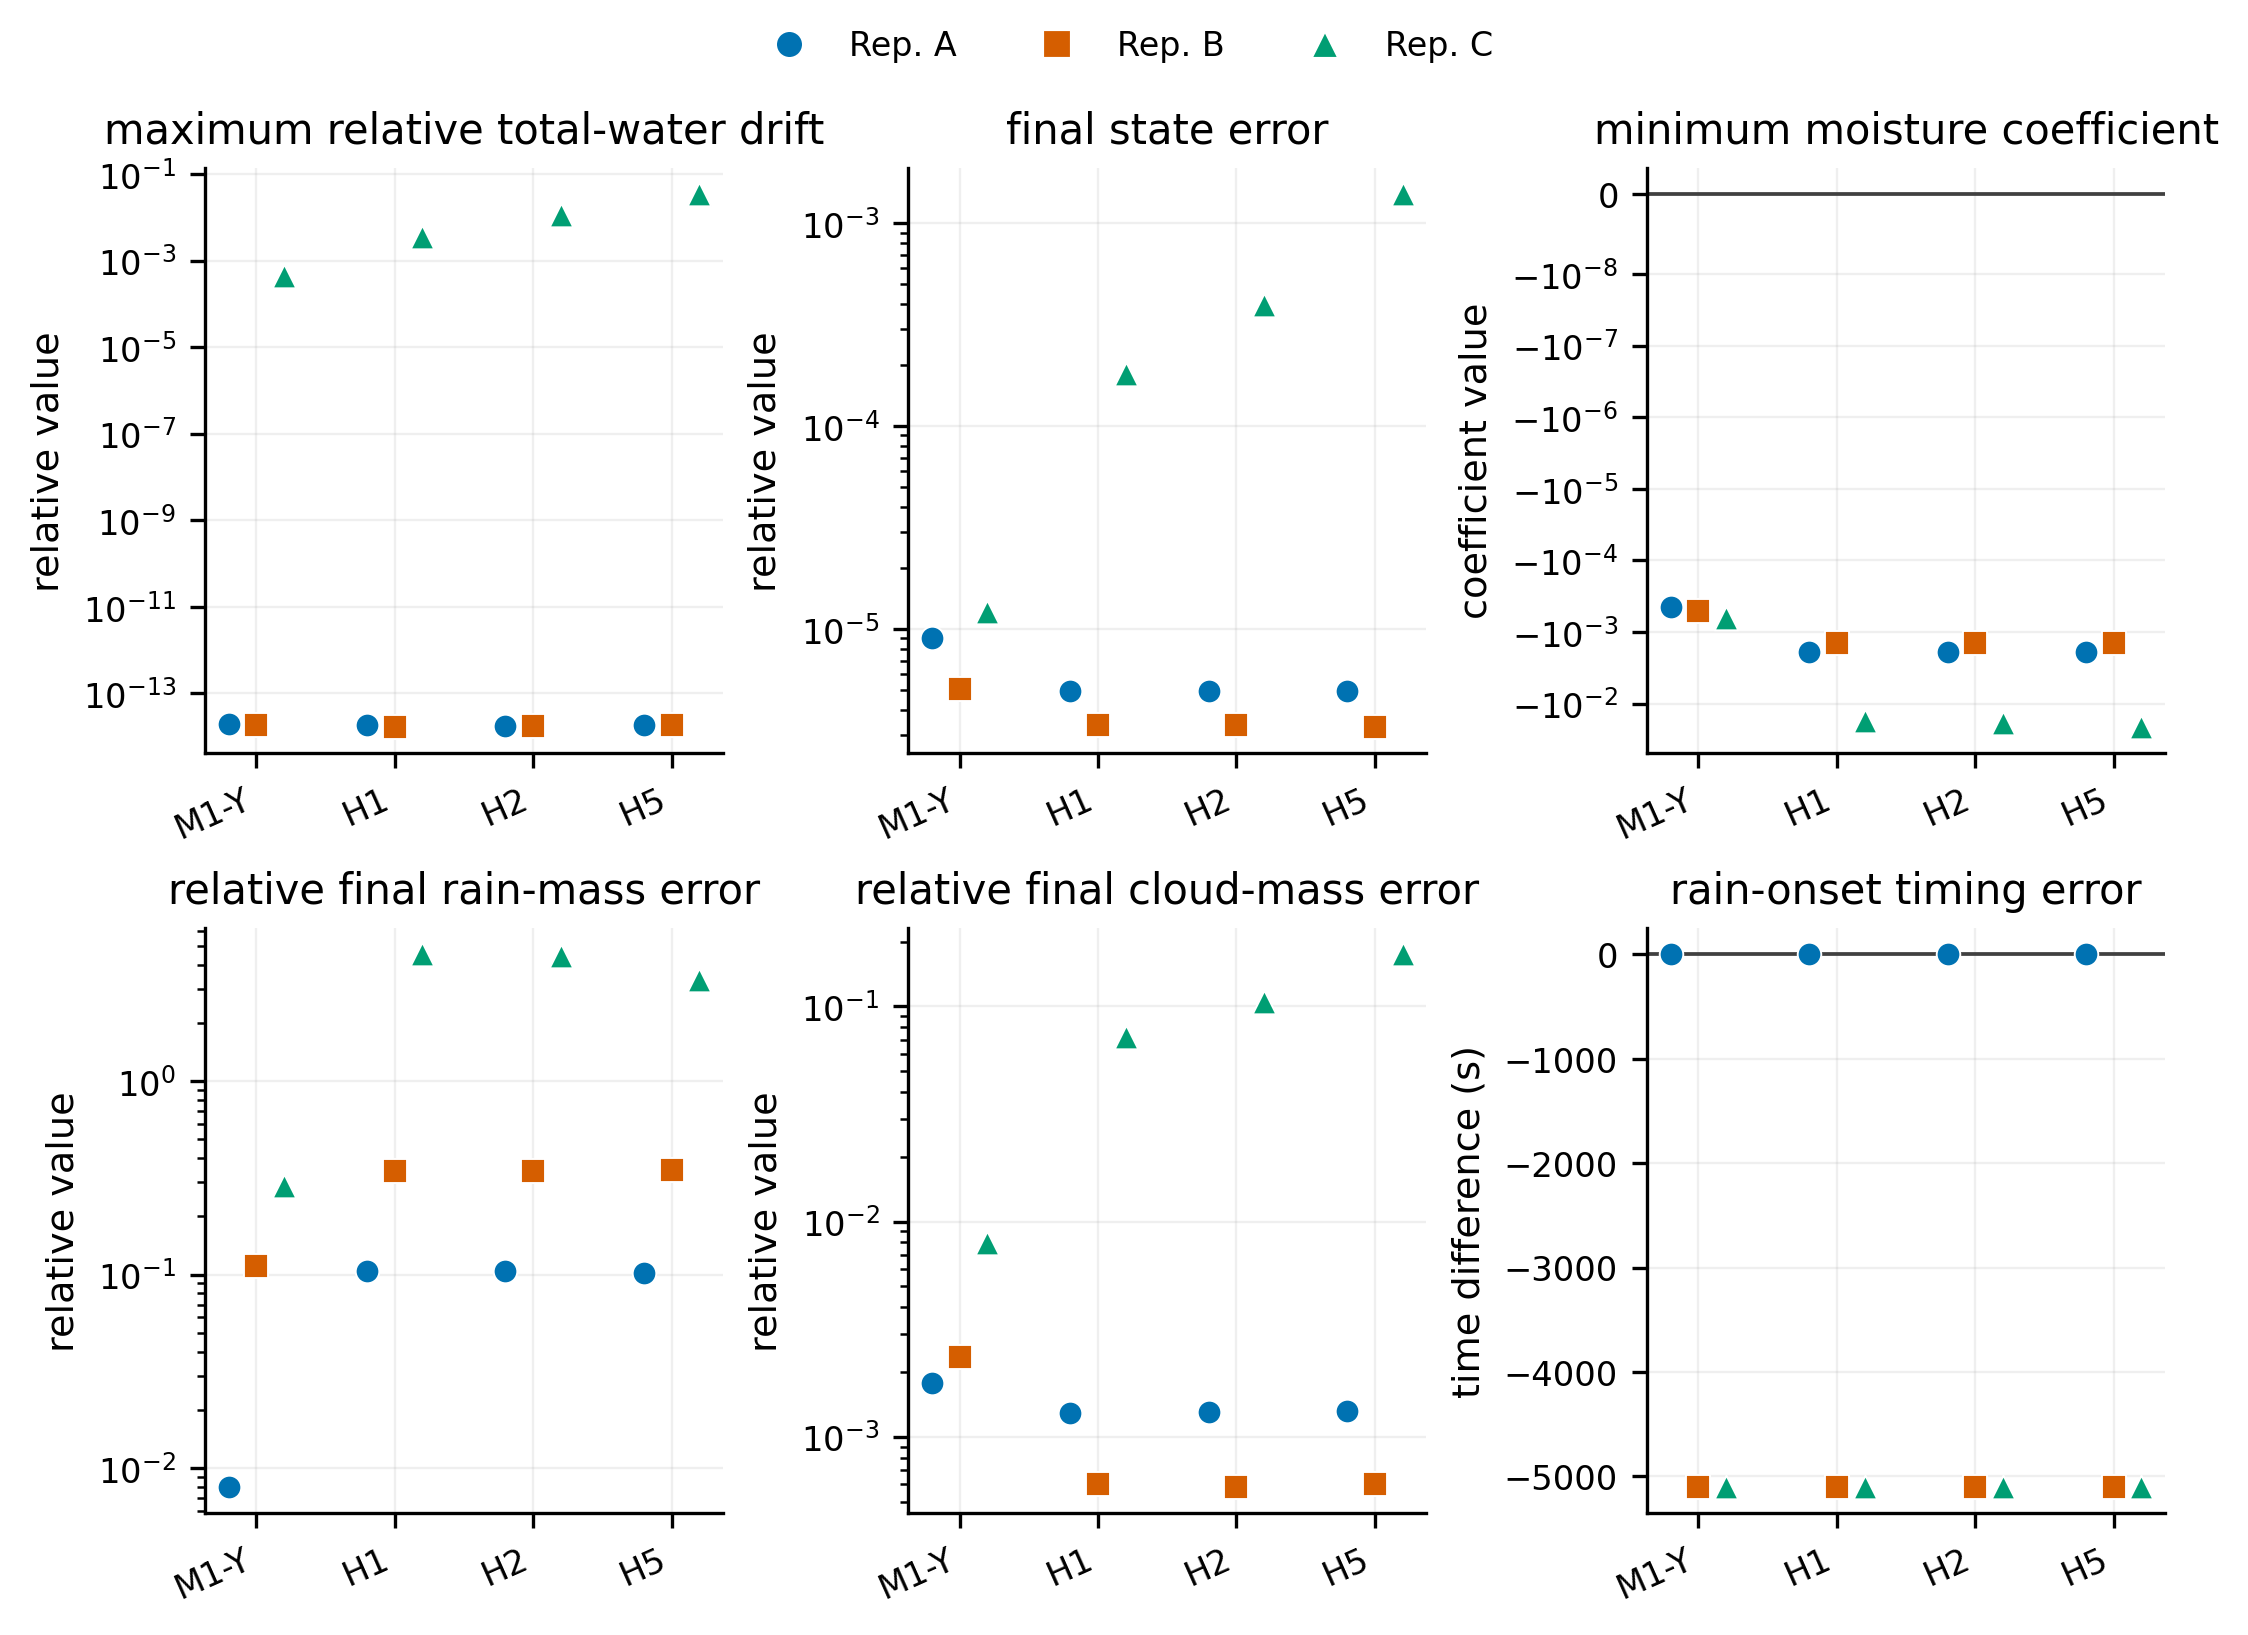
\includegraphics[width=\textwidth]
	{ML4_main_deployed_physical_diagnostics.png}
	\caption{
		Physical diagnostics of the deployed Test~2B models for
		Representations A--C.
		The panels show the maximum relative total-water drift, final relative
		state error, minimum moisture coefficient, relative errors in the final
		rain- and cloud-water masses, and the difference in rain-onset time
		relative to truth.
		Representations A and B enforce the total-water and thermodynamic source
		identities algebraically, whereas Representation C learns the four
		source components independently; the corresponding conservation errors
		therefore have different interpretations.
		The reported moisture minima are finite-element coefficient minima and
		should not be interpreted as a pointwise positivity guarantee for the
		reconstructed continuous fields.
	}
	\label{fig:ml_deployed_diagnostics}
\end{figure}
	
	\subsection{Global evolution of the deployed models}
	
	The endpoint diagnostics in Fig.~\ref{fig:ml_deployed_diagnostics} summarize
	the final accuracy of the deployed models, but do not show how the differences
	develop during the simulation. Figures~\ref{fig:ml_global_A}--\ref{fig:ml_global_C}
	therefore compare several domain-integrated and flow diagnostics throughout
	the full DoubleVortex trajectory.
	
	For Representation A, all four learned models reproduce the cloud- and
	rain-water evolution closely (Fig.~\ref{fig:ml_global_A}). The total-water
	drift remains at roundoff level, as expected from the prescribed source
	structure. Differences among the training objectives are more apparent in the
	flow diagnostics: M1-Y remains relatively close to the truth in kinetic energy
	and projected relative-vorticity squared, while H1, H2, and H5 develop somewhat
	larger deviations late in the simulation. Nevertheless, the overall state
	errors remain small for all four models. Thus, when only the phase-change rate
	$A$ is learned and the analytical rain law and source structure are retained,
	the deployed solution is comparatively insensitive to the choice among the
	four training objectives.
	
	\begin{figure}[h!]
		\centering
		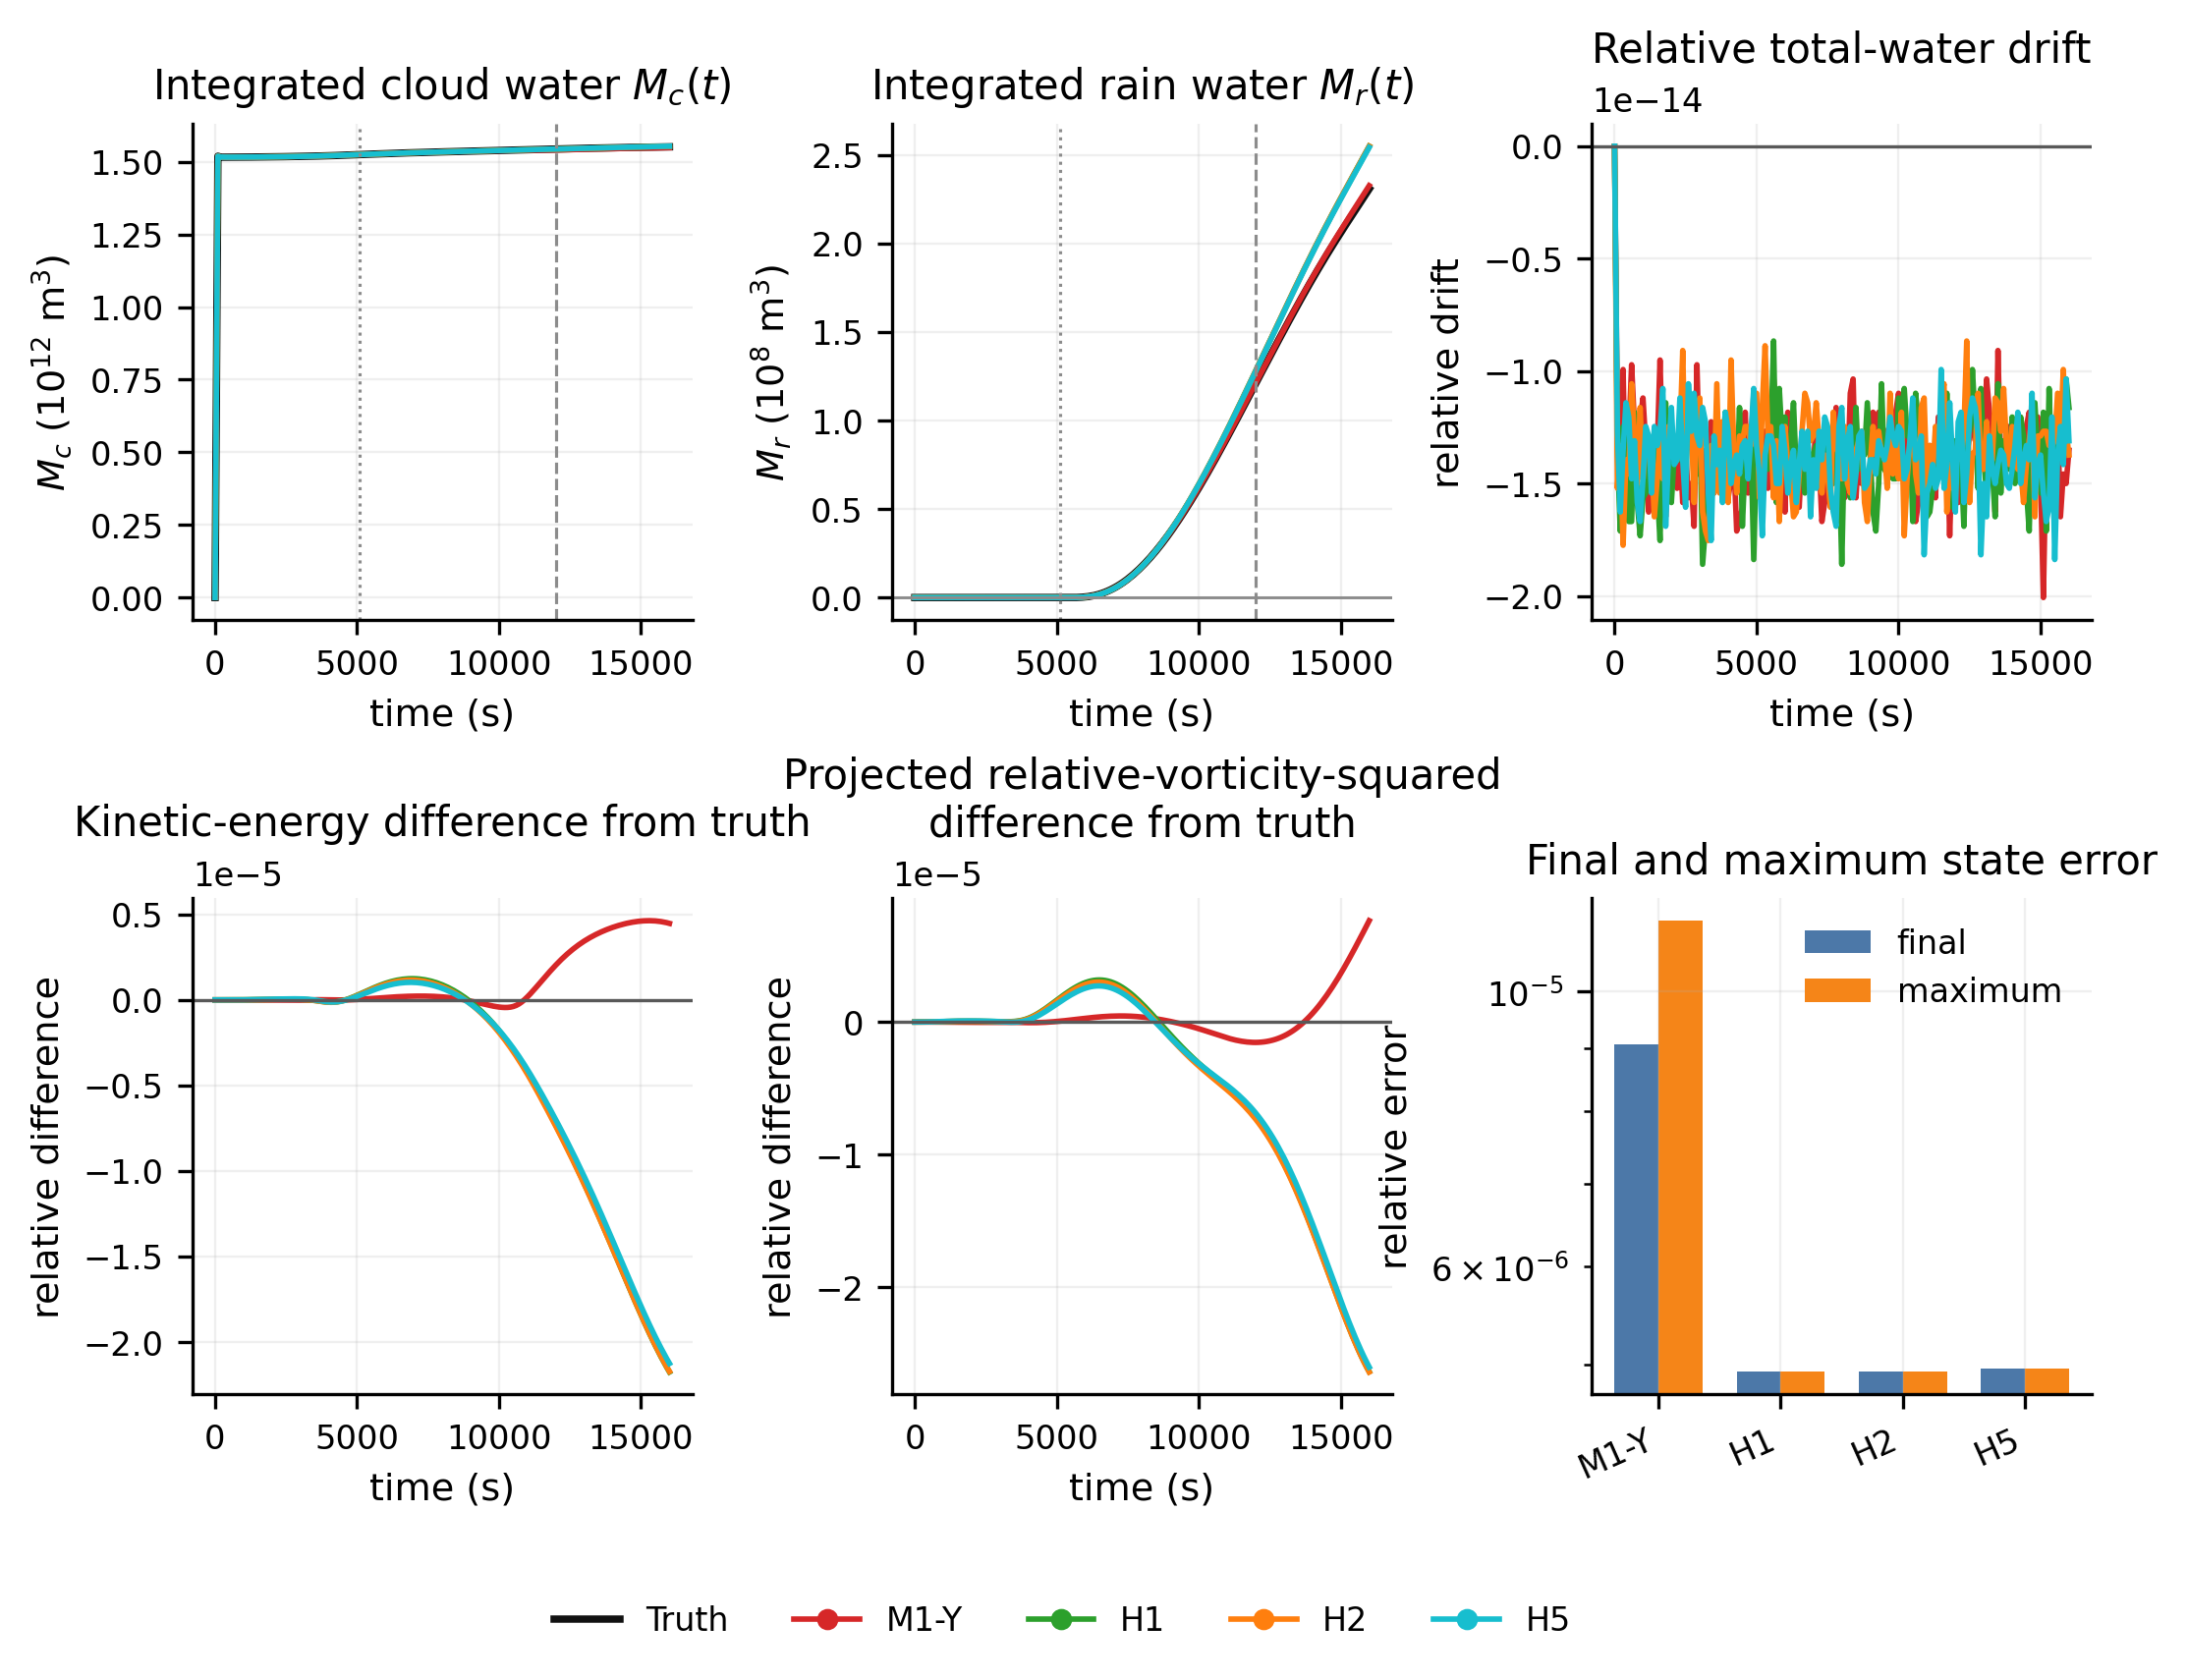
\includegraphics[width=\textwidth]
		{ML5A_main_global_trajectories.png}
		\caption{
			Global evolution of the deployed Representation-A models.
			The panels show integrated cloud water $M_c$, integrated rain water
			$M_r$, relative total-water drift, the difference in kinetic energy
			from truth, the difference in projected relative-vorticity squared from
			truth, and the final and maximum relative state errors.
			The vertical lines indicate first truth rain production and the time of
			peak integrated truth rain production.
			Total-water conservation is imposed by the Representation-A source
			structure.
		}
		\label{fig:ml_global_A}
	\end{figure}
	
Representation B remains numerically stable and also preserves total water to
roundoff, but the rain-water evolution is more sensitive to the training
objective (Fig.~\ref{fig:ml_global_B}). M1-Y slightly overpredicts the final
rain-water reservoir but remains closest to the truth, whereas H1, H2, and H5
underpredict it. This behavior is consistent with the local-physics results
above: M1-Y provides the most accurate approximation of the analytical rain
rate $R$, while the state-based models tolerate substantially larger local
errors in $R$ while still maintaining small overall state errors. The
kinetic-energy and vorticity diagnostics remain close to truth for all four
models. Thus an accurate global state trajectory does not require equally
accurate recovery of each individual local moist-process rate.
	
	\begin{figure}[h!]
		\centering
		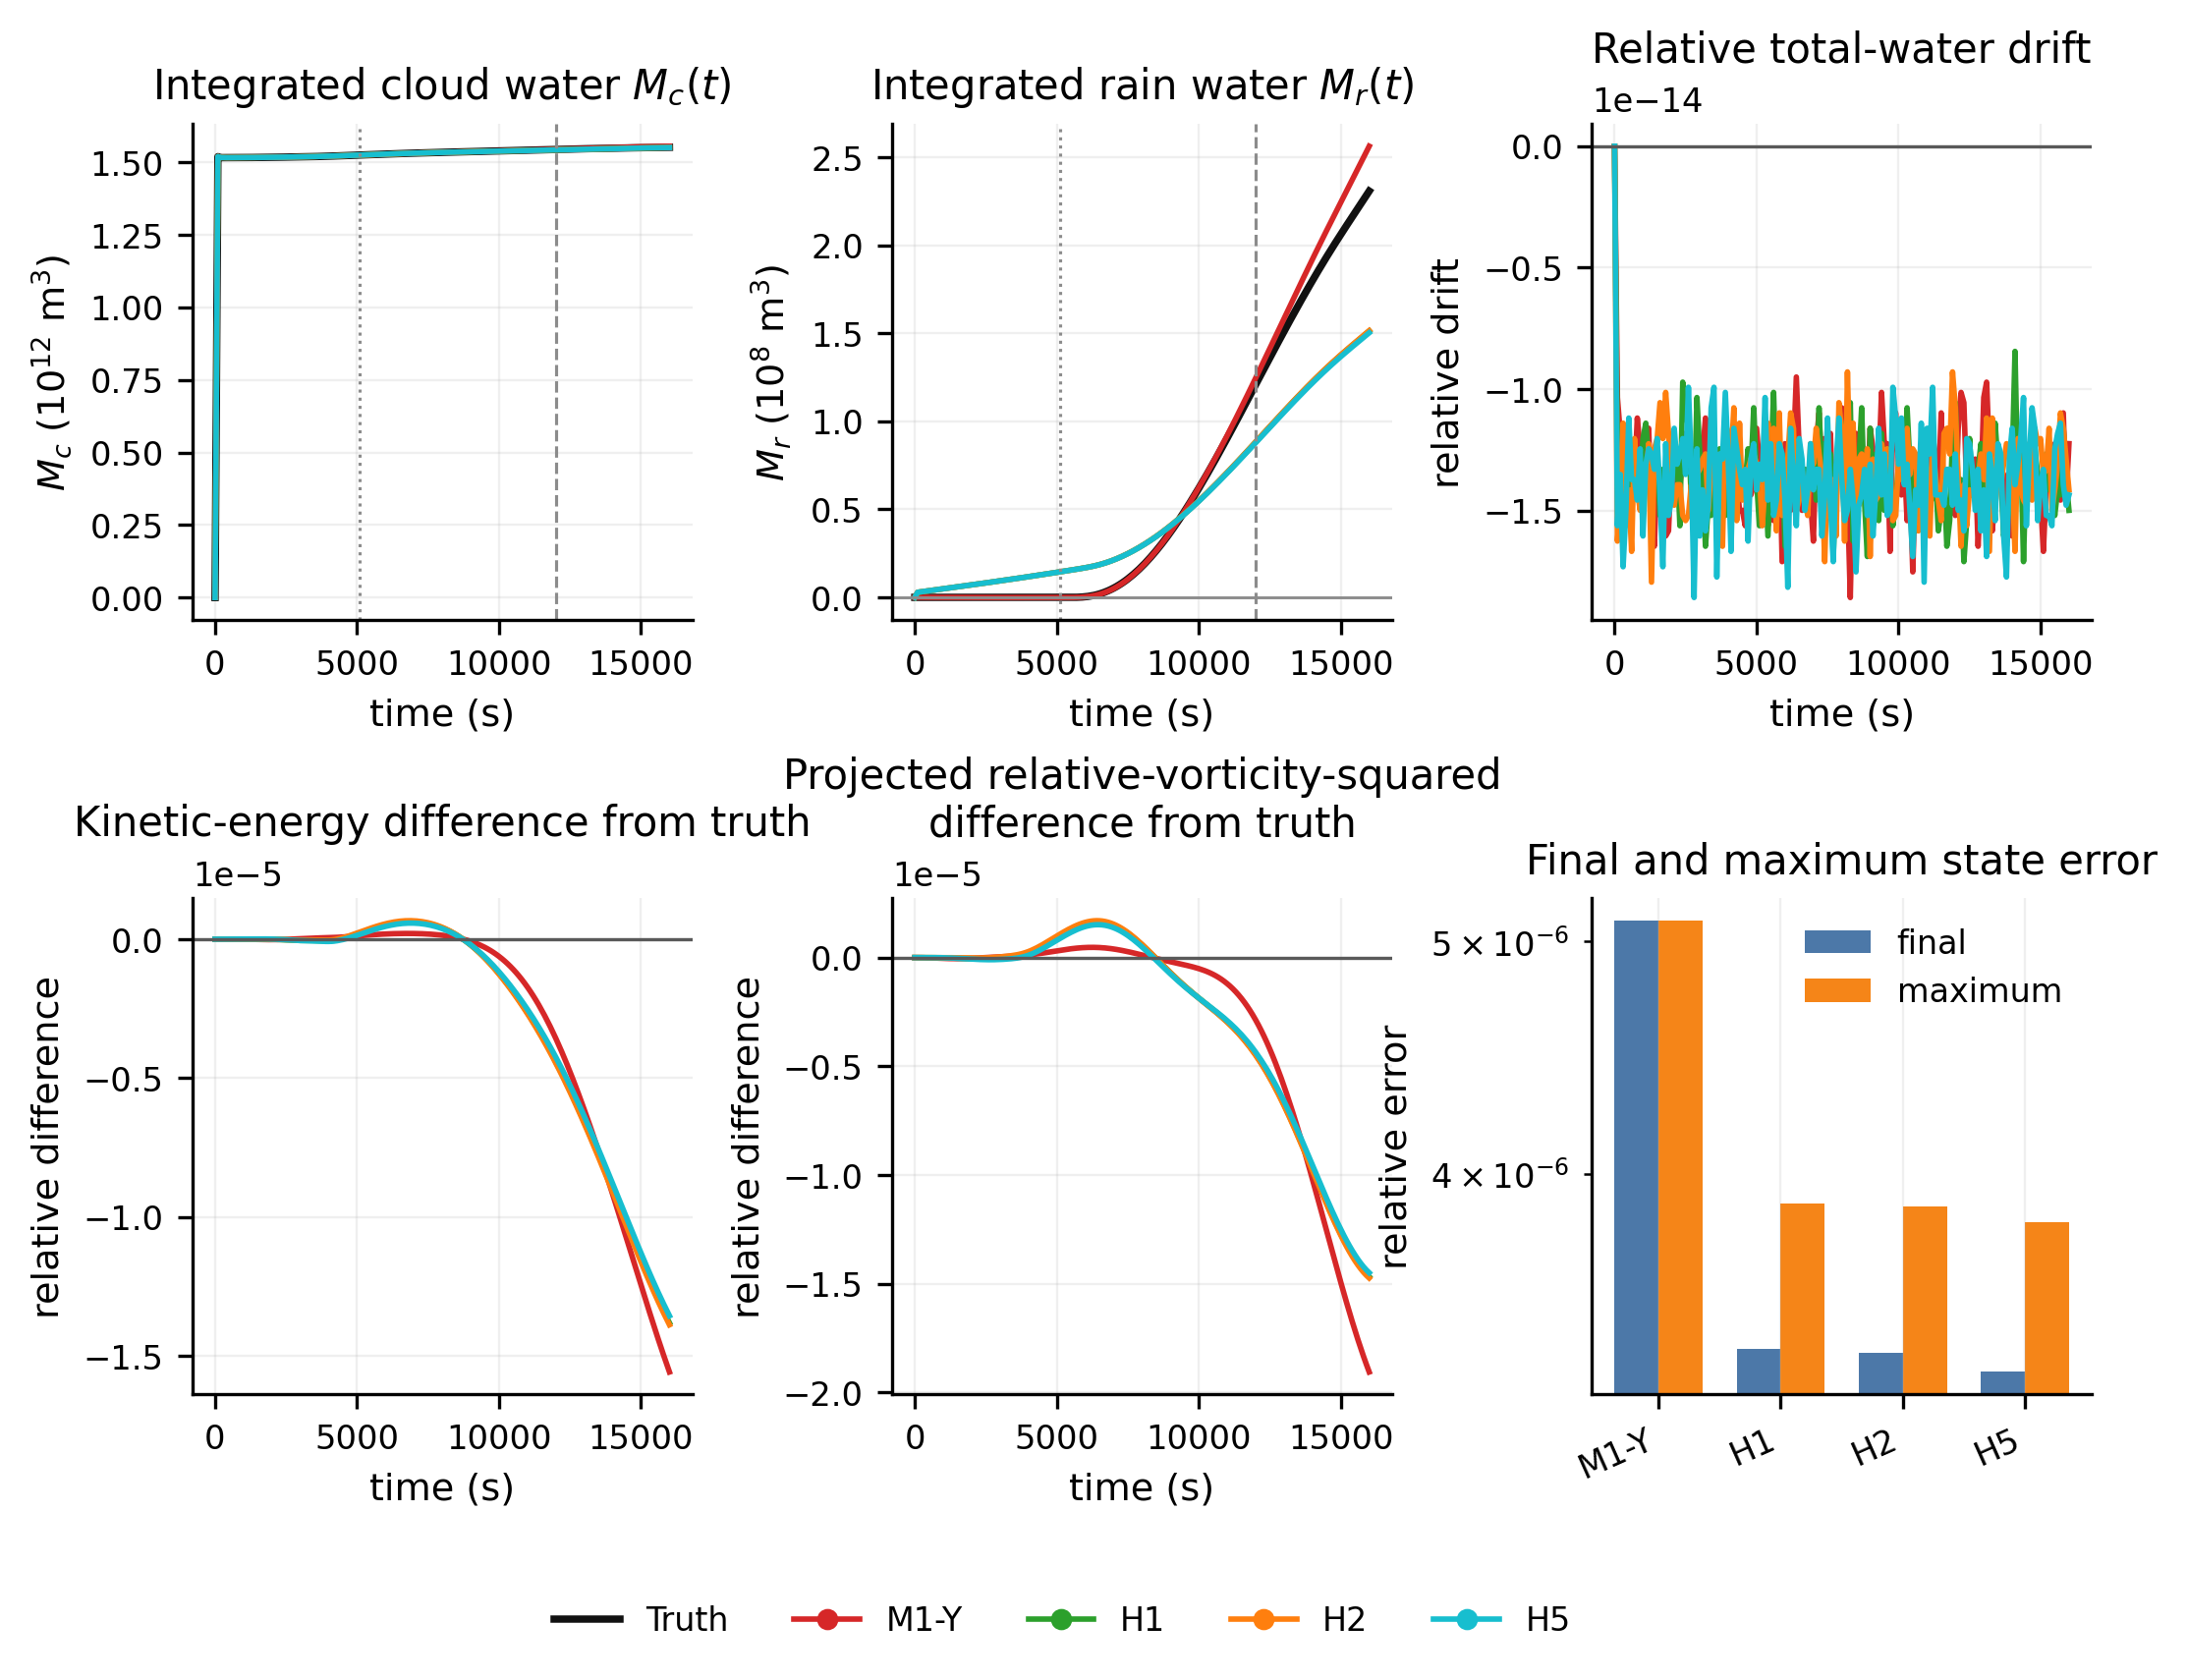
\includegraphics[width=\textwidth]
		{ML5B_main_global_trajectories.png}
		\caption{
			Global evolution of the deployed Representation-B models.
			The panels show integrated cloud water $M_c$, integrated rain water
			$M_r$, relative total-water drift, the difference in kinetic energy
			from truth, the difference in projected relative-vorticity squared from
			truth, and the final and maximum relative state errors.
			Representation B learns both $A$ and $R$ while retaining the prescribed
			moist-source structure, so total-water conservation remains enforced
			algebraically.
		}
		\label{fig:ml_global_B}
	\end{figure}
	
Representation C behaves qualitatively differently
(Fig.~\ref{fig:ml_global_C}). M1-Y remains comparatively close to the truth,
although its water partition and total-water conservation are less accurate
than in the structured representations. The H1, H2, and H5 models
progressively depart from the physical solution. Cloud water is increasingly
underestimated, while the predicted rain-water reservoir becomes negative and
its magnitude grows during the simulation. These models also develop
substantial total-water drift and considerably larger errors in the
kinetic-energy and relative-vorticity-squared diagnostics. The final state
error increases from M1-Y through H1, H2, and H5.

This behavior is notable because the H2 and H5 training errors decrease during
their respective optimization stages (Fig.~\ref{fig:ml_optimization}), while
the error after the full 160-step deployed simulation increases. Thus, for
Representation C, improving the model over the two- and five-step training
windows does not lead to a more accurate long-time solution. Because H2 and H5
were each optimized for only 20 iterations, however, the present calculations
do not determine whether additional optimization would alter this behavior.

The Representation-C results demonstrate the importance of distinguishing
trajectory optimization from physical structure. Because the four moist-source
components are predicted independently, neither water conservation nor the
physical cloud--rain partition is guaranteed. The H1, H2, and H5 sequence
does not recover these relationships and, for the present case, produces a
numerically well-defined but progressively less physical evolution.
	
	\begin{figure}[h!]
		\centering
		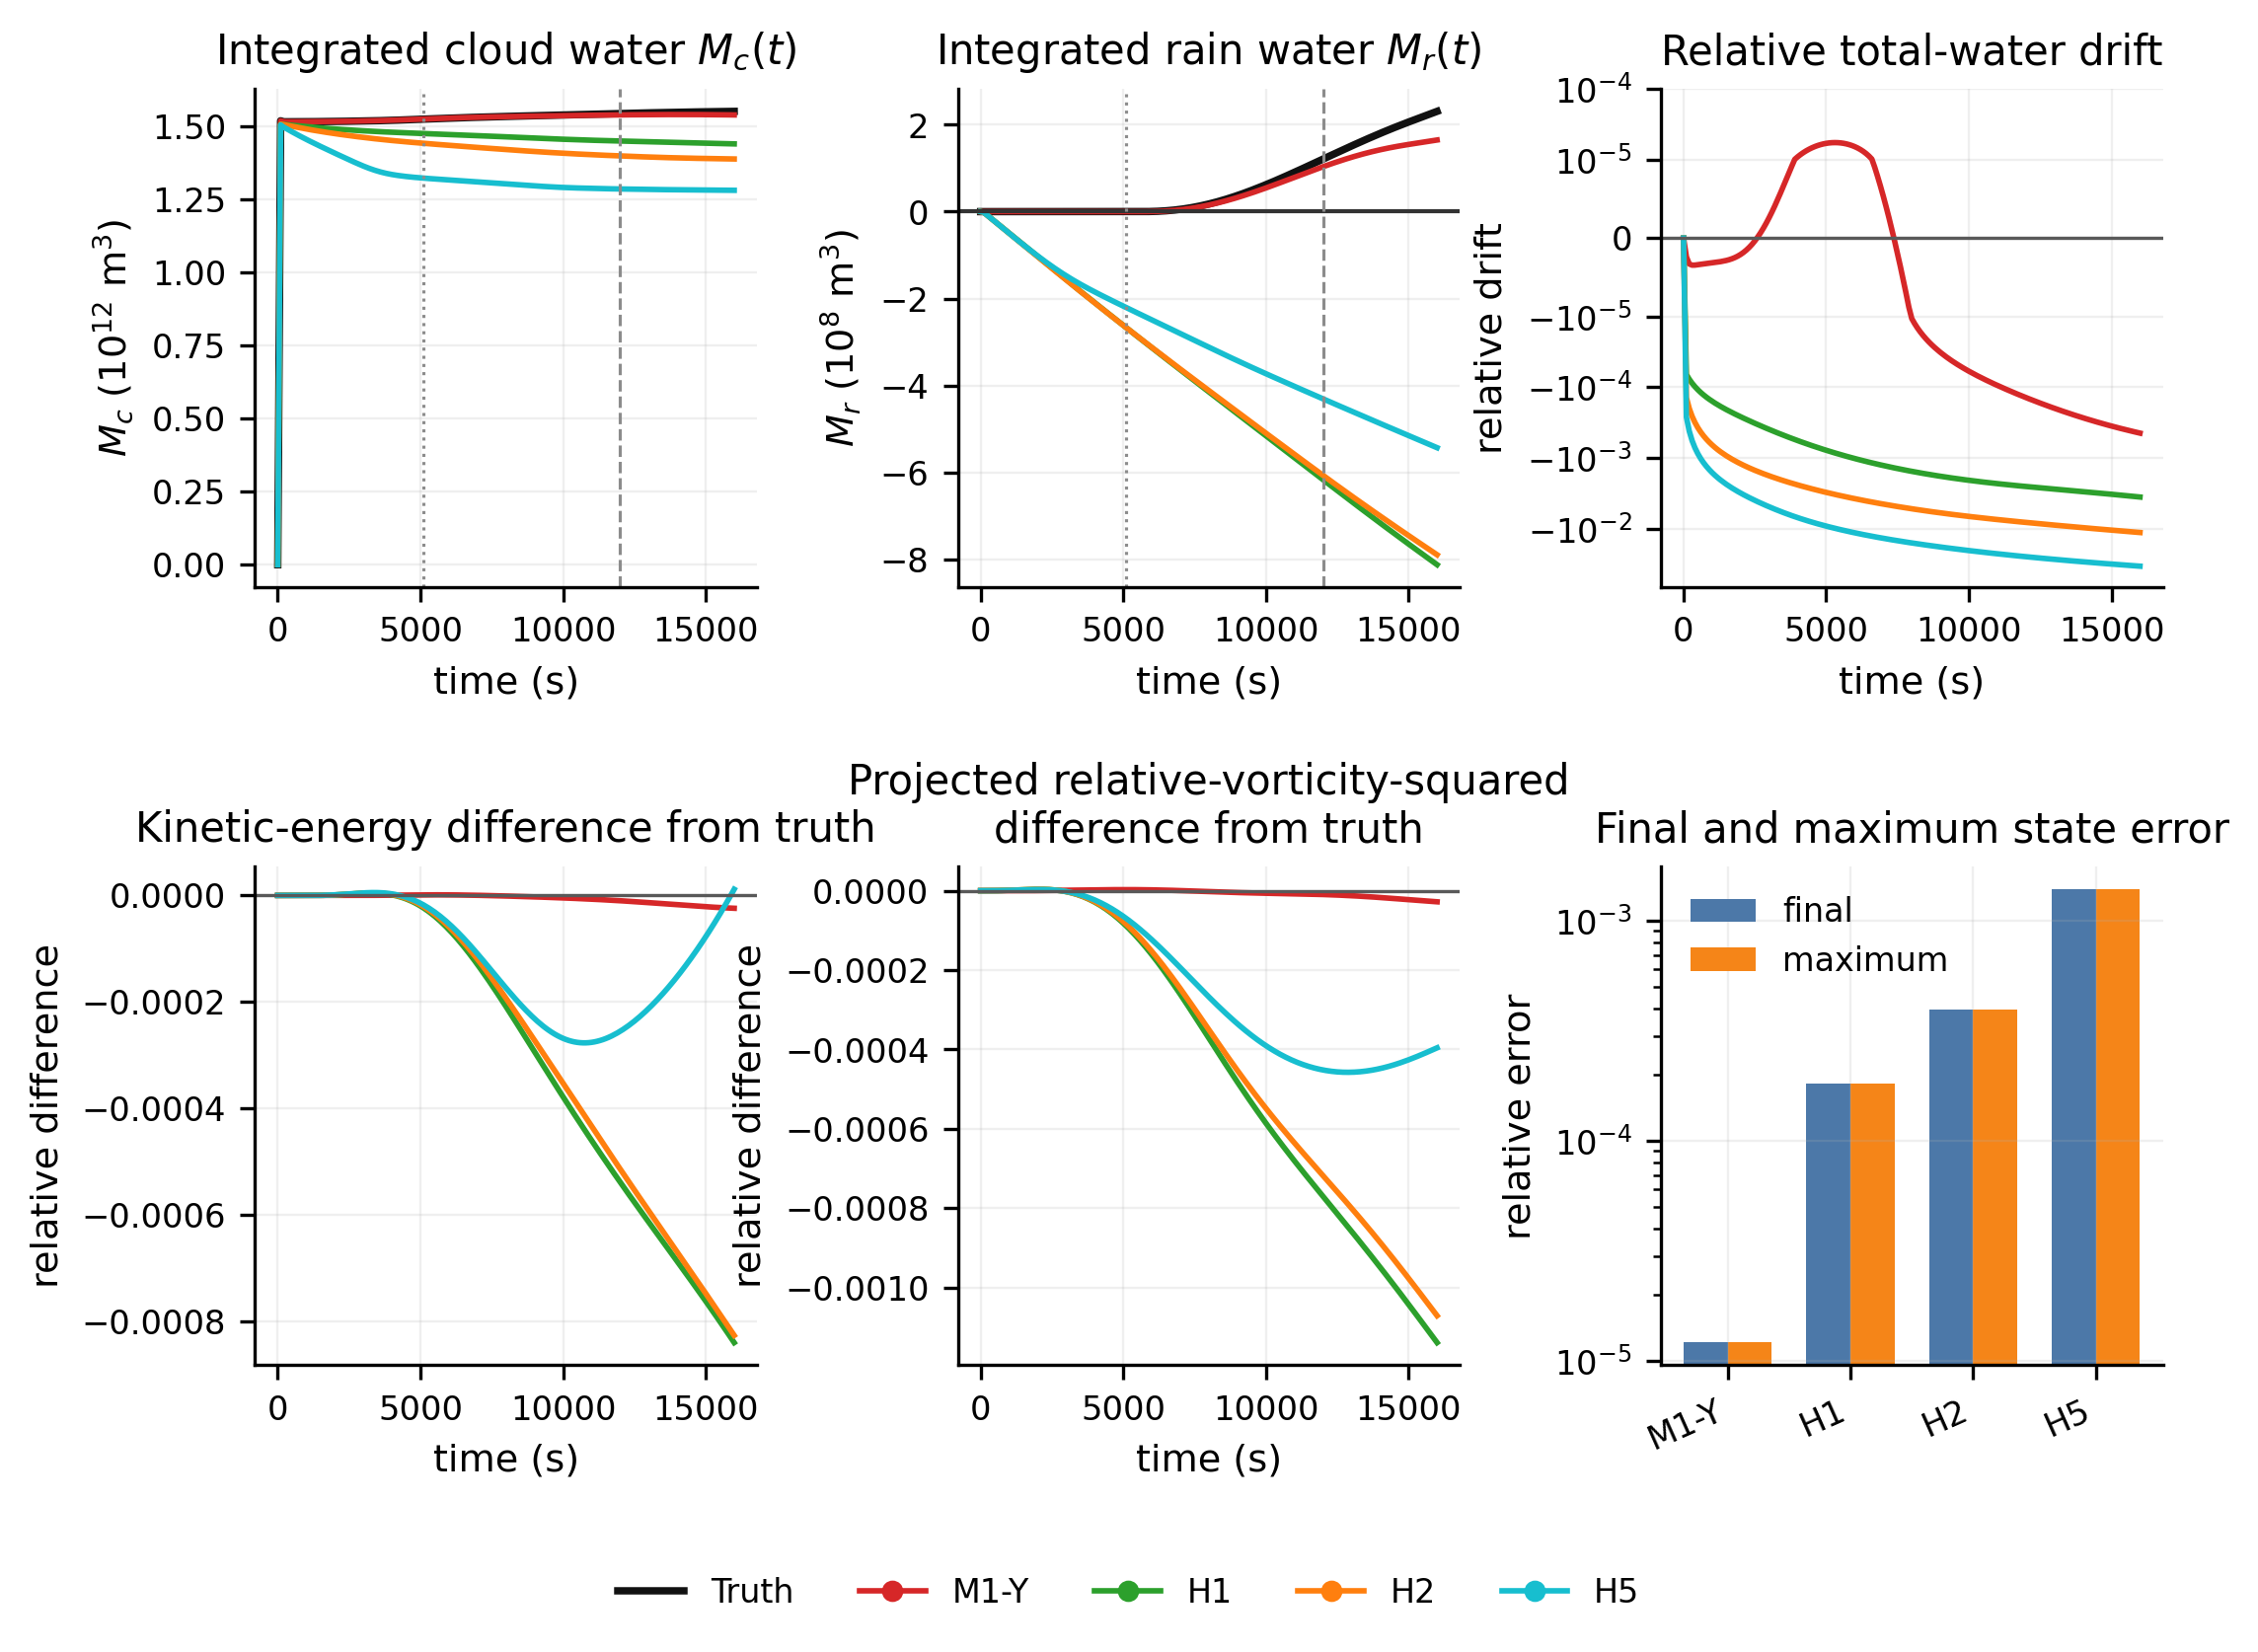
\includegraphics[width=\textwidth]
		{ML5C_main_global_trajectories.png}
		\caption{
			Global evolution of the deployed Representation-C models.
			The panels show integrated cloud water $M_c$, integrated rain water
			$M_r$, relative total-water drift, the difference in kinetic energy
			from truth, the difference in projected relative-vorticity squared from
			truth, and the final and maximum relative state errors.
			Unlike Representations A and B, Representation C predicts the four
			moist-source components independently and does not impose total-water
			conservation or the analytical cloud--rain source structure.
			The horizontal zero line in the rain-water panel highlights the
			negative rain water produced by several of the state-based models.
		}
		\label{fig:ml_global_C}
	\end{figure}
	
	\section{Deployed Hybrid Dynamics}\label{sec:HybridSims}	 
	 The preceding section quantified the deployed models using local errors,
	 conservation diagnostics, and domain-integrated trajectories. We now illustrate
	 the evolution of corresponding moisture fields. All truth and learned-model plots use the same five
	 reference times and the same color limits for each variable.
	 
\subsection{Truth}

Figure~\ref{fig:hybrid_truth_reference} provides the common truth reference.
The columns correspond to $t=0$, $5000$, $6100$, $12000$, and
$16000~\mathrm{s}$. The rows show relative humidity, specific cloud water
$q_c$, specific rain water $q_r$, and rain-production rate $R$.
Gray contours indicate relative vorticity. 

\begin{figure}[p]
	\centering
	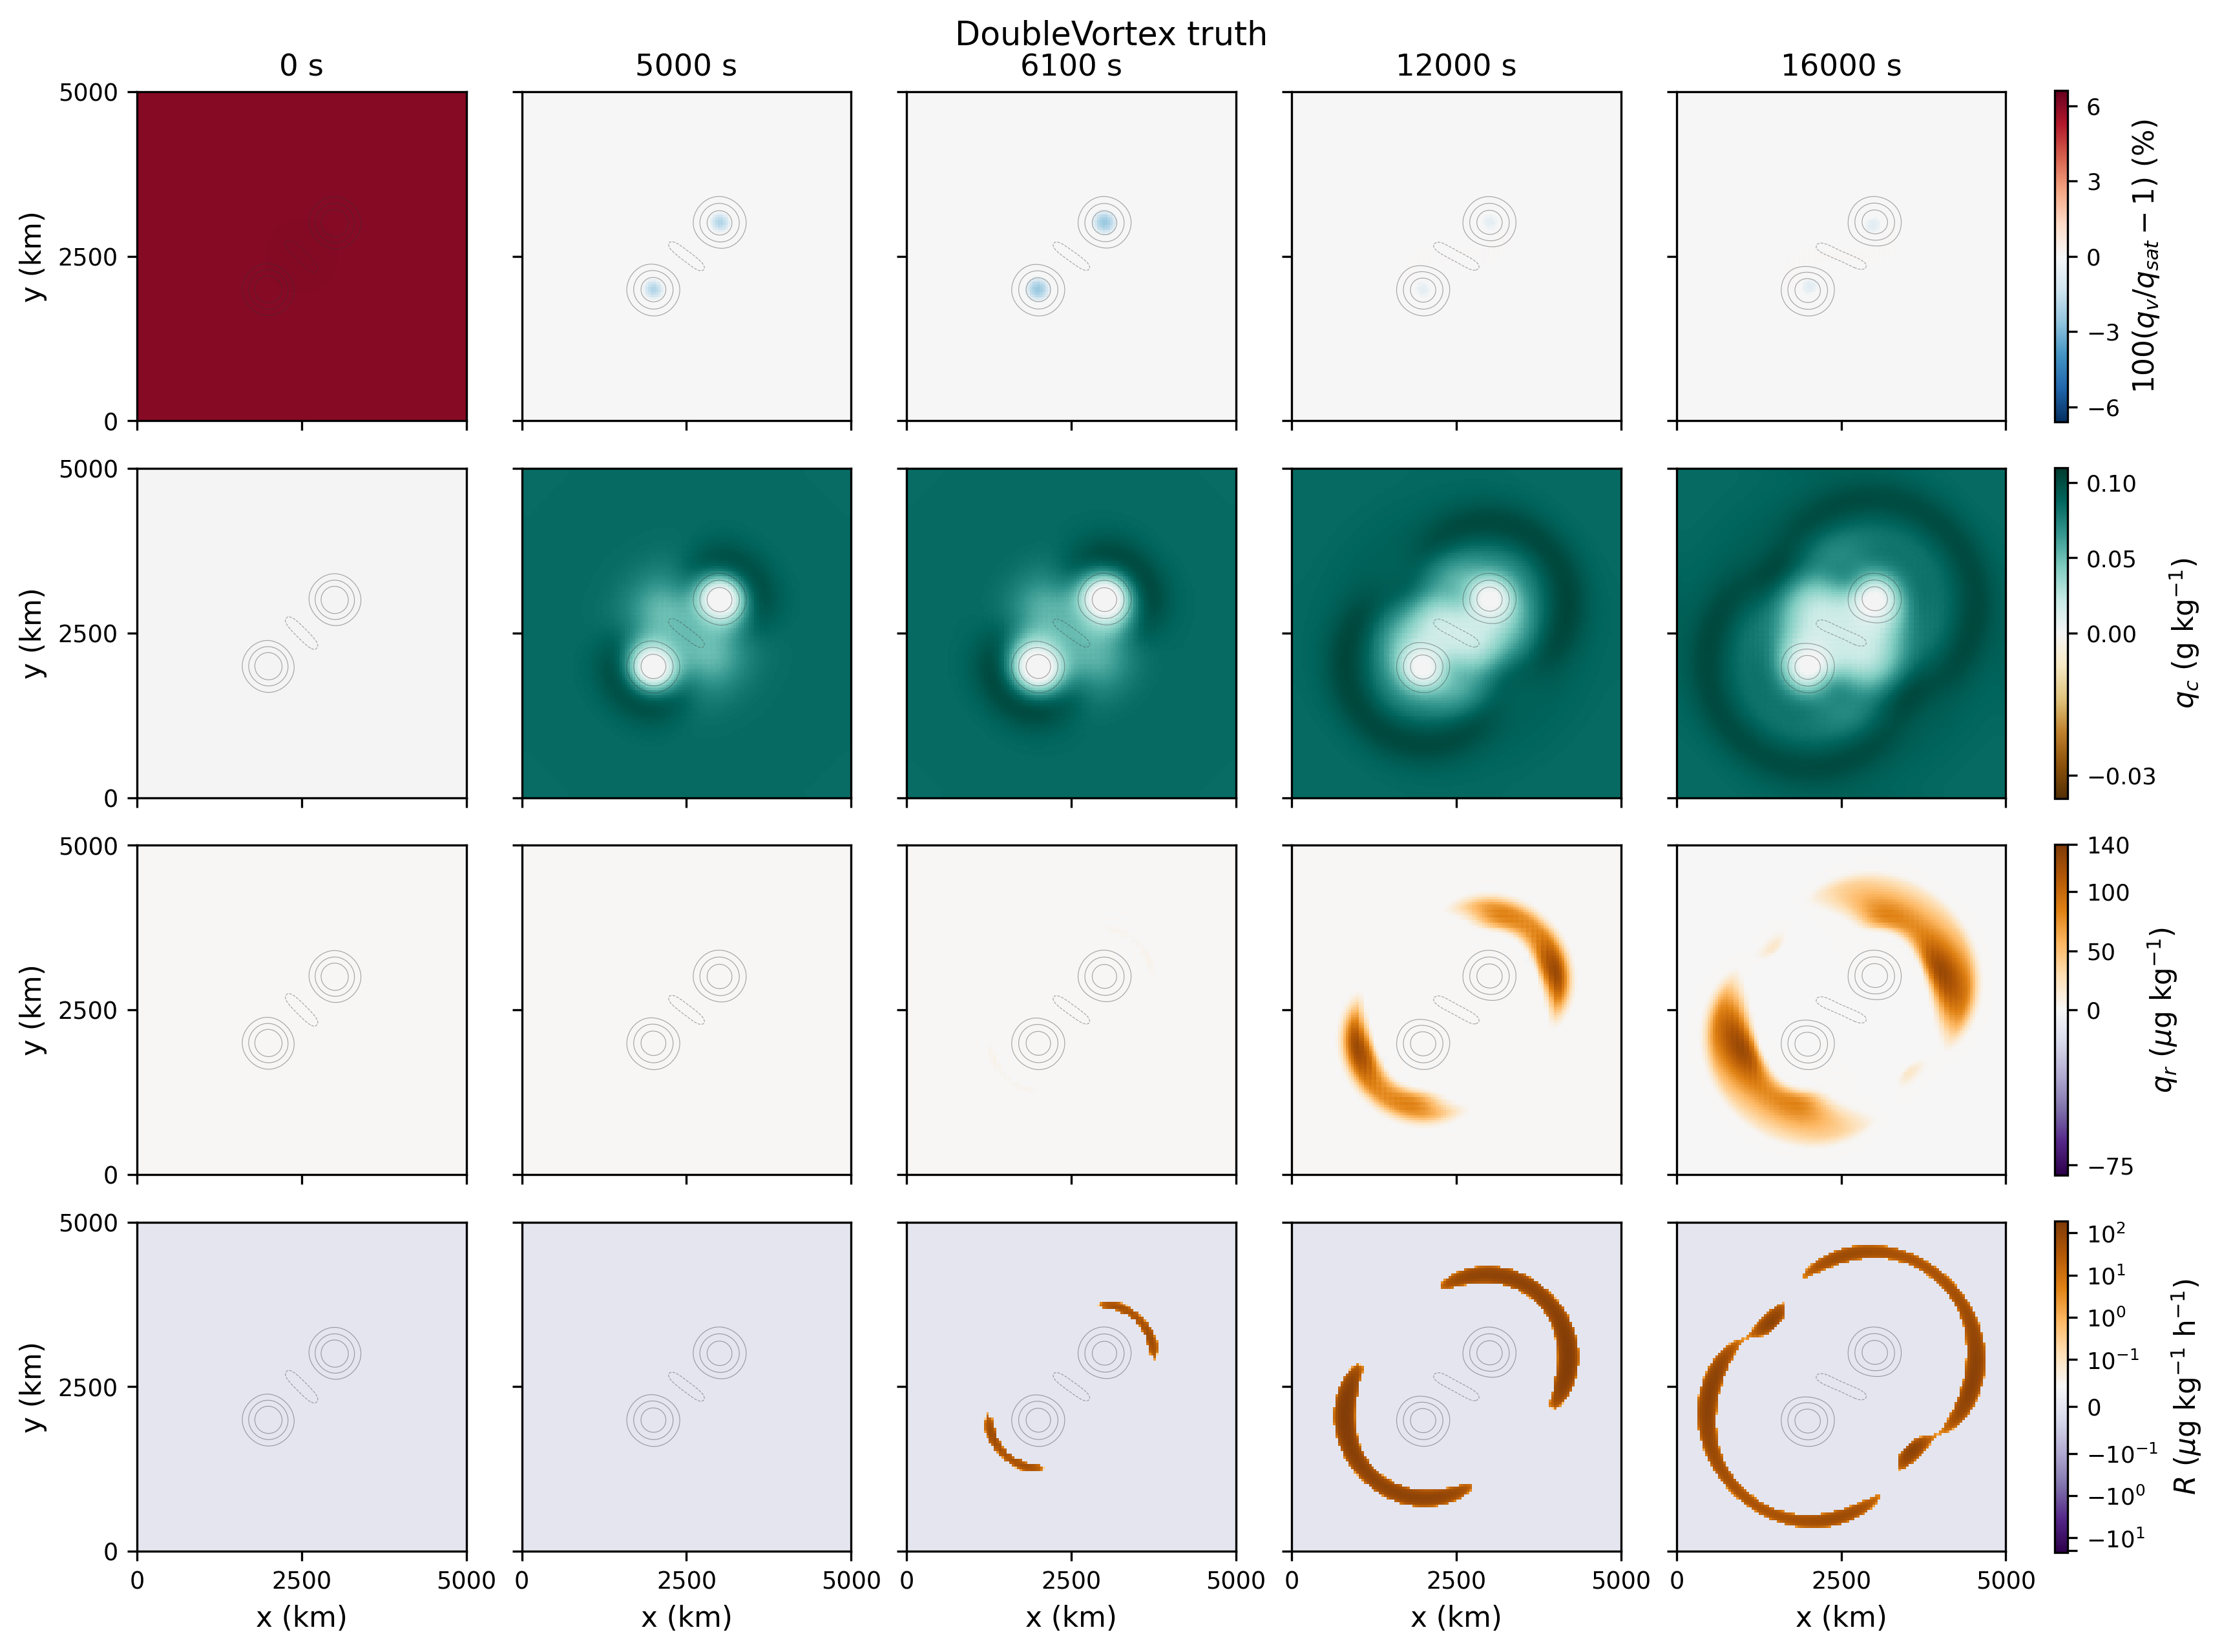
\includegraphics[width=\textwidth]
	{gallery_truth_reference_common_scale.png}
	\caption{
		Common spatial reference for the ground-truth DoubleVortex evolution.
		Columns show $t=0$, $5000$, $6100$, $12000$, and $16000~\mathrm{s}$.
		Rows show saturation departure $100(q_v/q_{\mathrm{sat}}-1)$,
		specific cloud water $q_c$, specific rain water $q_r$, and the
		analytical rain-production rate $R$, respectively.
		Gray contours show relative vorticity.
		The same color limits, spatial coordinates, and vorticity contour levels
		are used in all deployed-model galleries.
	}
	\label{fig:hybrid_truth_reference}
\end{figure}

\clearpage


\subsection{Representation A}

The deployed evolution is robust across all four training objectives illustrated across figures \ref{fig:hybrid_A_M1Y} to \ref{fig:hybrid_A_H5}. The two-vortex structure is preserved and the
location and overall shape of the cloud and rain bands is close to that in the truth
solution. Minute differences arise in amplitude and in the detailed
late-time relative humidity and rain-production fields. Overall, these spatial
results are consistent with the small state and water-partition errors found
in Sec.~\ref{sec:MLResults}.

\begin{figure}[p]
	\centering
	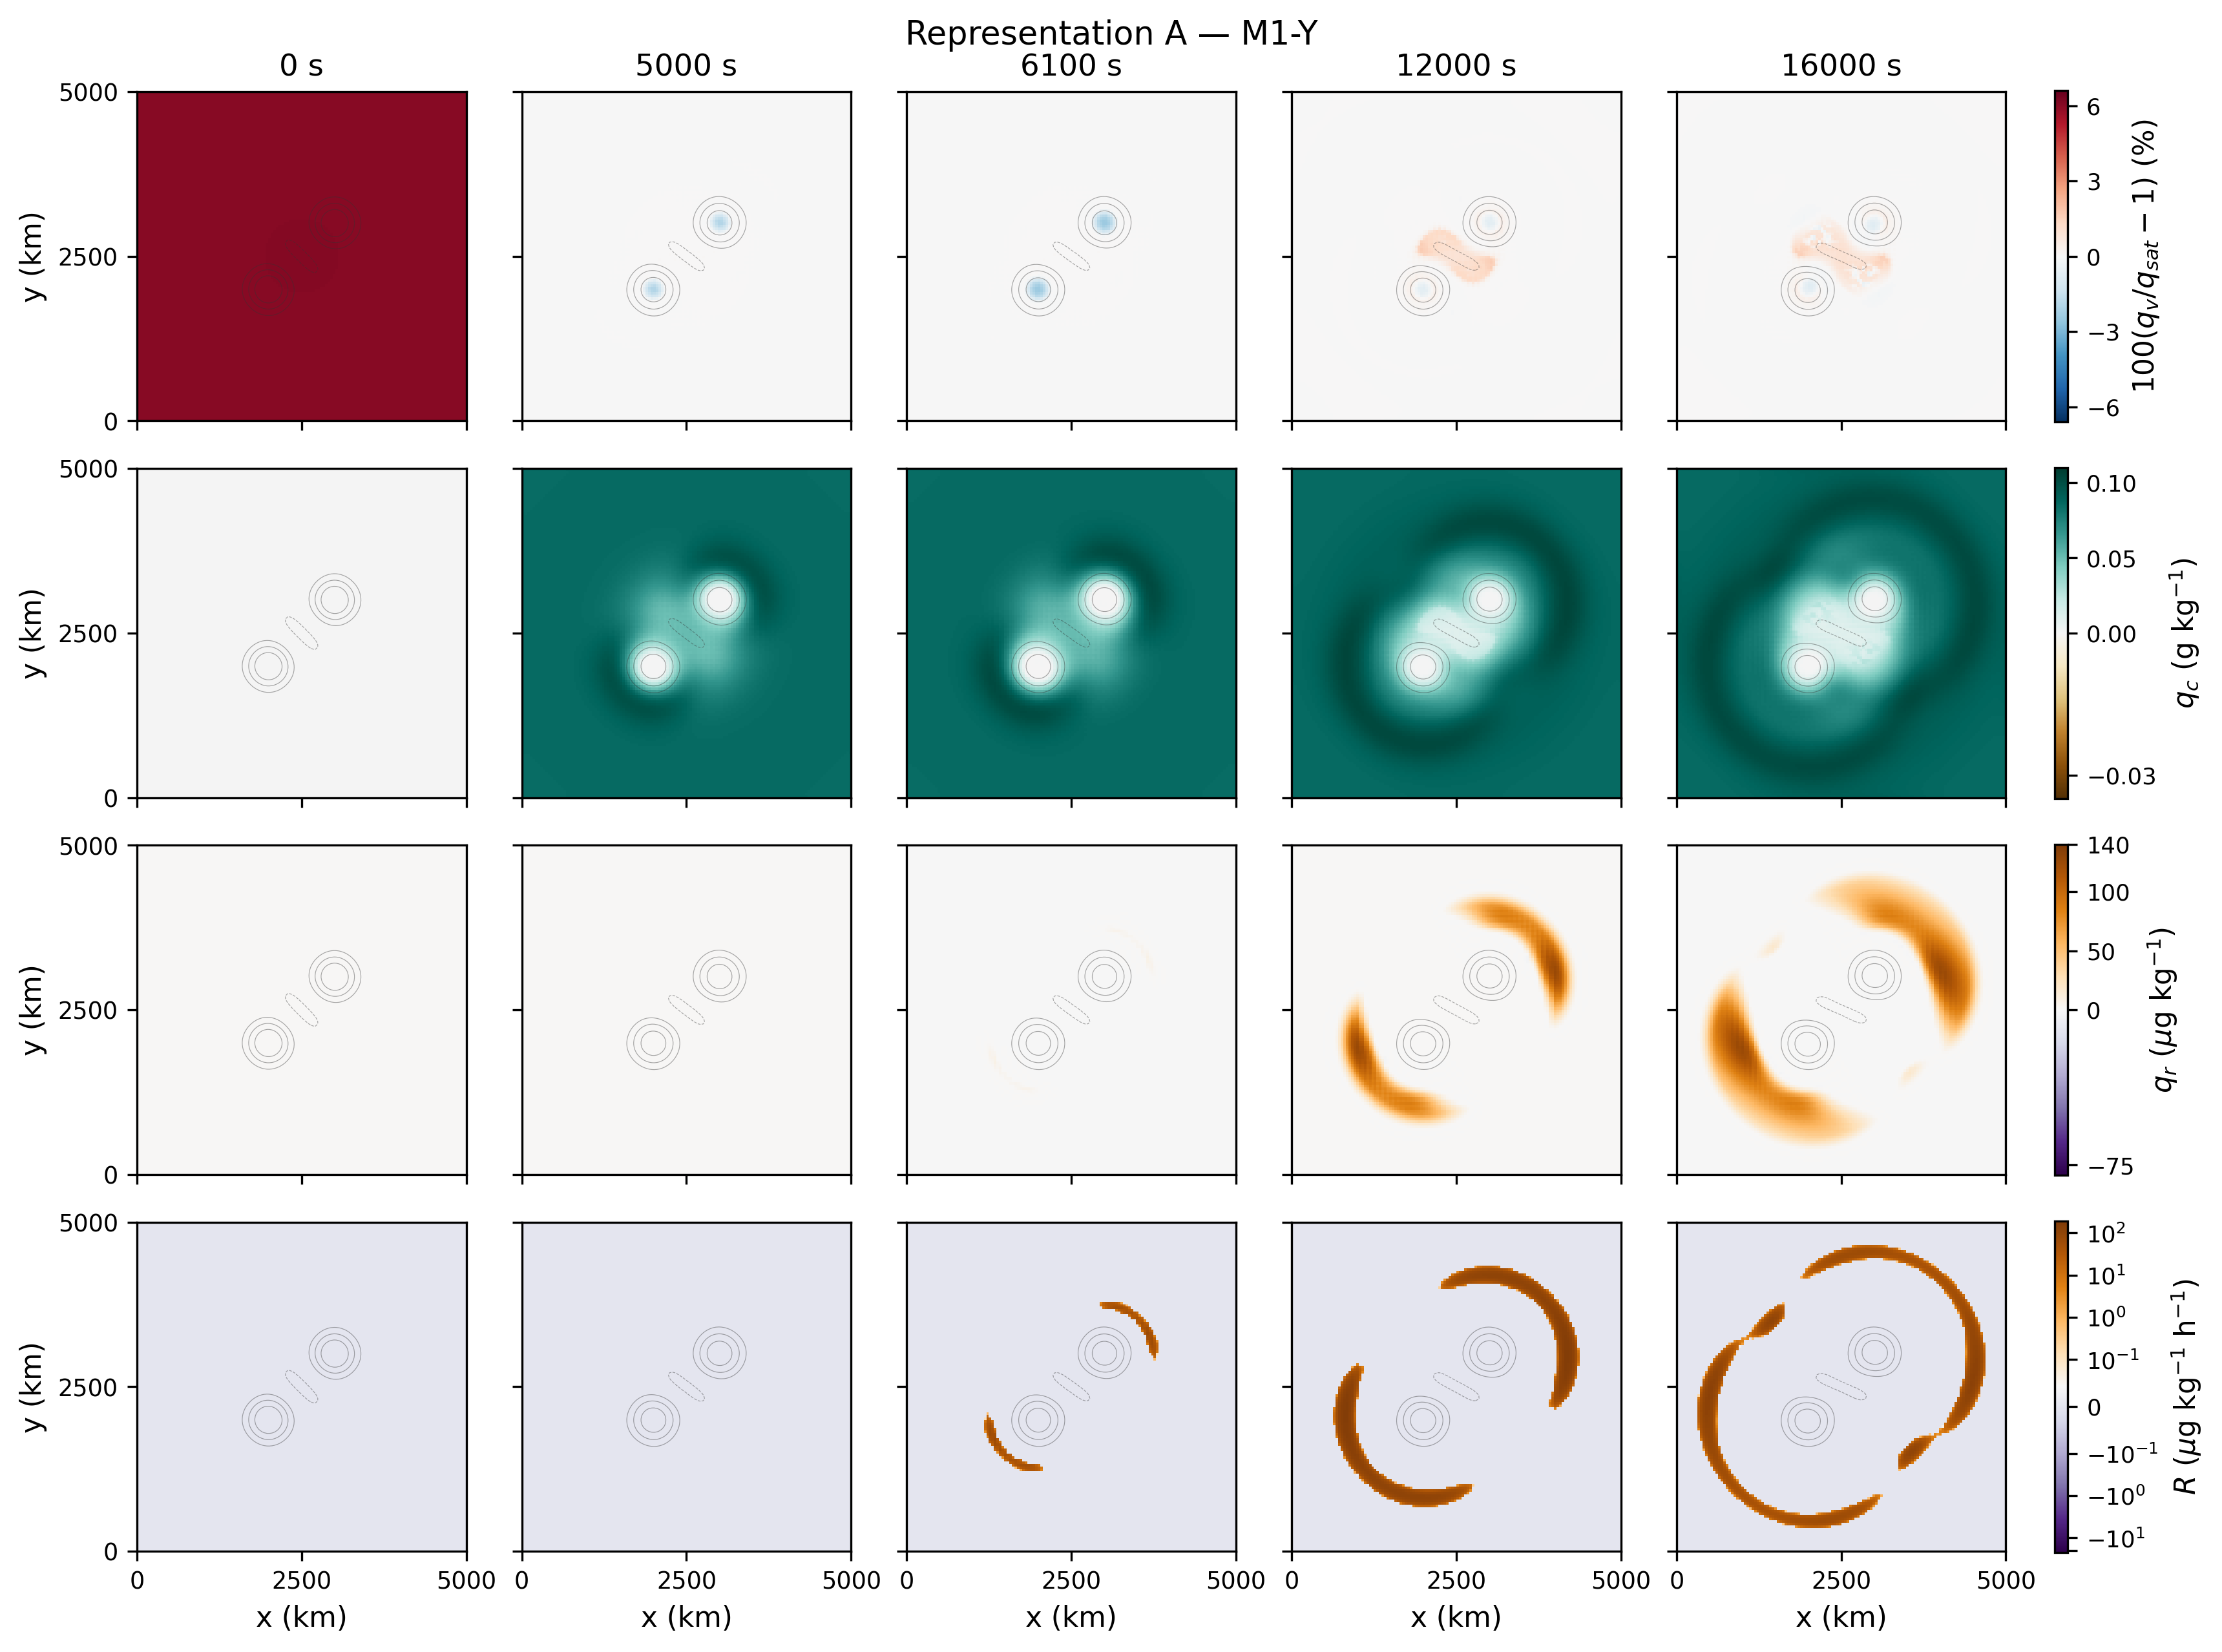
\includegraphics[width=\textwidth]{gallery_repA_M1Y.png}
	\caption{Same as figure \ref{fig:hybrid_truth_reference} but for Representation-A evolution using M1-Y.}
	\label{fig:hybrid_A_M1Y}
\end{figure}

\begin{figure}[p]
	\centering
	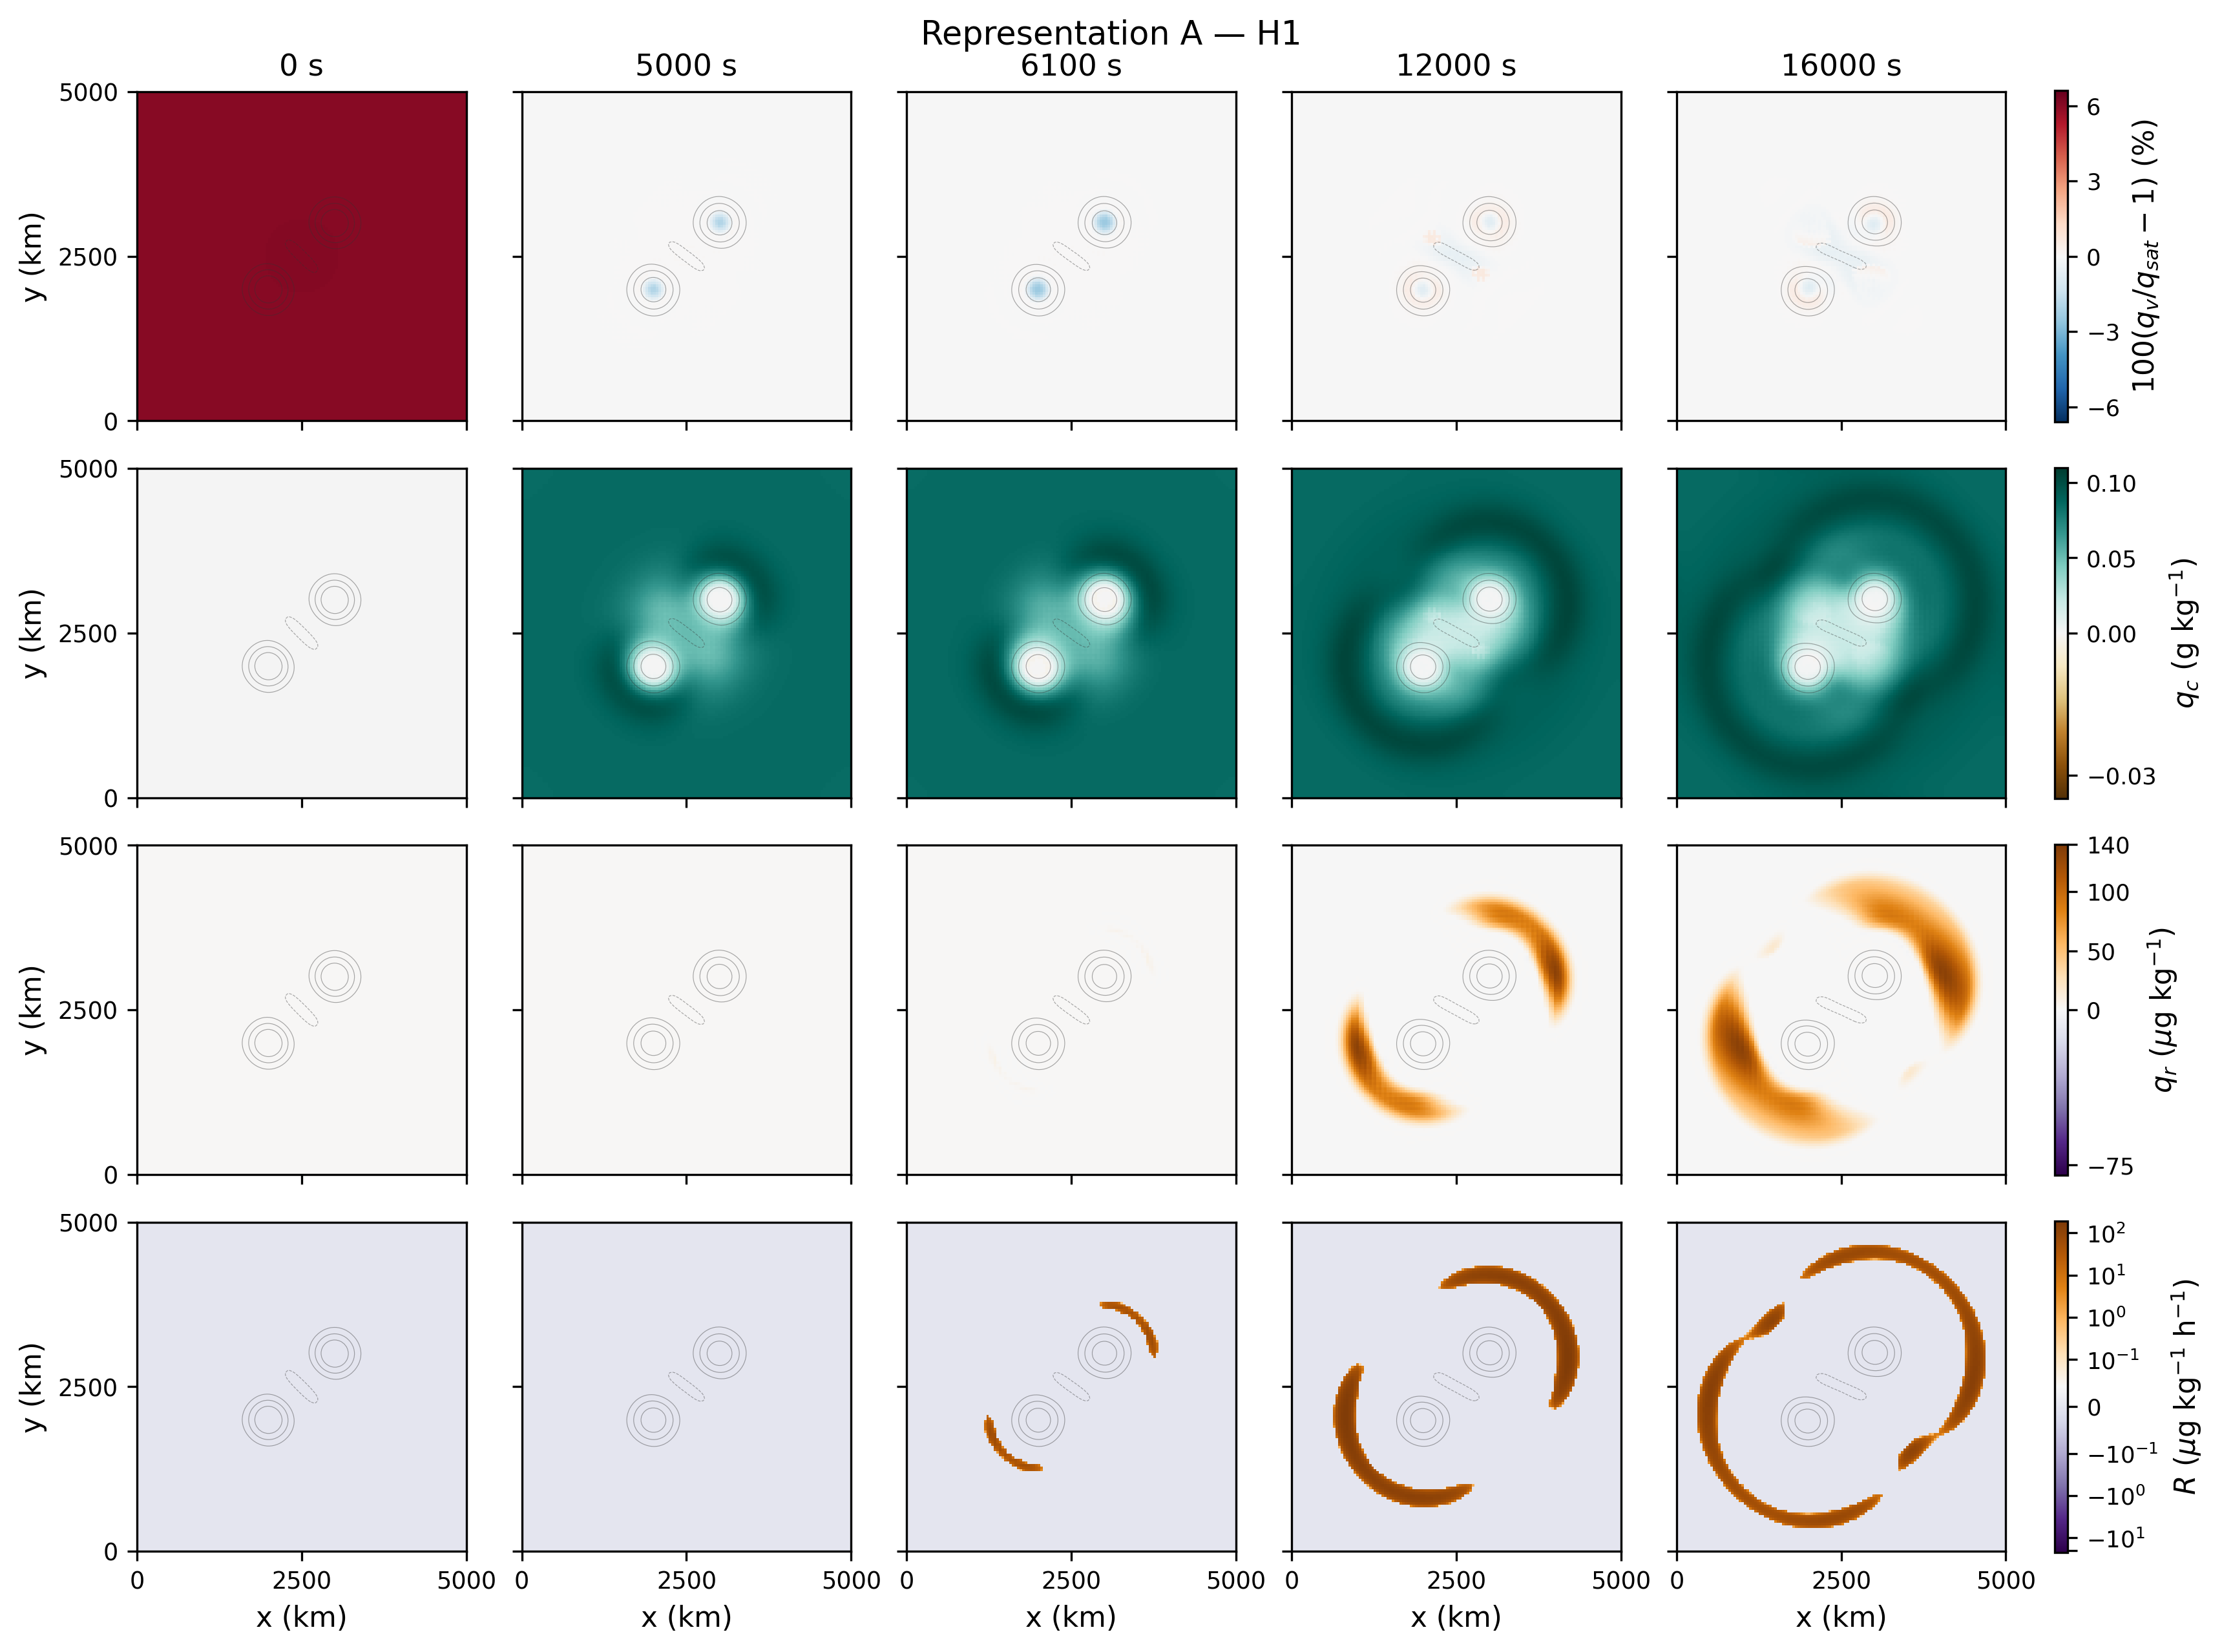
\includegraphics[width=\textwidth]{gallery_repA_H1.png}
	\caption{Same as figure \ref{fig:hybrid_truth_reference} but for Representation-A evolution using H1/M2-Y.}
	\label{fig:hybrid_A_H1}
\end{figure}

\begin{figure}[p]
	\centering
	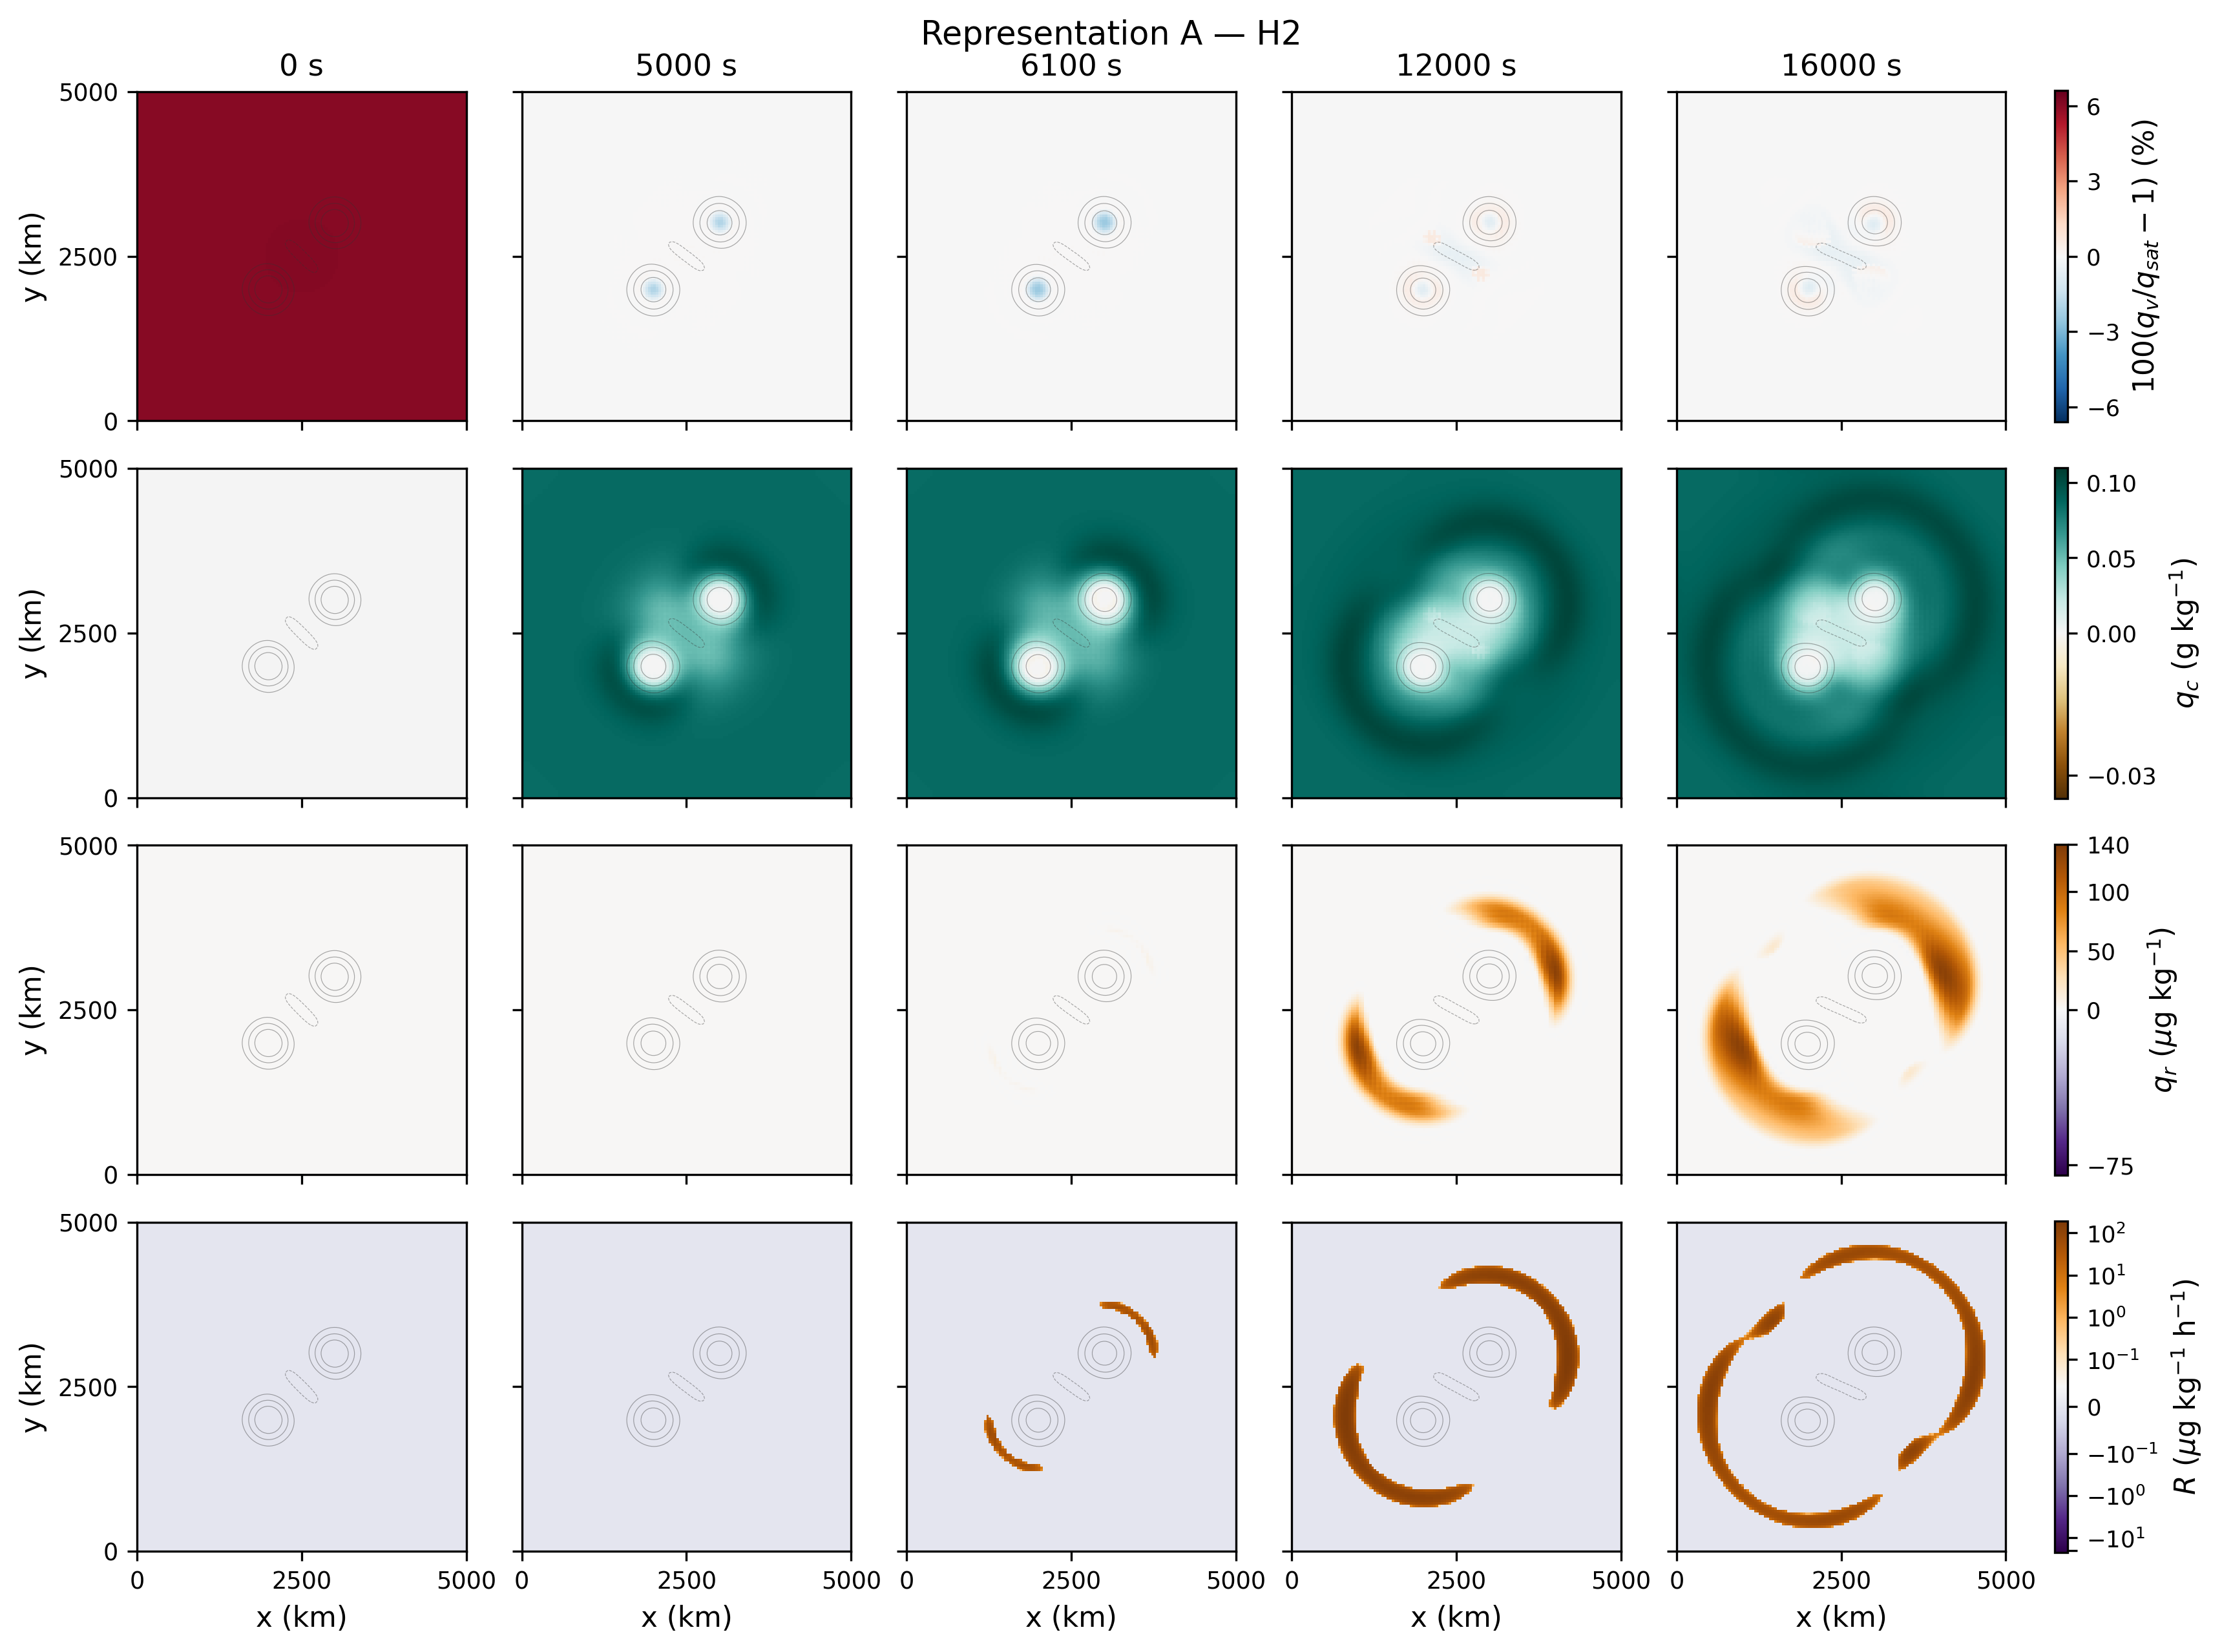
\includegraphics[width=\textwidth]{gallery_repA_H2.png}
	\caption{Same as figure \ref{fig:hybrid_truth_reference} but for Representation-A evolution using H2.}
	\label{fig:hybrid_A_H2}
\end{figure}

\begin{figure}[p]
	\centering
	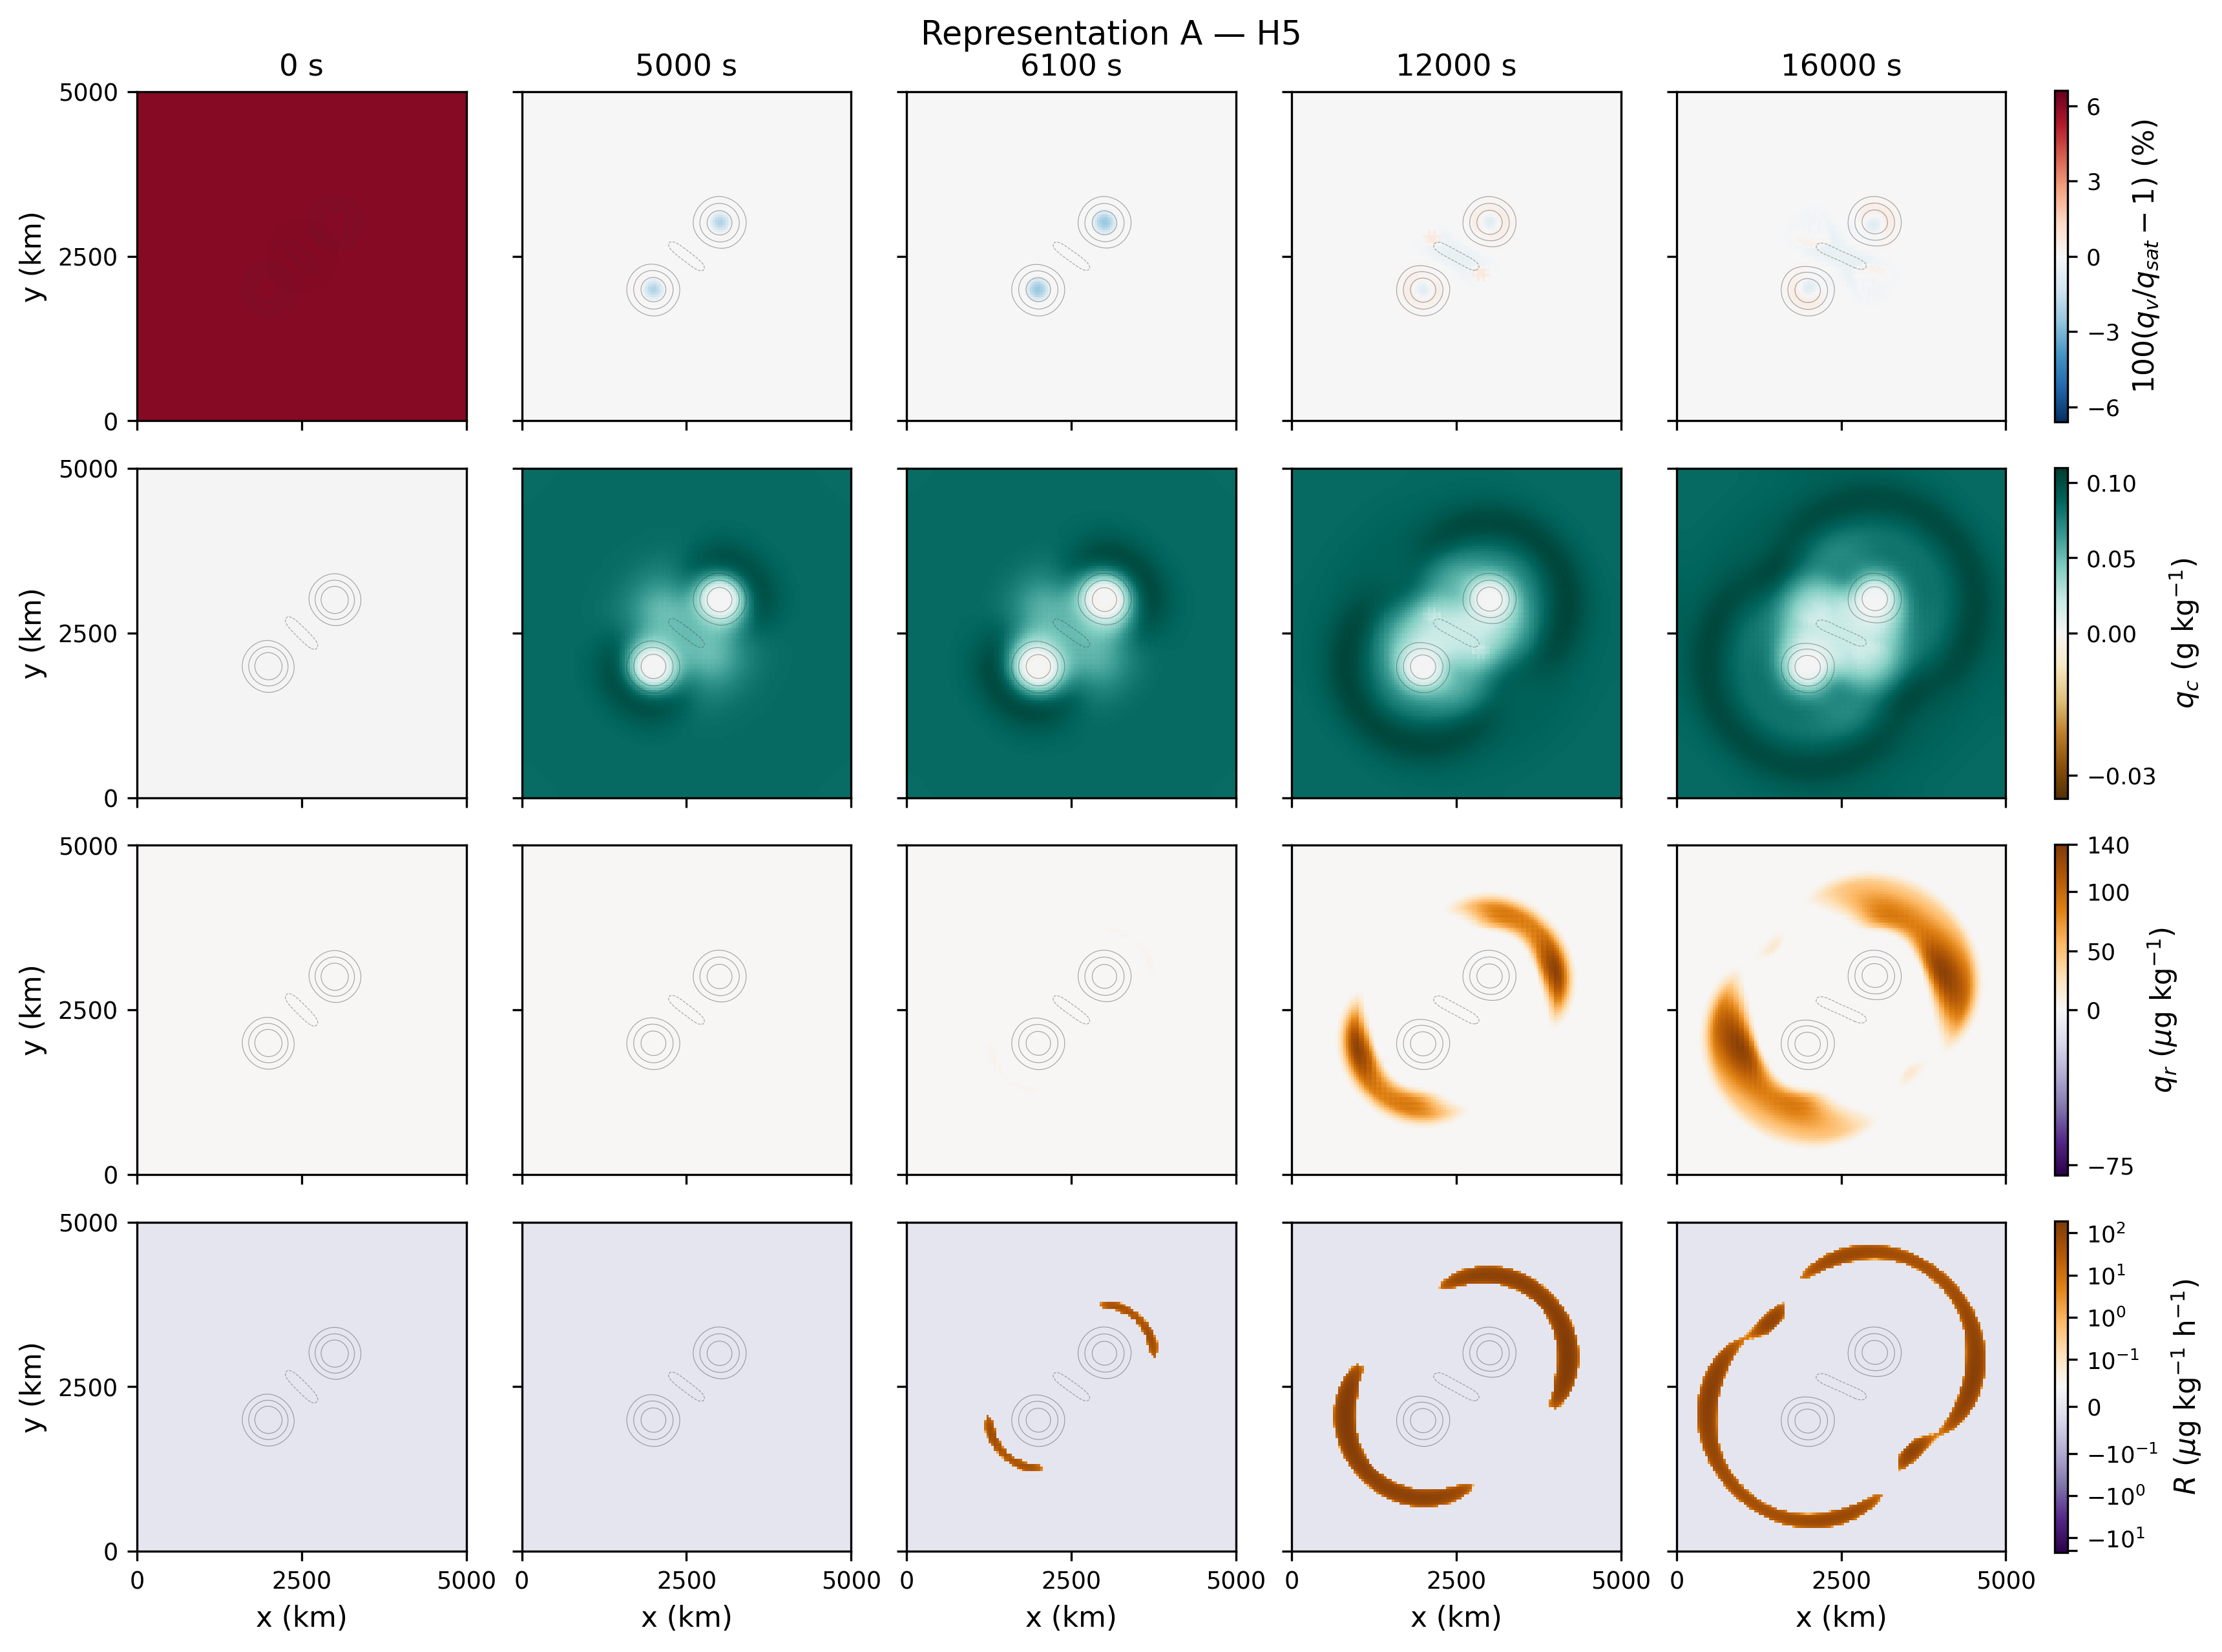
\includegraphics[width=\textwidth]{gallery_repA_H5.png}
		\caption{Same as figure \ref{fig:hybrid_truth_reference} but for Representation-A evolution using H5.}
	\label{fig:hybrid_A_H5}
\end{figure}

\clearpage


\subsection{Representation B}

Representation B also preserves the principal spatial structure of the
solution. The vortex skeleton, cloud envelope, and locations of the two rain
bands remain close to truth for all four training objectives. M1-Y produces
rain-water bands closest to the truth (figure \ref{fig:hybrid_B_M1Y}),
whereas H1 (figure \ref{fig:hybrid_B_H1}), H2(figure \ref{fig:hybrid_B_H2}), and H5(figure \ref{fig:hybrid_B_H5}) retain the same basic morphology but noticeably
underpredict their strength. The latter three are similar to each other.

The learned rain-production fields reveal much larger differences than the
state variables themselves. M1-Y retains relatively localized positive and
negative structures around the evolving rain bands. In contrast, H1, H2, and
H5 develop broad regions of negative learned $R$ surrounded by narrower
positive structures, with nonzero activity already present before the truth
rain onset. Thus the poorer local recovery of $R$ identified in
Fig.~\ref{fig:ml_callsite_accuracy} is clearly visible in space even though
the cloud fields, vortex structure, and overall deployed state errors remain
comparatively small.

This provides a useful example in which the state evolution remains accurate
while the learned representation of an individual physical process is
substantially less faithful despite preserving interspecies conservation.

\begin{figure}[p]
	\centering
	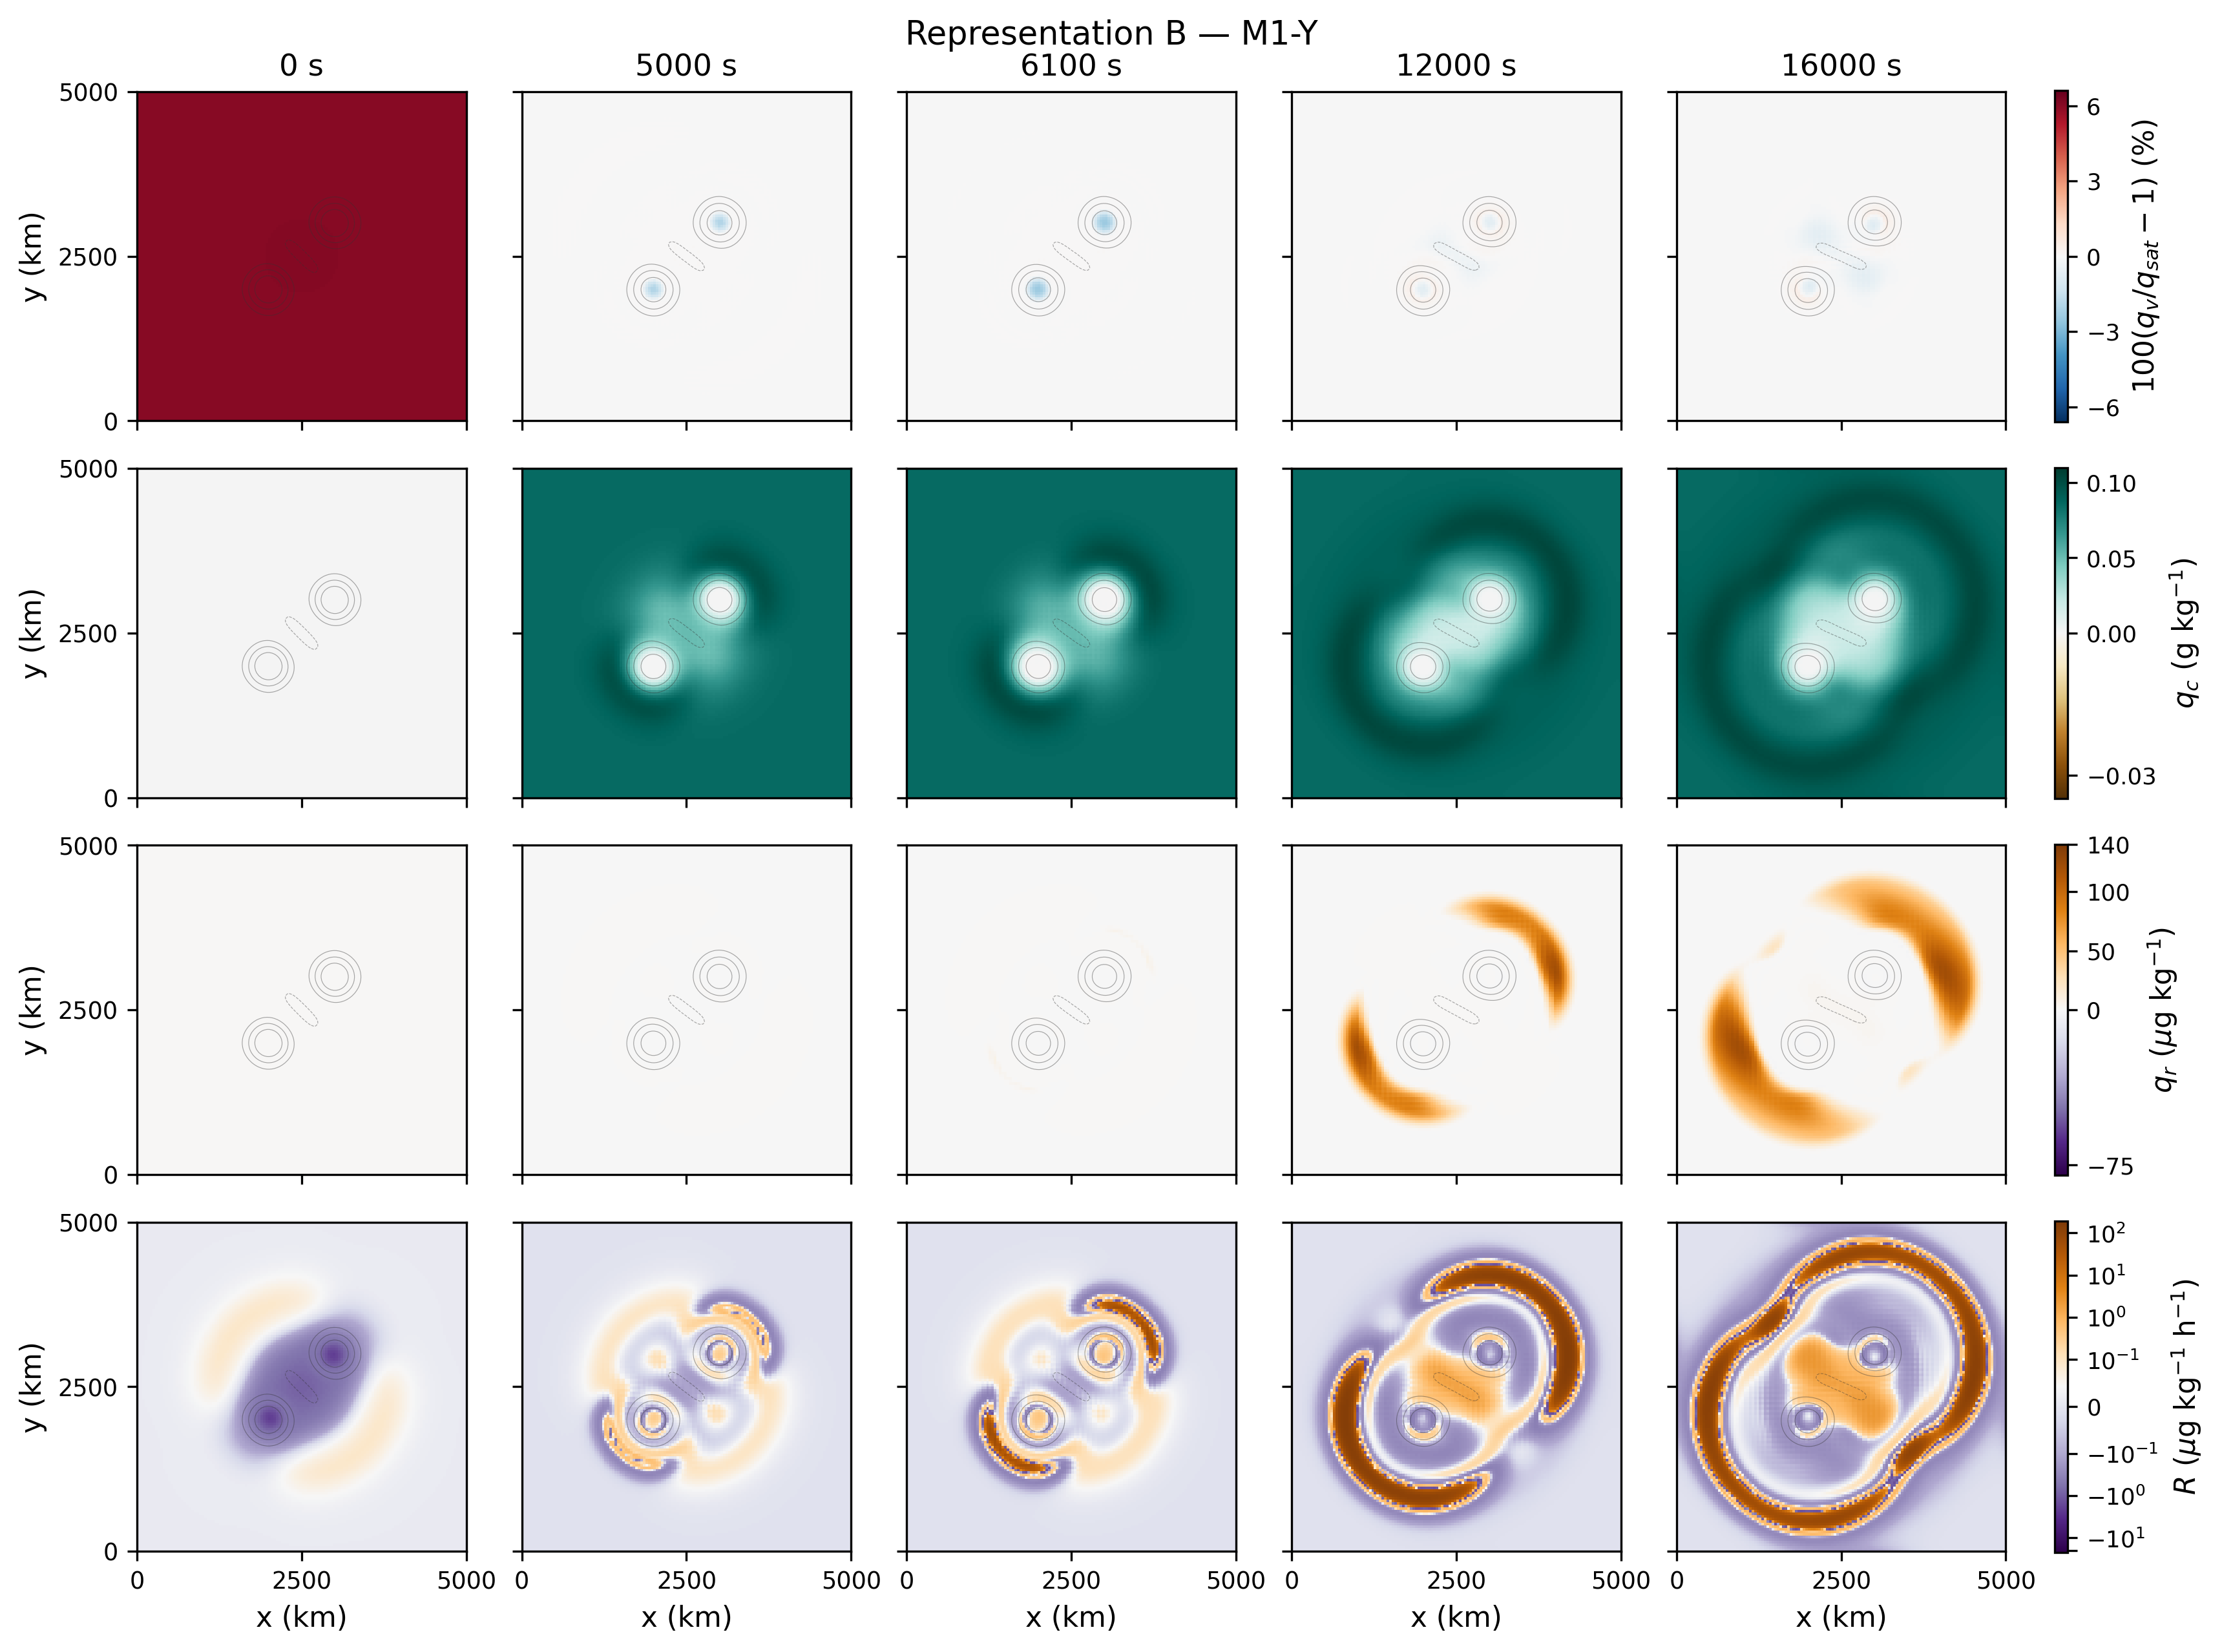
\includegraphics[width=\textwidth]{gallery_repB_M1Y.png}
	\caption{Same as figure \ref{fig:hybrid_truth_reference} but for Representation-B evolution using M1-Y.}
	\label{fig:hybrid_B_M1Y}
\end{figure}

\begin{figure}[p]
	\centering
	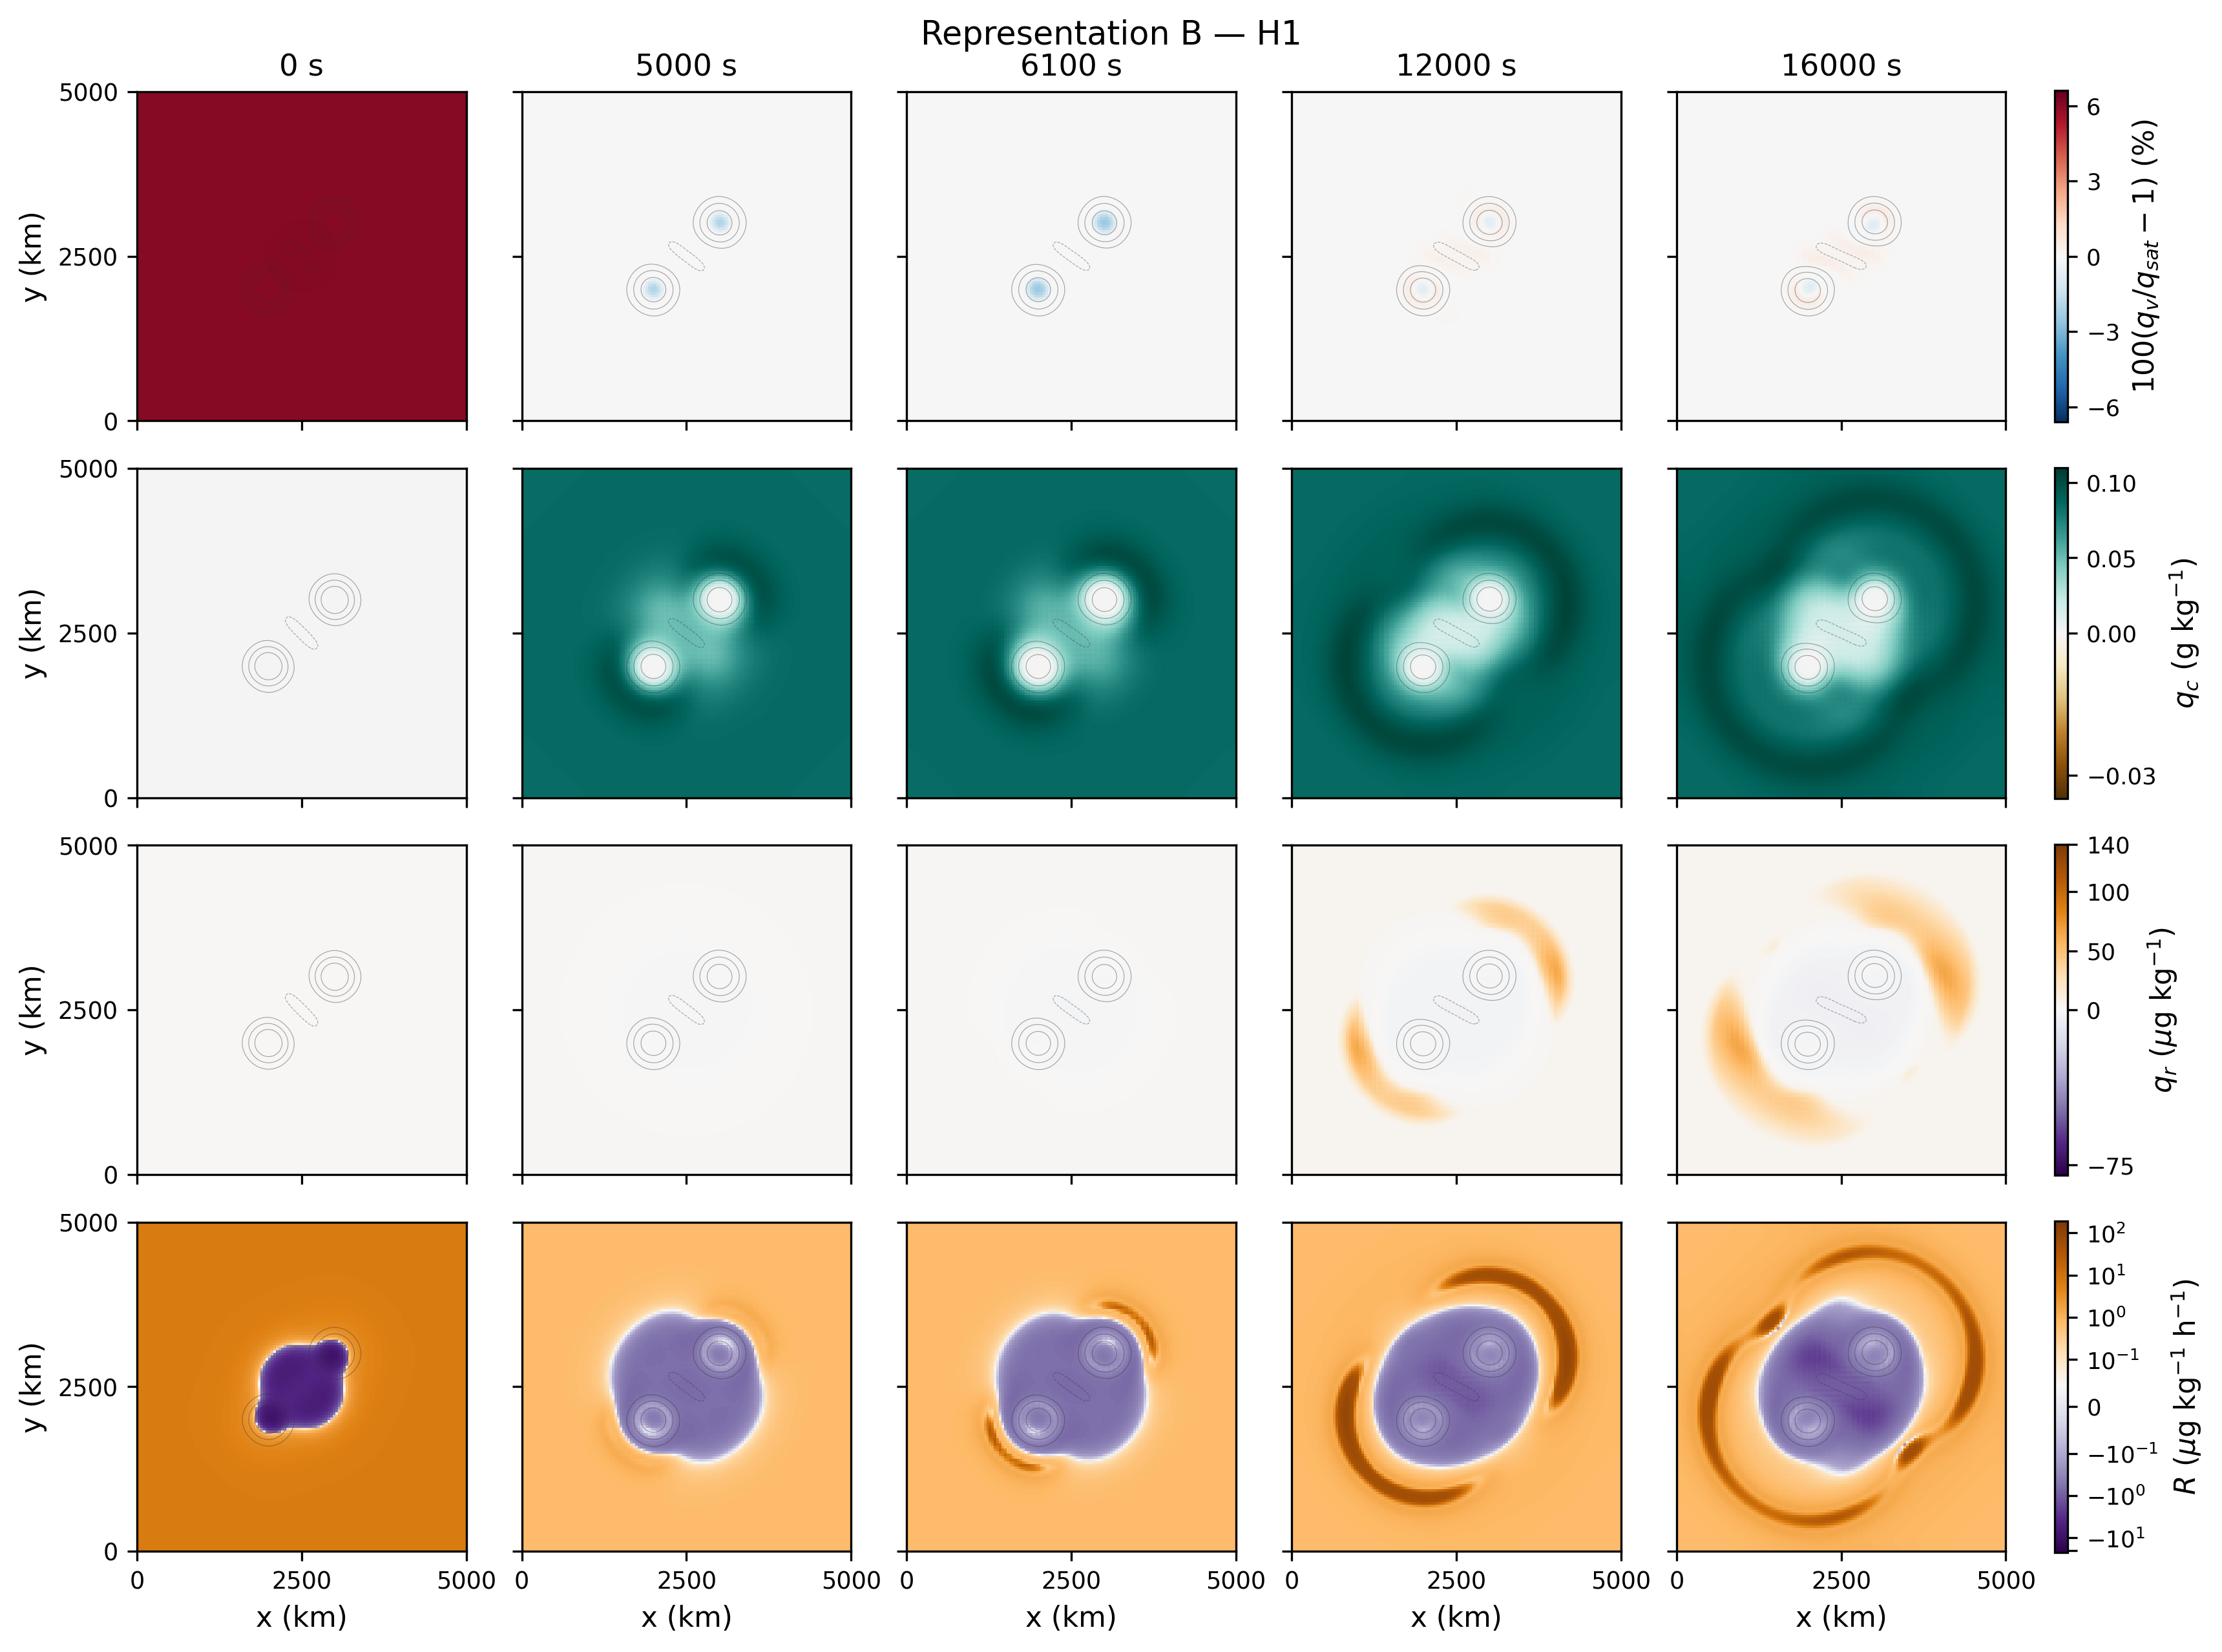
\includegraphics[width=\textwidth]{gallery_repB_H1.png}
	\caption{Same as figure \ref{fig:hybrid_truth_reference} but for Representation-B evolution using M2-Y/H1.}
	\label{fig:hybrid_B_H1}
\end{figure}

\begin{figure}[p]
	\centering
	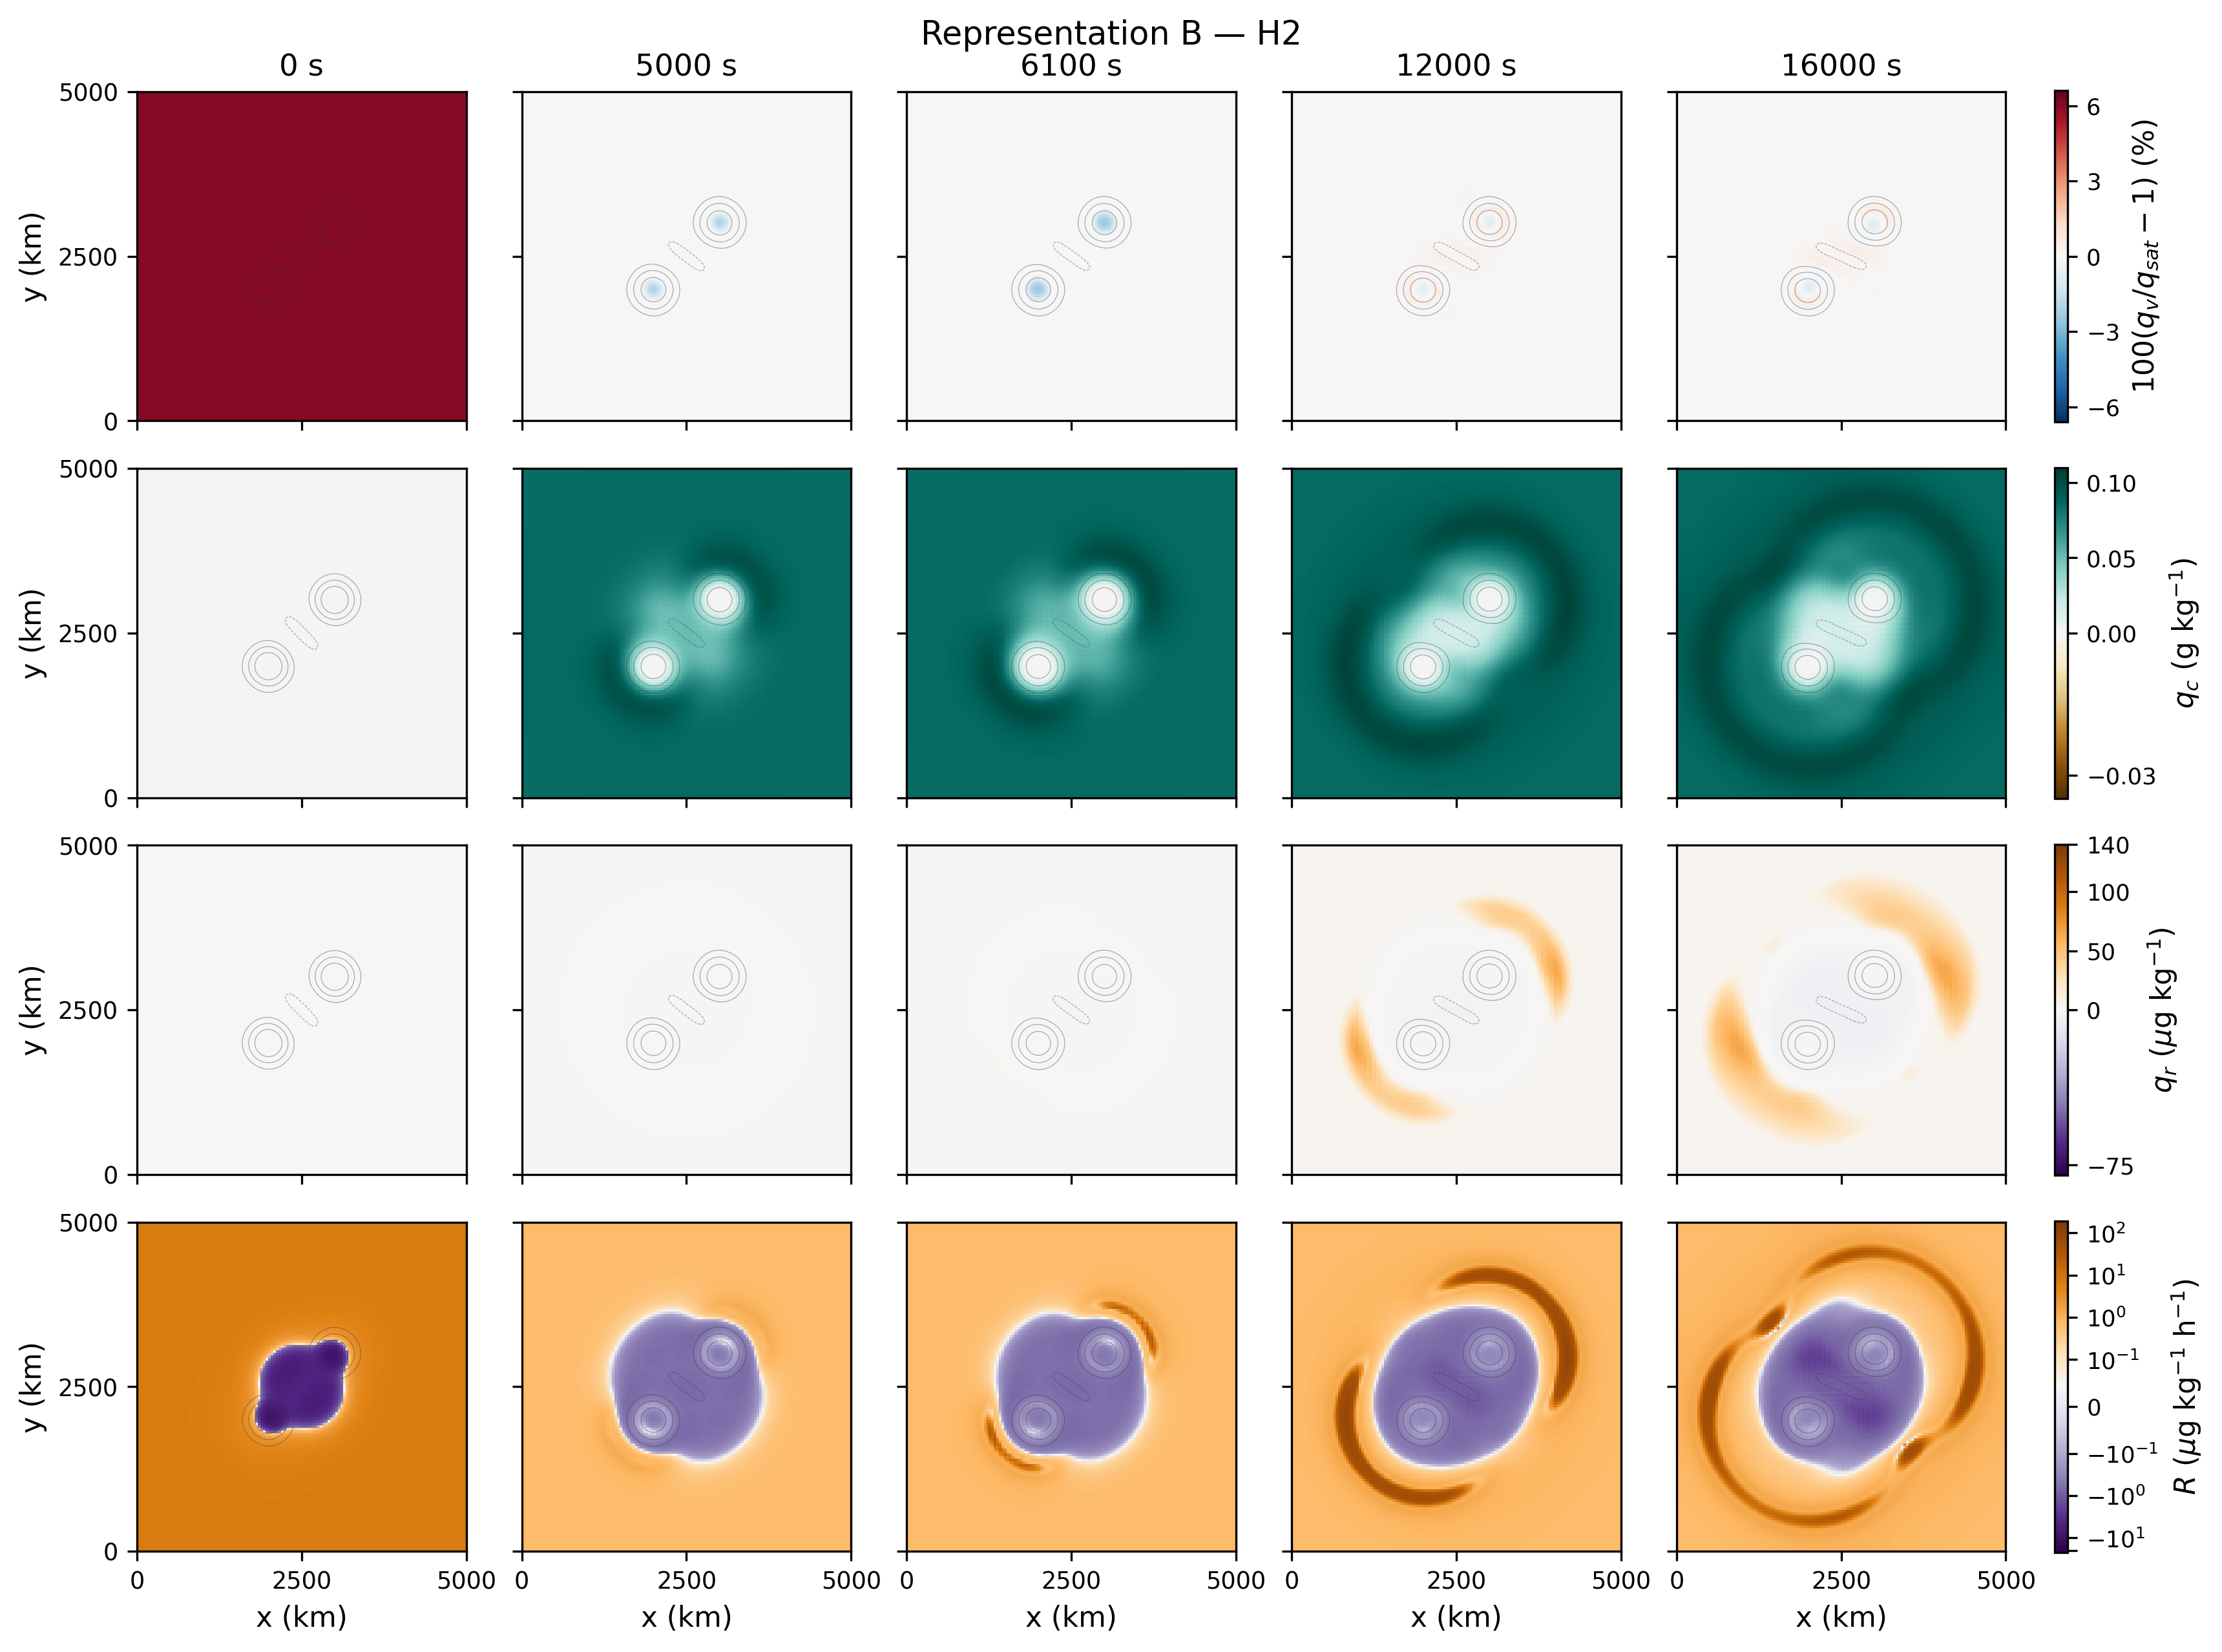
\includegraphics[width=\textwidth]{gallery_repB_H2.png}
	\caption{Same as figure \ref{fig:hybrid_truth_reference} but for Representation-B evolution using H2.}
	\label{fig:hybrid_B_H2}
\end{figure}

\begin{figure}[p]
	\centering
	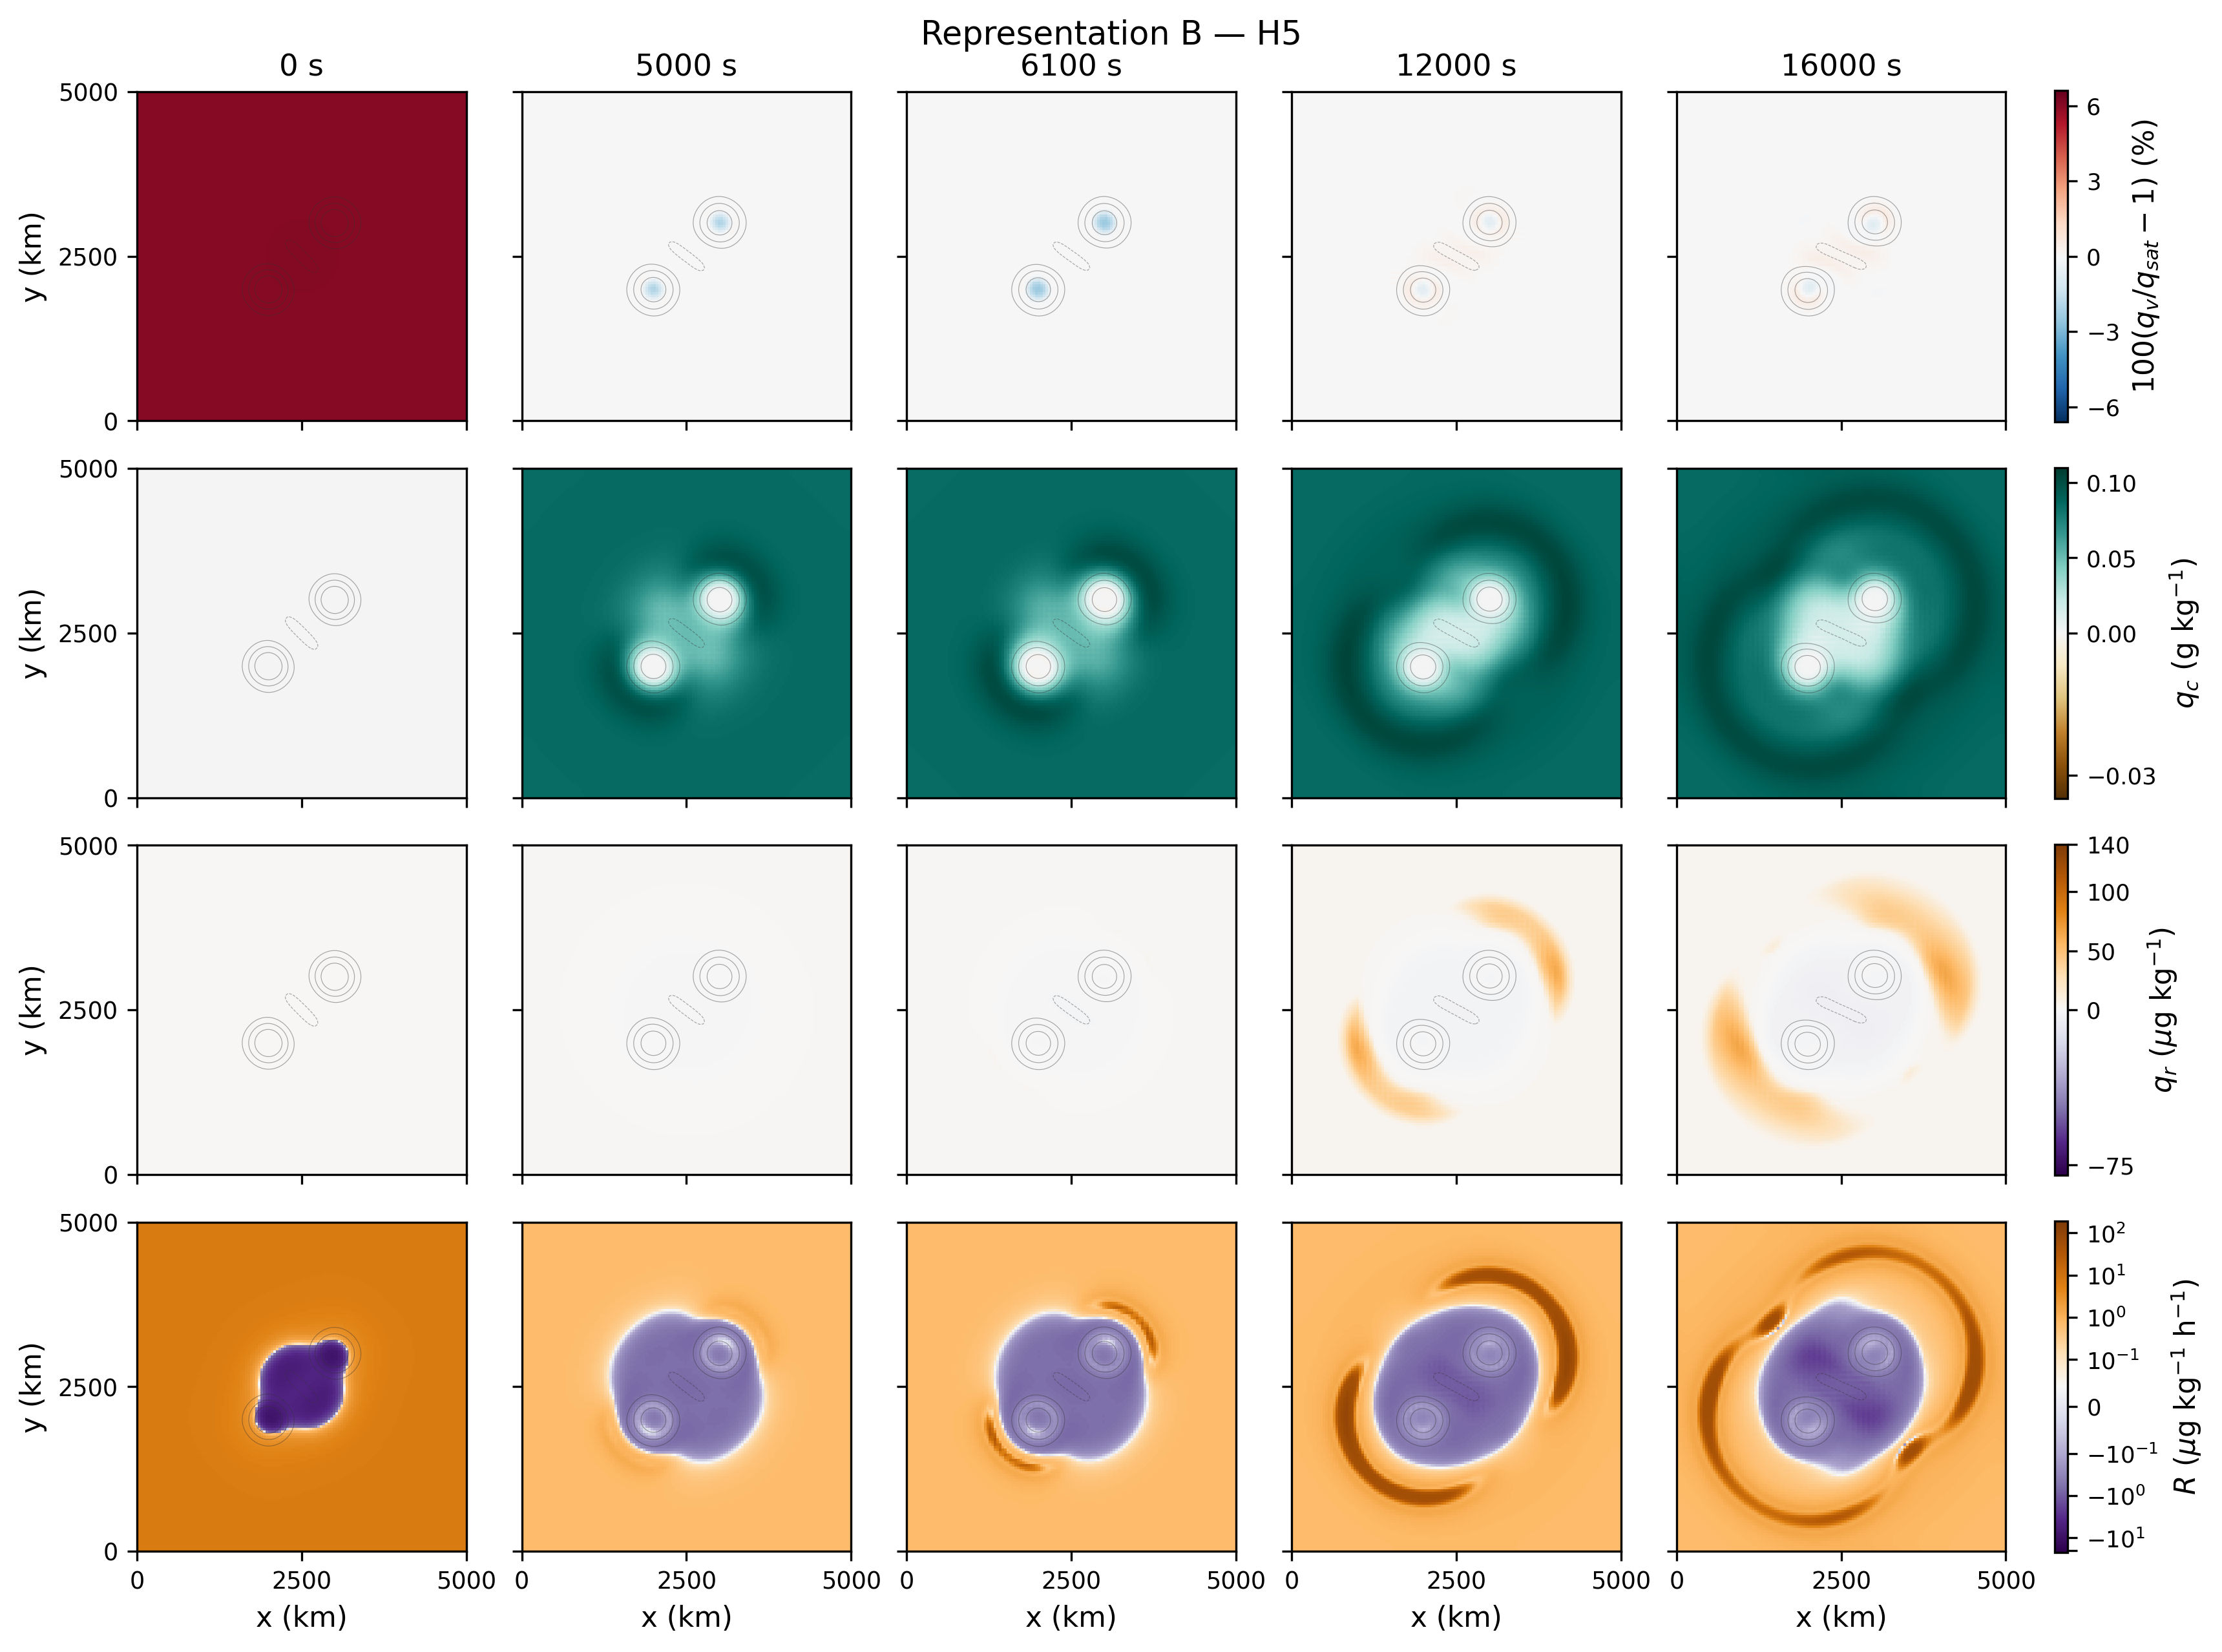
\includegraphics[width=\textwidth]{gallery_repB_H5.png}
	\caption{Same as figure \ref{fig:hybrid_truth_reference} but for Representation-B evolution using H5.}
	\label{fig:hybrid_B_H5}
\end{figure}

\clearpage


\subsection{Representation C}

Representation C produces a qualitatively different outcome. The M1-Y model (figure \ref{fig:hybrid_C_M1Y})
retains broadly truth-like cloud and positive rain-band morphology through the
simulation, although its effective rain-production field is spatially
oscillatory and contains both positive and negative structures. Thus a
reasonably accurate state evolution can coexist with substantial freedom in
the underlying unconstrained source representation.

The H1 (figure \ref{fig:hybrid_C_H1})), H2 (figure \ref{fig:hybrid_C_H2})), and H5 figure \ref{fig:hybrid_C_H5}) models, however, develop a distinctly unphysical water
partition. Negative rain water appears near the vortex cores by the
$5000~\mathrm{s}$ reference time and subsequently grows into broad
core-centered negative structures rather than the positive outer rain bands
seen in the truth solution. Negative cloud-water regions and stronger
subsaturation accompany this behavior. The same basic failure appears in H1
and H2 and becomes most pronounced for H5. This is consistent with
the conservation and water-partition diagnostics in
Sec.~\ref{sec:MLResults}: once the known two-rate source structure is removed,
the H1, H2, and H5 training sequence does not recover the missing physical
constraints.

Despite these large moisture errors, the relative-vorticity contours remain
visually close to the common two-vortex skeleton. The deterioration is
therefore concentrated primarily in the learned moist physics rather than in
a wholesale loss of the underlying flow structure. At least, keeping dynamical core non-ML has a value in this case.

\begin{figure}[p]
	\centering
	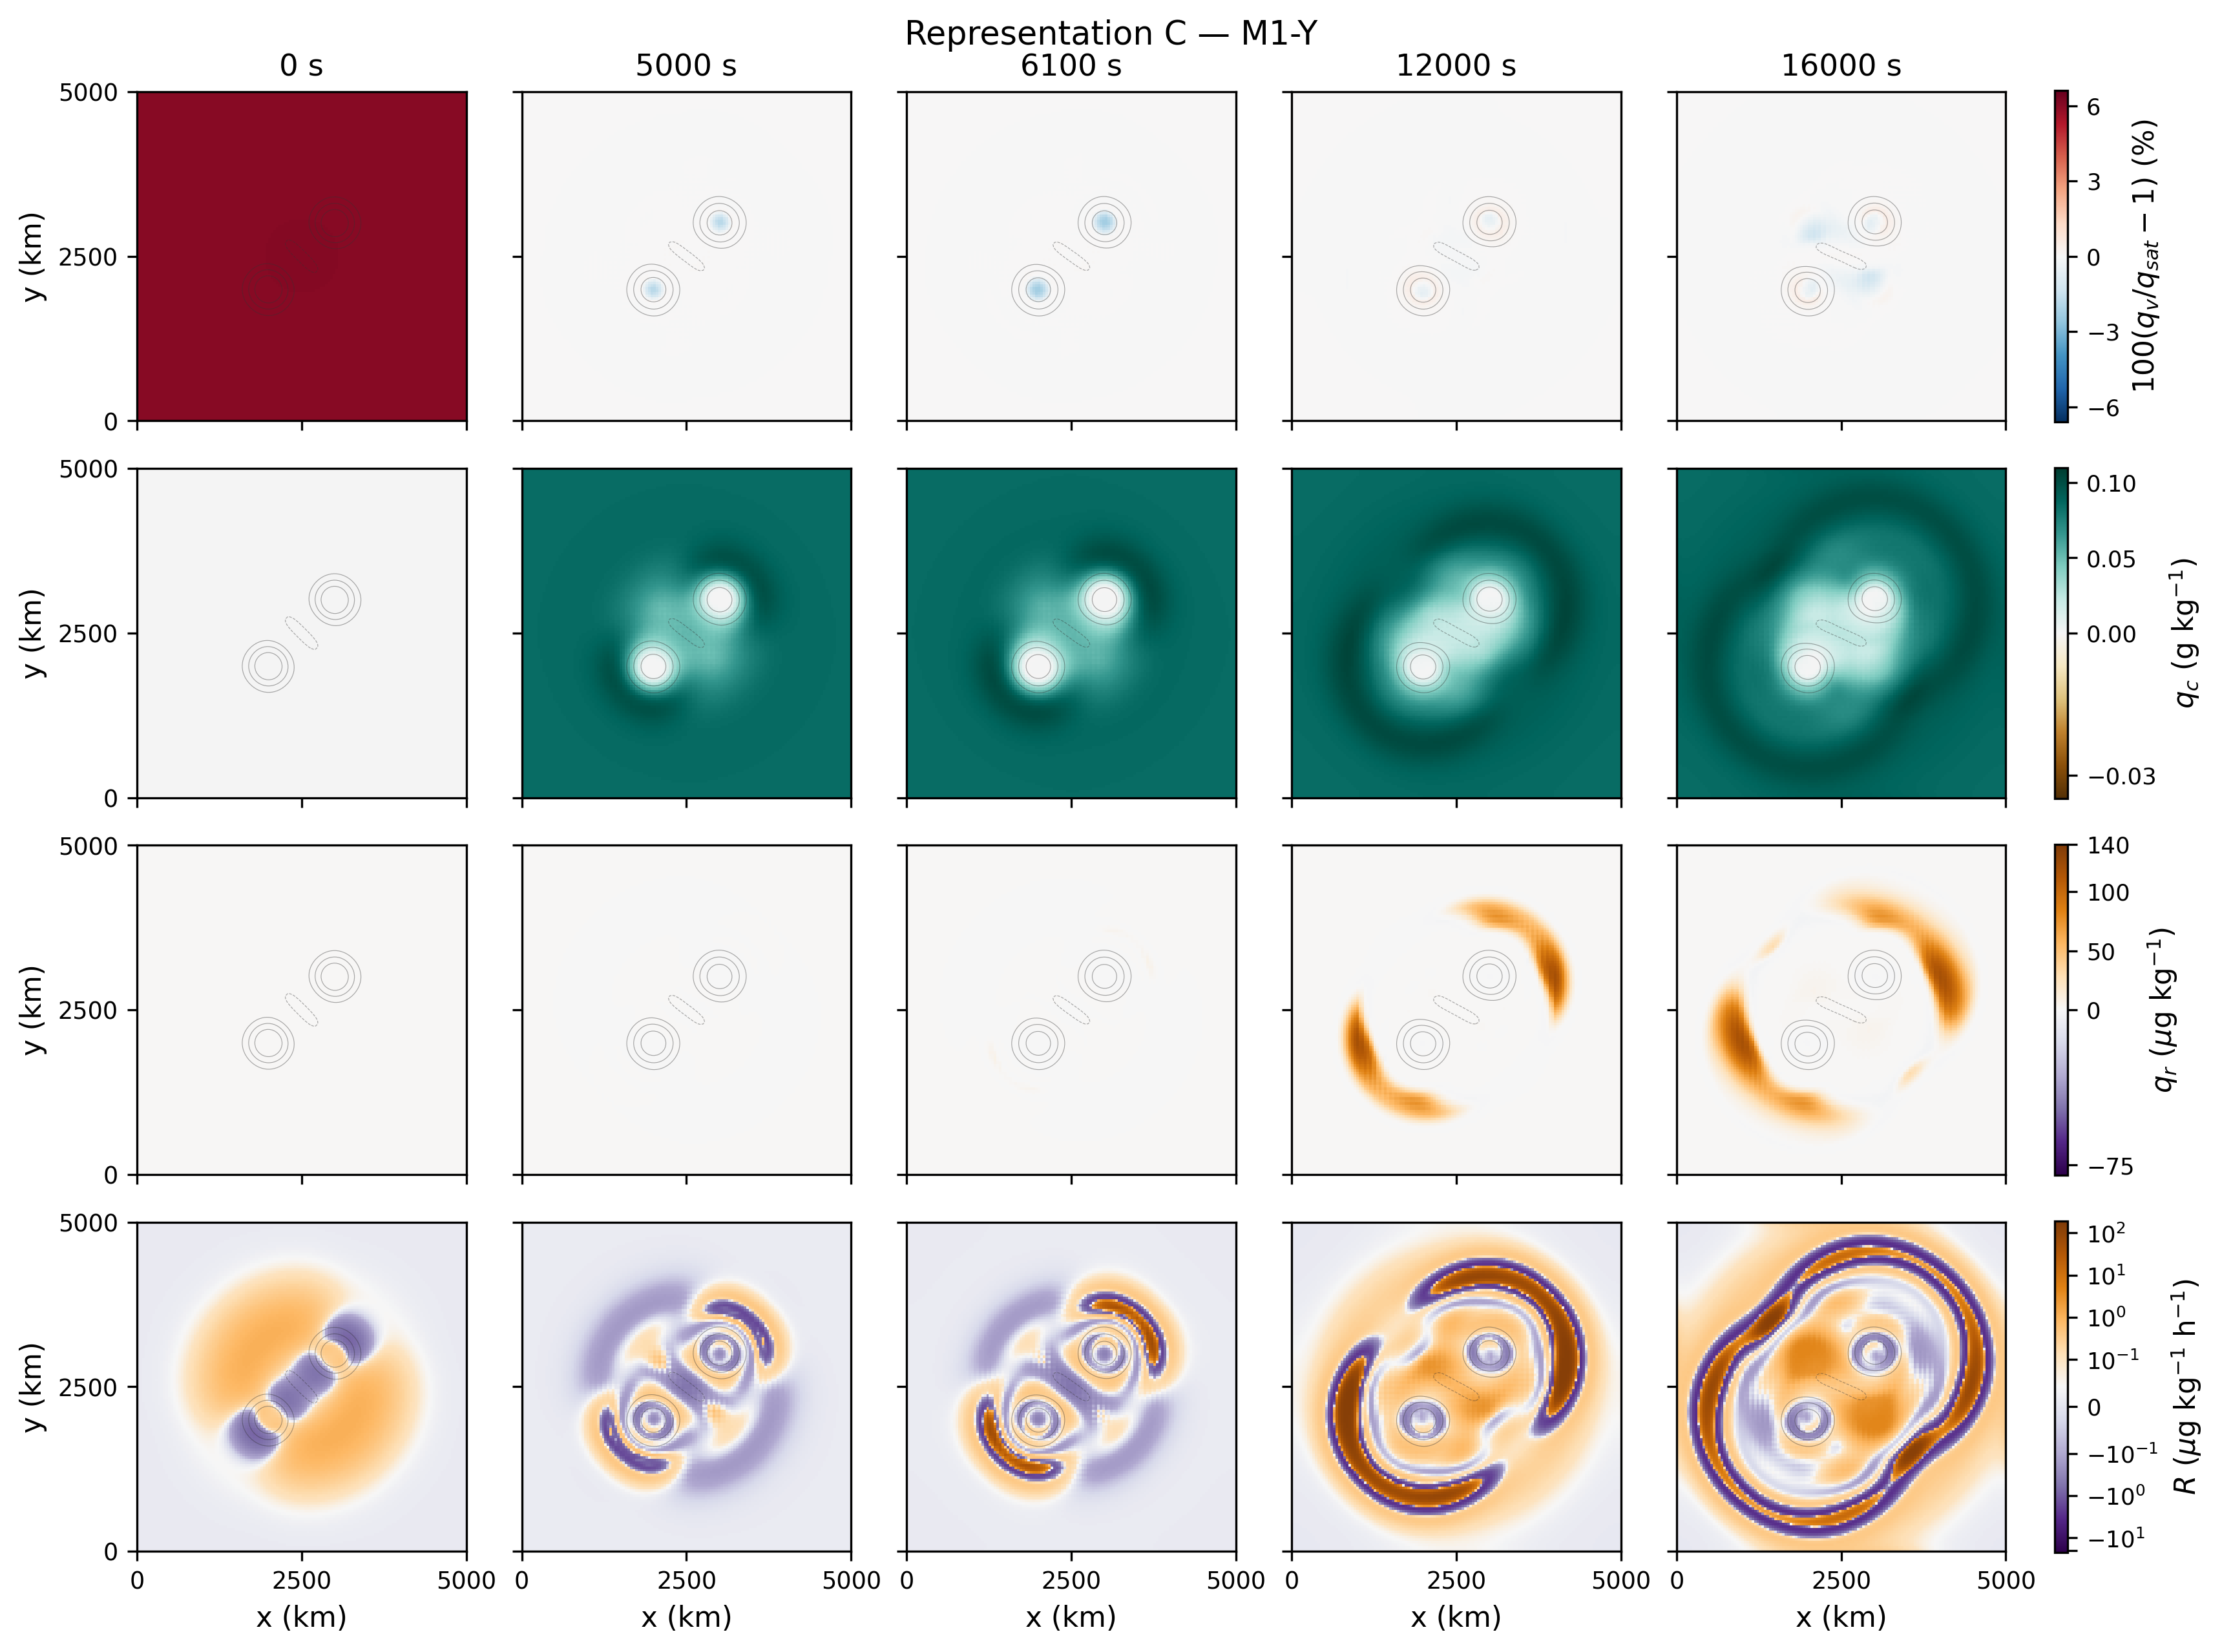
\includegraphics[width=\textwidth]{gallery_repC_M1Y.png}
	\caption{Same as figure \ref{fig:hybrid_truth_reference} but for Representation-C evolution using M1-Y.}
	\label{fig:hybrid_C_M1Y}
\end{figure}

\begin{figure}[p]
	\centering
	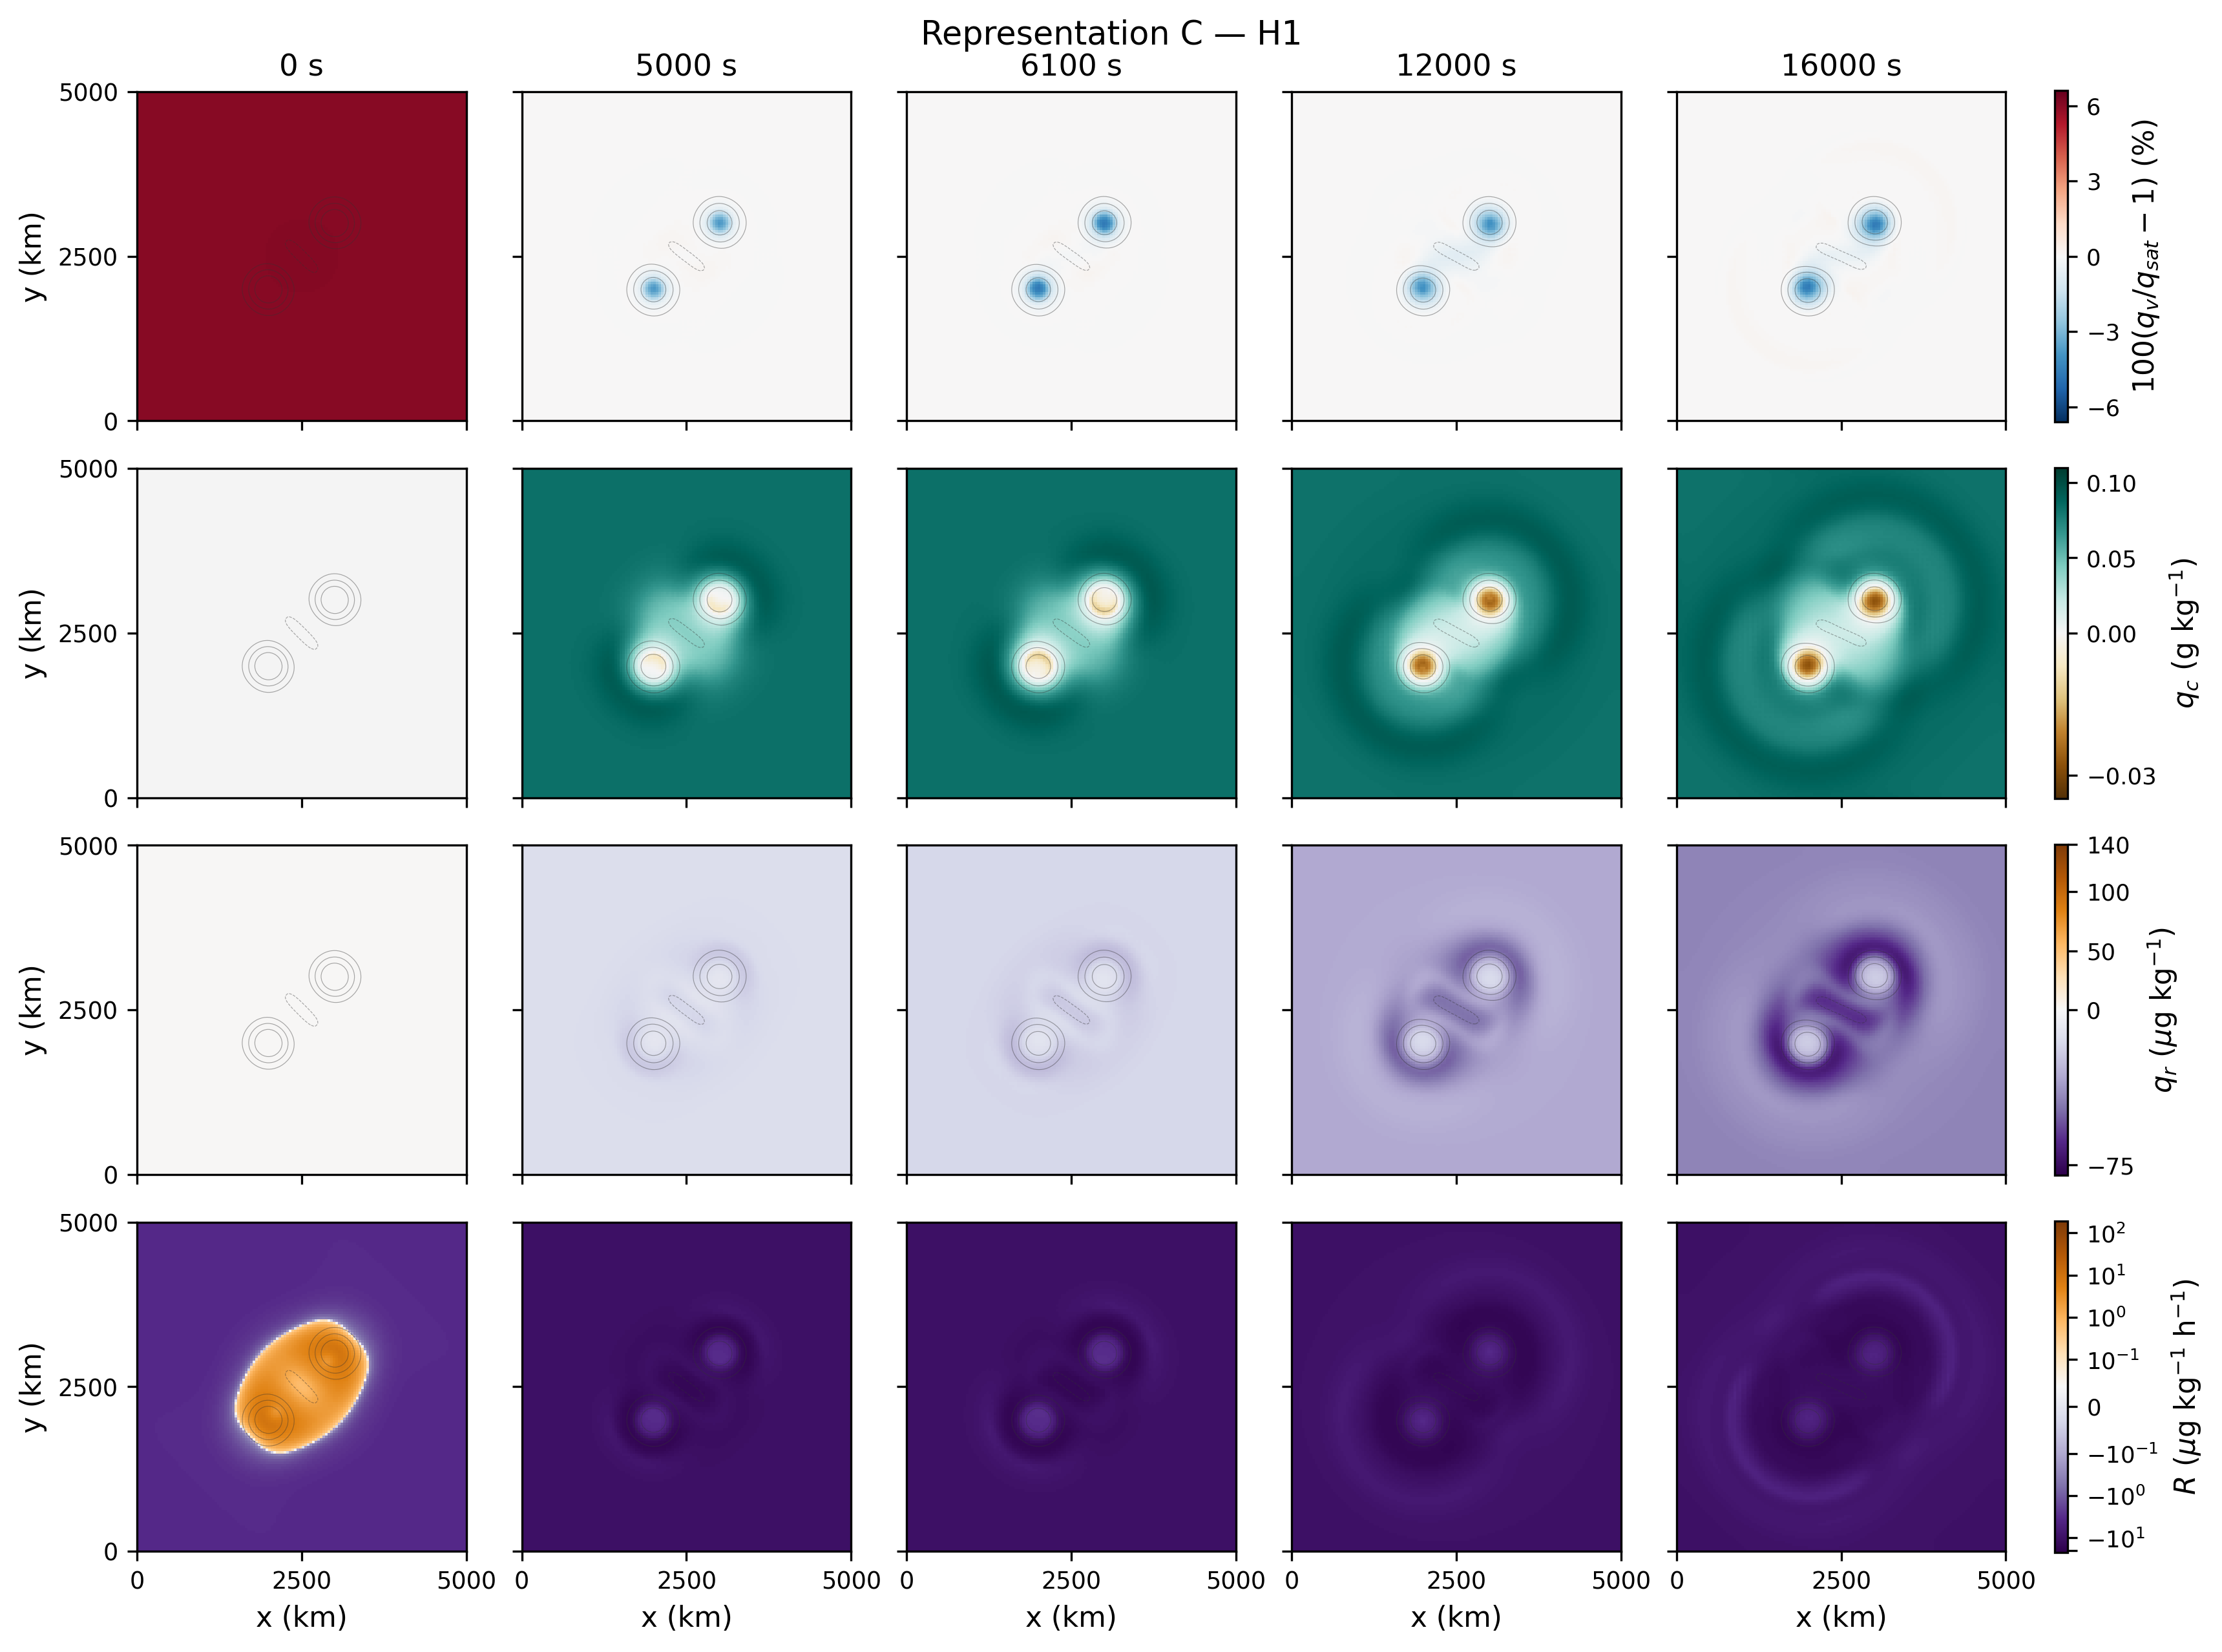
\includegraphics[width=\textwidth]{gallery_repC_H1.png}
	\caption{Same as figure \ref{fig:hybrid_truth_reference} but for Representation-C evolution using M2-Y/H1.}
	\label{fig:hybrid_C_H1}
\end{figure}

\begin{figure}[p]
	\centering
	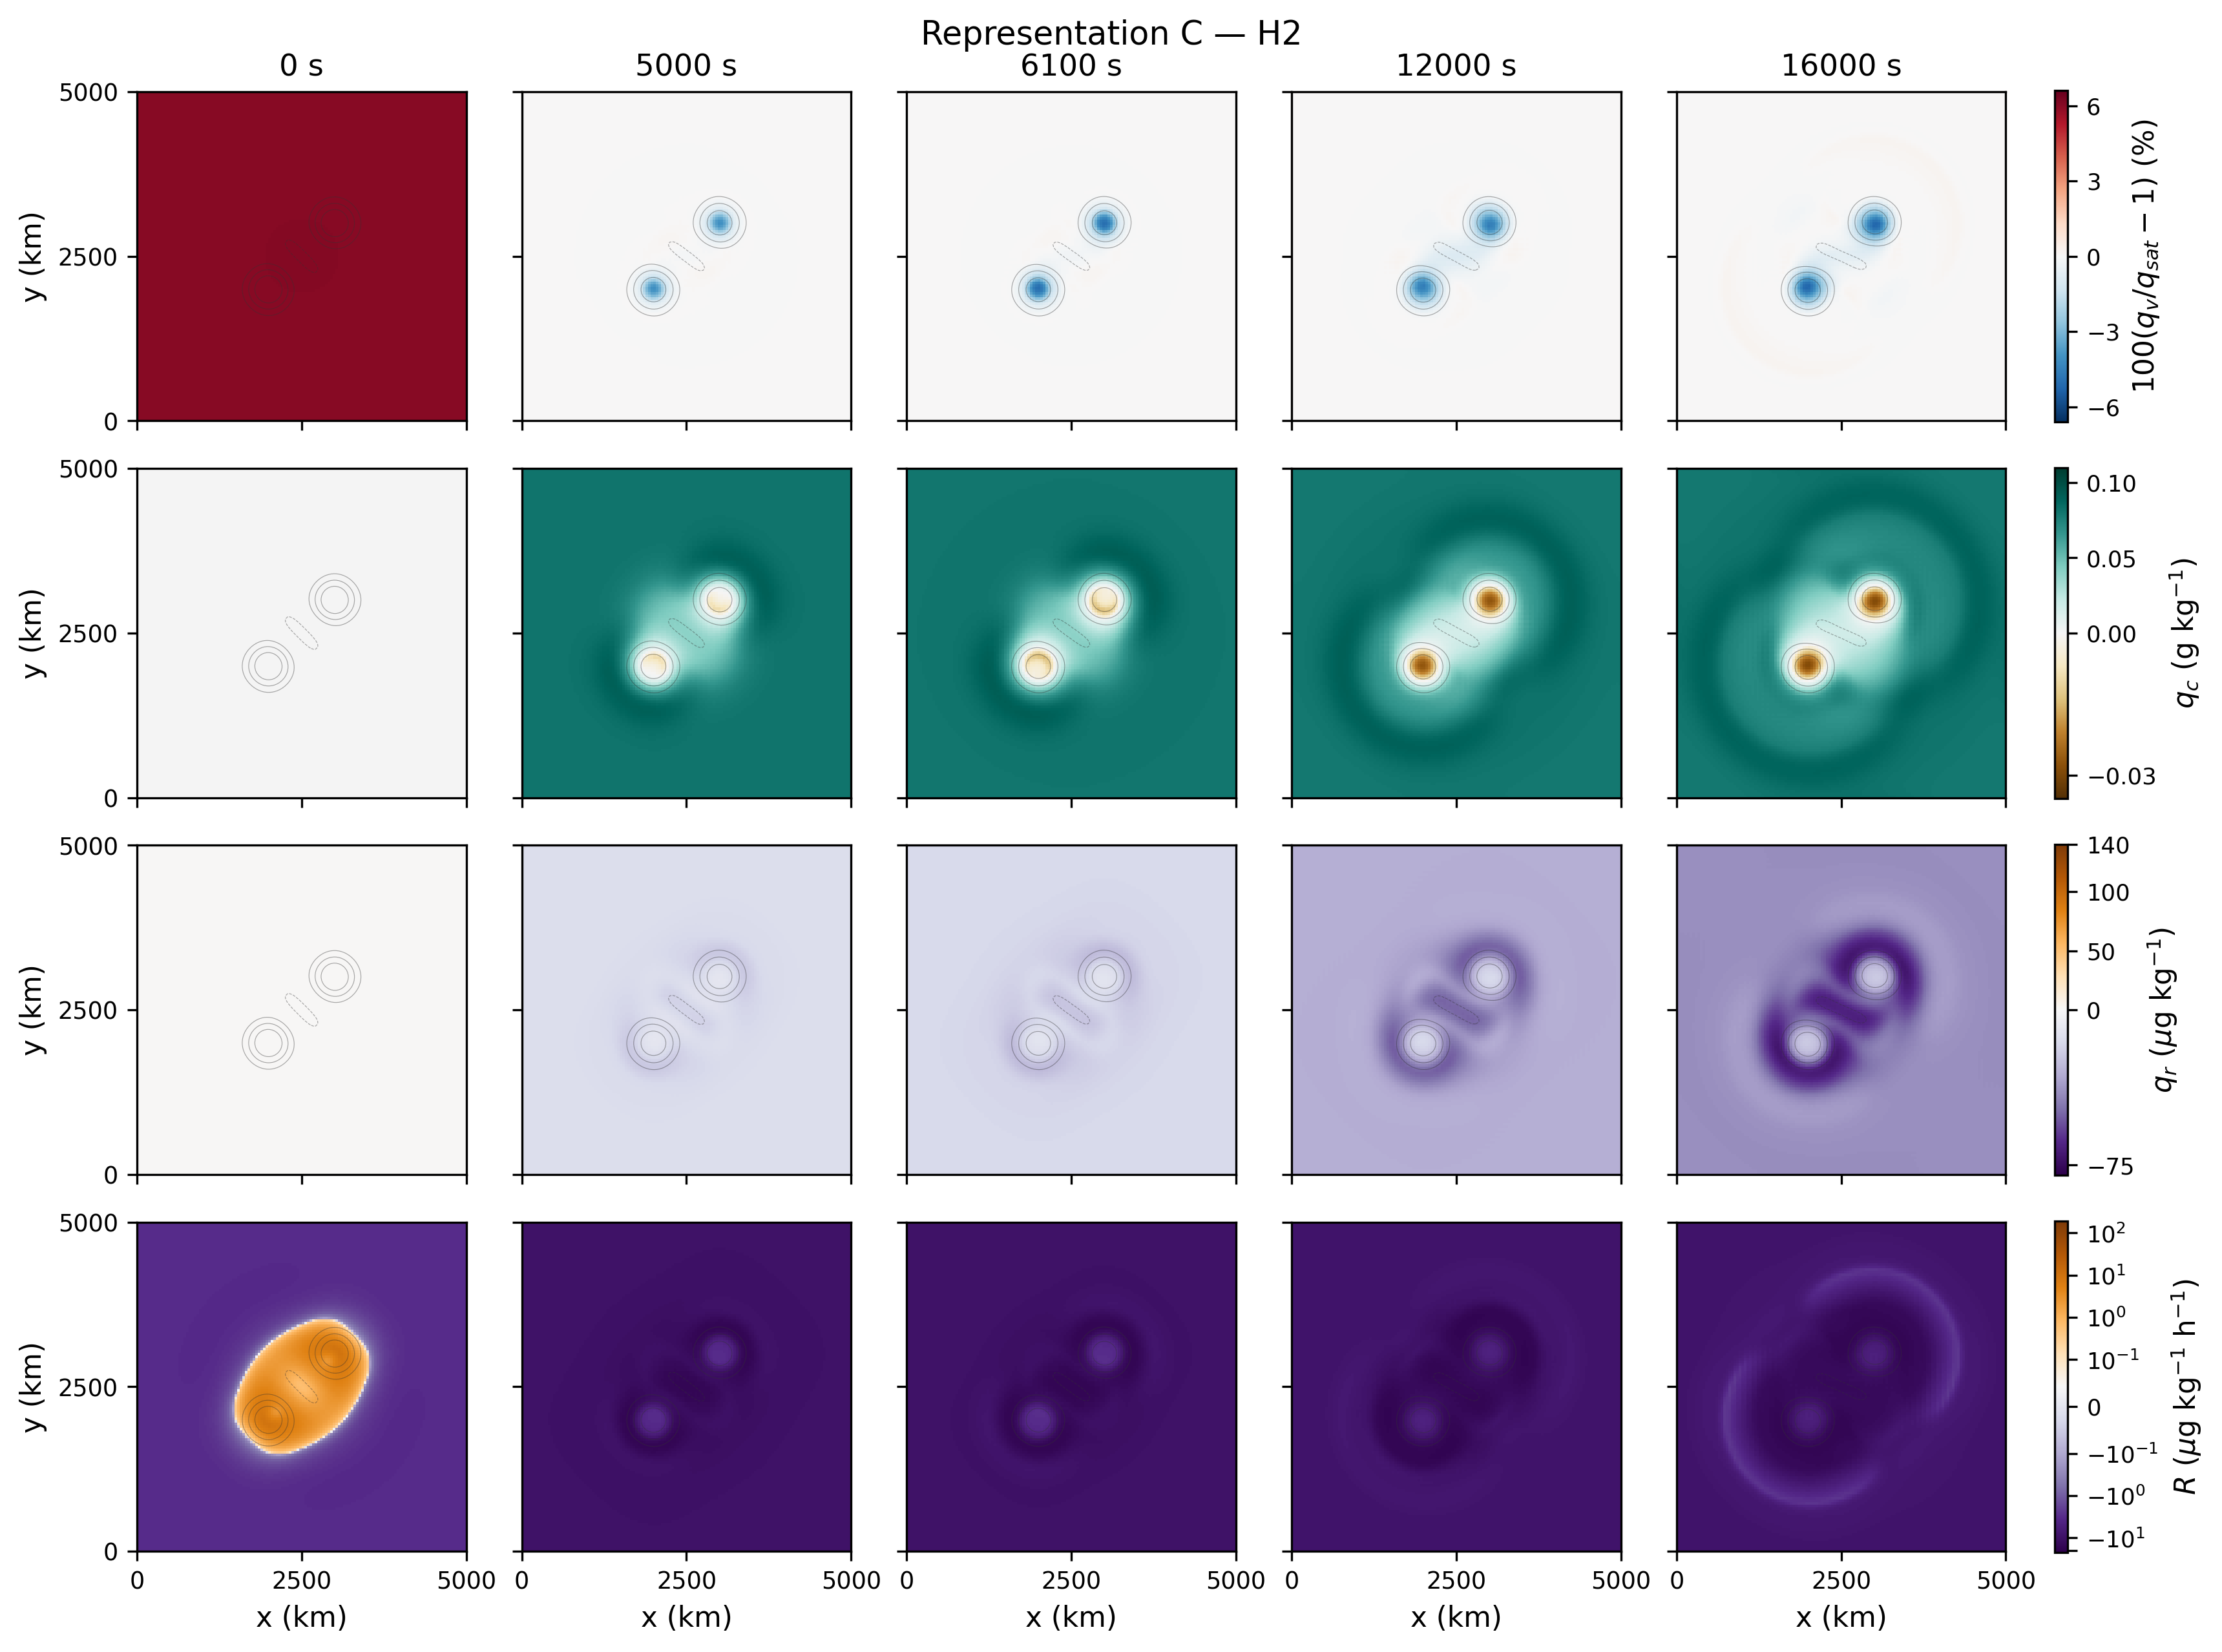
\includegraphics[width=\textwidth]{gallery_repC_H2.png}
	\caption{Same as figure \ref{fig:hybrid_truth_reference} but for Representation-C evolution using H2.}
	\label{fig:hybrid_C_H2}
\end{figure}

\begin{figure}[p]
	\centering
	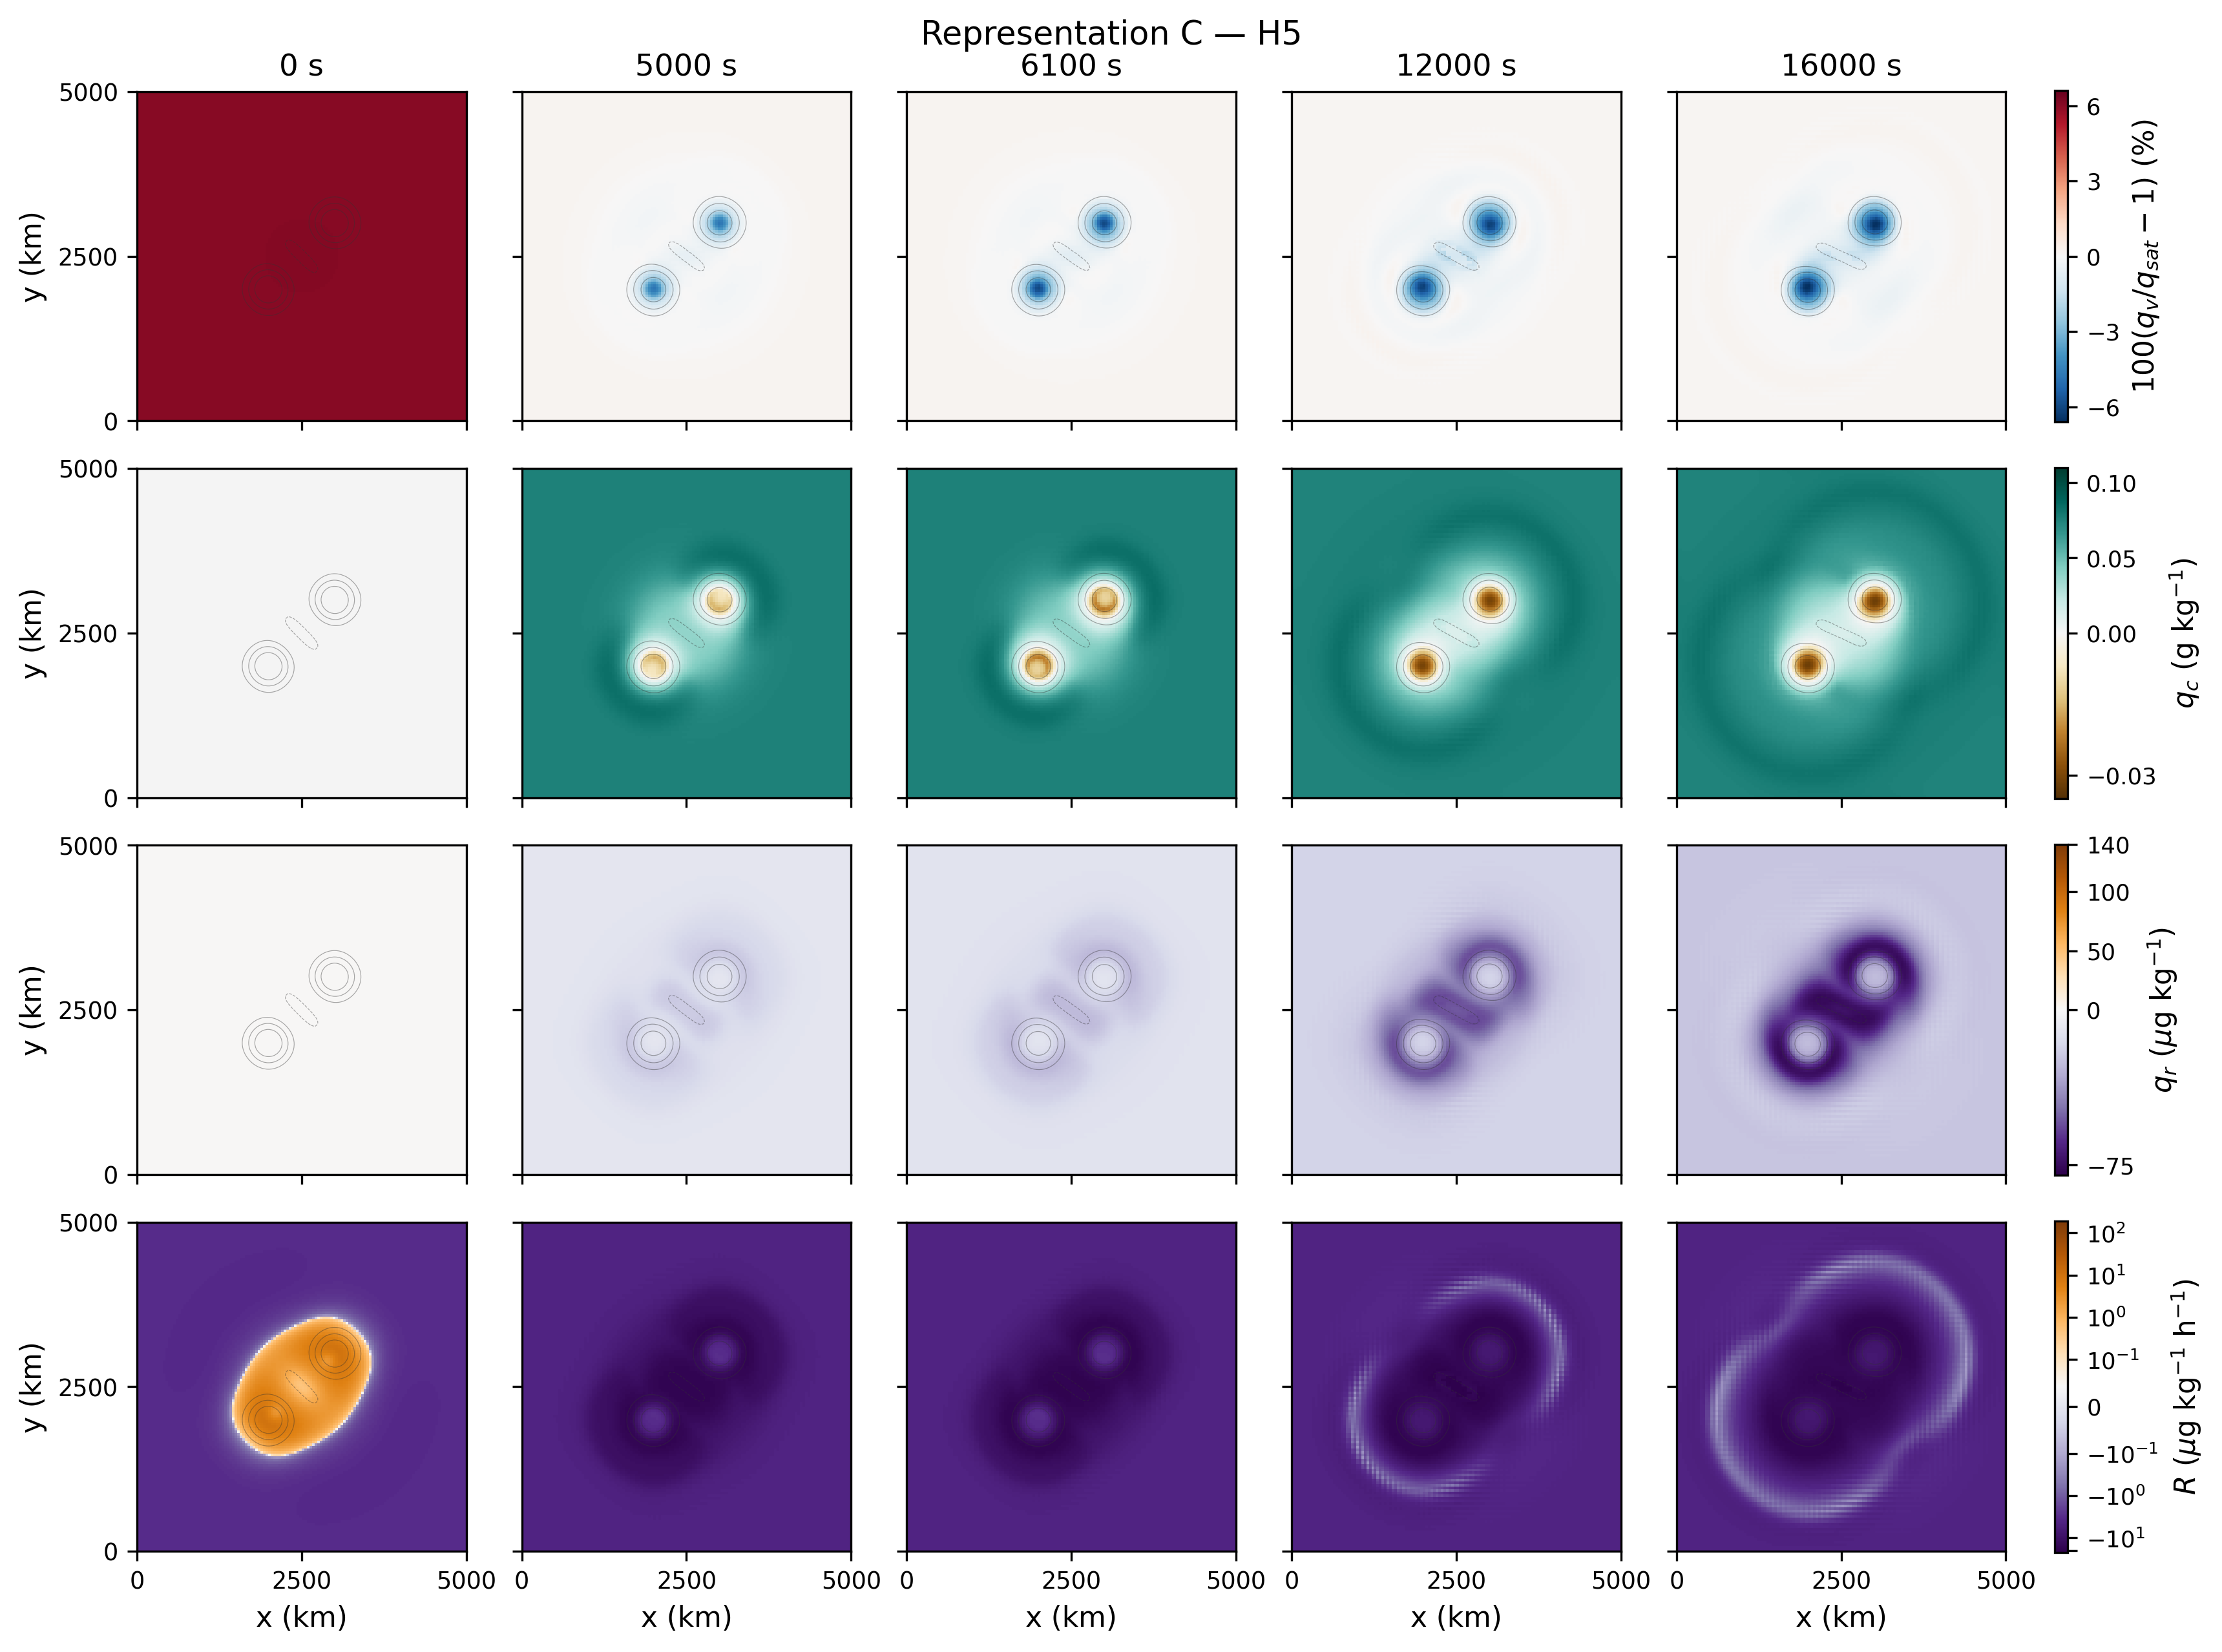
\includegraphics[width=\textwidth]{gallery_repC_H5.png}
	\caption{Same as figure \ref{fig:hybrid_truth_reference} but for Representation-C evolution using H5.}
	\label{fig:hybrid_C_H5}
\end{figure}

\clearpage

The corresponding movies contain all 161 stored states and use the same fixed
color limits as the galleries. They provide the continuous-time view of these
dynamics and confirm the qualitative behavior identified above: Representation
A remains spatially robust across the four training objectives, Representation
B preserves the state morphology despite substantial differences in the
learned rain-production field, and Representation C develops increasingly
unphysical moisture partitioning for H1, H2, and H5.
	
	
	\section{Conclusions}\label{sec:Conclusions}

	We study several ways of learning a known moist-physics
	parameterization within the discretized thermal shallow-water equations (DIMSWE). The
	study separated three choices: the physical structure imposed
	on the learned parameterization, the quantity used in the training loss (and hence the necessity of online training), and
	the extent to which model-generated states are included during training.
	
	A first result is that direct regression of the local moist physics at the
	state where the parameterization is actually evaluated provides a strong
	baseline. In M1-Y, the network is trained directly on the pre-moist state
	$Y^\star=P(X^\star)$. This approach is entirely offline and does not require
	differentiating through the timestep or recursively evolving the learned
	model. Nevertheless, the resulting models remain stable over the full
	DoubleVortex simulation and, particularly for the structured
	Representations A and B are designed for conservation and reproduce the global evolution accurately.
	
	The one-step H1/M2-Y objective and the recursive H2 and H5 objectives do not
	provide a uniform improvement over direct regression of M1-Y. For
	Representations A and B, the state-based models (all except M1-Y) can reduce the later-time
	error in the phase-change rate $A$, but this does not imply more accurate
	recovery of every learned physical process. In Representation B, for example,
	M1-Y reproduces the analytical rain-production law much more accurately than
	H1, H2, or H5, even though all four models produce comparatively accurate
	deployed state trajectories. Thus a learned model can reproduce the resolved
	state well while representing an individual physical process substantially
	less faithfully.
	
	The strongest distinction arises from the choice of learned-physics
	representation. Representation A learns only the phase-change rate and retains
	both the analytical rain law and the prescribed moist-source structure.
	Its deployed evolution is robust across all four training objectives.
	Representation B additionally learns the rain-production rate but retains the
	known algebraic coupling among the moist tendencies. Its deployed states also
	remain accurate and total-water conservation is preserved, although the
	learned rain law is considerably more sensitive to the training objective.
	Representation C instead learns the four moist-source components independently.
	The resulting source is not constrained to satisfy the known total-water and
	thermodynamic identities or the physical two-rate source structure. Although
	M1-Y produces a comparatively accurate Representation-C model, the H1, H2,
	and H5 sequence develops progressively larger conservation errors, unphysical
	cloud--rain partitioning, and negative discrete moisture values.
	
	The recursive calculations provide an additional caution. The H2 and H5
	training errors decrease over their respective optimization stages, but for
	Representation C the error after the full 160-step deployed calculation
	increases. Improving a two- or five-step training objective therefore does not
	necessarily improve the much longer deployed trajectory. In the present
	study, the recursive stages were limited to only 20 optimization iterations
	and were initialized sequentially from the preceding model, so these results
	should not be interpreted as a definitive comparison of rollout horizon alone.
	
	All learning strategies also show a substantial difference between errors over
	the training portion of the DoubleVortex trajectory and the later evaluation
	portion. The latter is a continuation of the same deterministic flow rather
	than a new physical regime or initial condition, so the observed degradation
	already indicates that accurate fitting over a large number of spatial samples
	does not guarantee temporal generalization as the model state evolves.
	
	Taken together, the results suggest that increasing the complexity of the
	training objective is not by itself sufficient to improve a learned physical
	parameterization. For this problem, two simpler considerations are at least as
	important: training the network on the state at which the parameterization is
	actually called, and retaining known physical structure in the learned source.
	Once these are satisfied, direct offline regression can already provide stable
	and accurate long-time deployment, while one-step and recursive state-based
	training provide more limited and representation-dependent benefits.
	
	Several extensions remain important. The present calculations use a single
	DoubleVortex trajectory, a fixed neural-network architecture, and a single
	initialization. Broader training data, additional flow realizations, larger
	networks, and longer optimization of the recursive objectives would help
	separate limitations due to data coverage, model capacity, and optimization.
	The current networks also do not enforce positivity, and Representations B and
	C do not impose the analytical sign or threshold structure of the learned rain
	process. Incorporating such physical constraints, as well as using specific
	variables such as $(h,b,q_v,q_c,B)$ that more directly expose the analytical
	moist-physics dependencies, provides a natural direction for future work.


	\bibliographystyle{plain}
	\bibliography{DIMSWEML}
\end{document}